\documentclass[11pt]{article}%
\usepackage{graphicx}
\usepackage{amsmath}
\usepackage{mathtools} % \vdotswithin
\usepackage{amsfonts}
\usepackage{amssymb}
\usepackage{epstopdf}
\usepackage{booktabs}
\graphicspath{ {./P3FiguresPDF/} }
\setcounter{MaxMatrixCols}{30}
\newtheorem{theorem}{Theorem}
\newtheorem{acknowledgement}[theorem]{Acknowledgement}
\newtheorem{algorithm}[theorem]{Algorithm}
\newtheorem{axiom}[theorem]{Axiom}
\newtheorem{case}[theorem]{Case}
\newtheorem{claim}[theorem]{Claim}
\newtheorem{conclusion}[theorem]{Conclusion}
\newtheorem{condition}[theorem]{Condition}
\newtheorem{conjecture}[theorem]{Conjecture}
\newtheorem{corollary}[theorem]{Corollary}
\newtheorem{criterion}[theorem]{Criterion}
\newtheorem{definition}[theorem]{Definition}
\newtheorem{example}[theorem]{Example}
\newtheorem{exercise}[theorem]{Exercise}
\newtheorem{lemma}[theorem]{Lemma}
\newtheorem{notation}[theorem]{Notation}
\newtheorem{problem}[theorem]{Problem}
\newtheorem{proposition}[theorem]{Proposition}
\newtheorem{remark}[theorem]{Remark}
\newtheorem{solution}[theorem]{Solution}
\newtheorem{summary}[theorem]{Summary}
\newenvironment{proof}[1][Proof]{\textbf{#1.} }{\ \rule{0.5em}{0.5em}}
\setlength{\textwidth}{6.25in} \setlength{\textheight}{8.5in}
\setlength{\oddsidemargin}{-1mm} \setlength{\evensidemargin}{-1mm}
\setlength{\topmargin}{-0.25in}
\parskip 1.5ex
\long
\def\symbolfootnote[#1]#2
{\begingroup
\def\thefootnote{\fnsymbol{footnote}}
\footnote[#1]{#2}\endgroup}
\title{\textbf{\huge\raggedleft Project 4}}
\author{Nicholas Sebasco}
\date{\today}

\begin{document}

%\maketitle
\begin{titlepage}
    \begin{center}
        \vspace*{1cm}
            
        \Huge
        \textbf{Methods of Polynomial Interpolation}
            
        \vspace{0.5cm}
        \LARGE
        An Analysis of Error and Computational Performance
            
        \vspace{1.5cm}
            
        \textbf{Nicholas Sebasco}
            
        \vfill
            
       	Advisor: Dr. Lei Hsin Kuo\\
        %Doctor of Philosophy
            
        \vspace{0.8cm}
            
        
\includegraphics[width=0.4\textwidth]{logo}
            
        \Large
        Mathematics\\
        University of West Florida\\
        United States\\
        August 8th 2021
            
    \end{center}
\end{titlepage}


\section*{Introduction}
%
This research will compare and contrast methods of polynomial interpolation. The following functions will be approximated by degree $n$ polynomials, and their absolute errors and computational speed will be analyzed.

\begin{equation}
f\left(x\right) = Sin(x), x \in [0, 2\pi]
\end{equation}

\begin{equation}
g\left(x\right) = Sin(5x), x \in [0, 2\pi]
\end{equation}

\begin{equation}
h\left(x\right) = \dfrac{1}{1+x^2}, x \in [-5, 5]
\end{equation}

Each polynomial will be constructed for $ n = $ 5, 10, 15, 25, and 35 points. After construction, the polynomials will be plotted on $ n_t = 1000 $ test points. 6 curves for each $n$ value were created for two sets of figures. The first set of figures are plots of the 6 approximations along with the actual function. The second set of figures are plots of the error of each of the 6 curves. The figures regarding the error distributions are defined as: $\varepsilon:=\{|f(x_j) - p(x_j)|\}^m_{j=1}$, where $x_i = a + [b - a]\dfrac{i}{n_t}, i = 0, 1, ..., n_t$. The 6 curves are defined as:
\begin{enumerate}
\item Direct-Equal: The Direct method constructed on $n$ equally spaced points.
\item Direct-Chebyshev: The Direct method constructed on $n$ Chebyshev nodes.
\item Lagrange-Equal: A Lagrange polynomial constructed on $n$ equally spaced points.
\item Lagrange-Chebyshev: A Lagrange polynomial constructed on $n$ Chebyshev nodes.
\item Hermite-Equal: A Hermite polynomial constructed on $n$ equally spaced points.
\item Hermite-Chebyshev: A Hermite polynomial constructed on $n$ Chebyshev nodes.
\end{enumerate}

\newpage
% PAGE 2
\section*{Background}

% opening caption
\vspace{25pt}
\begin{figure}[htp]

\centering
\vspace{-20pt} % I can control the vertical spacing this way.
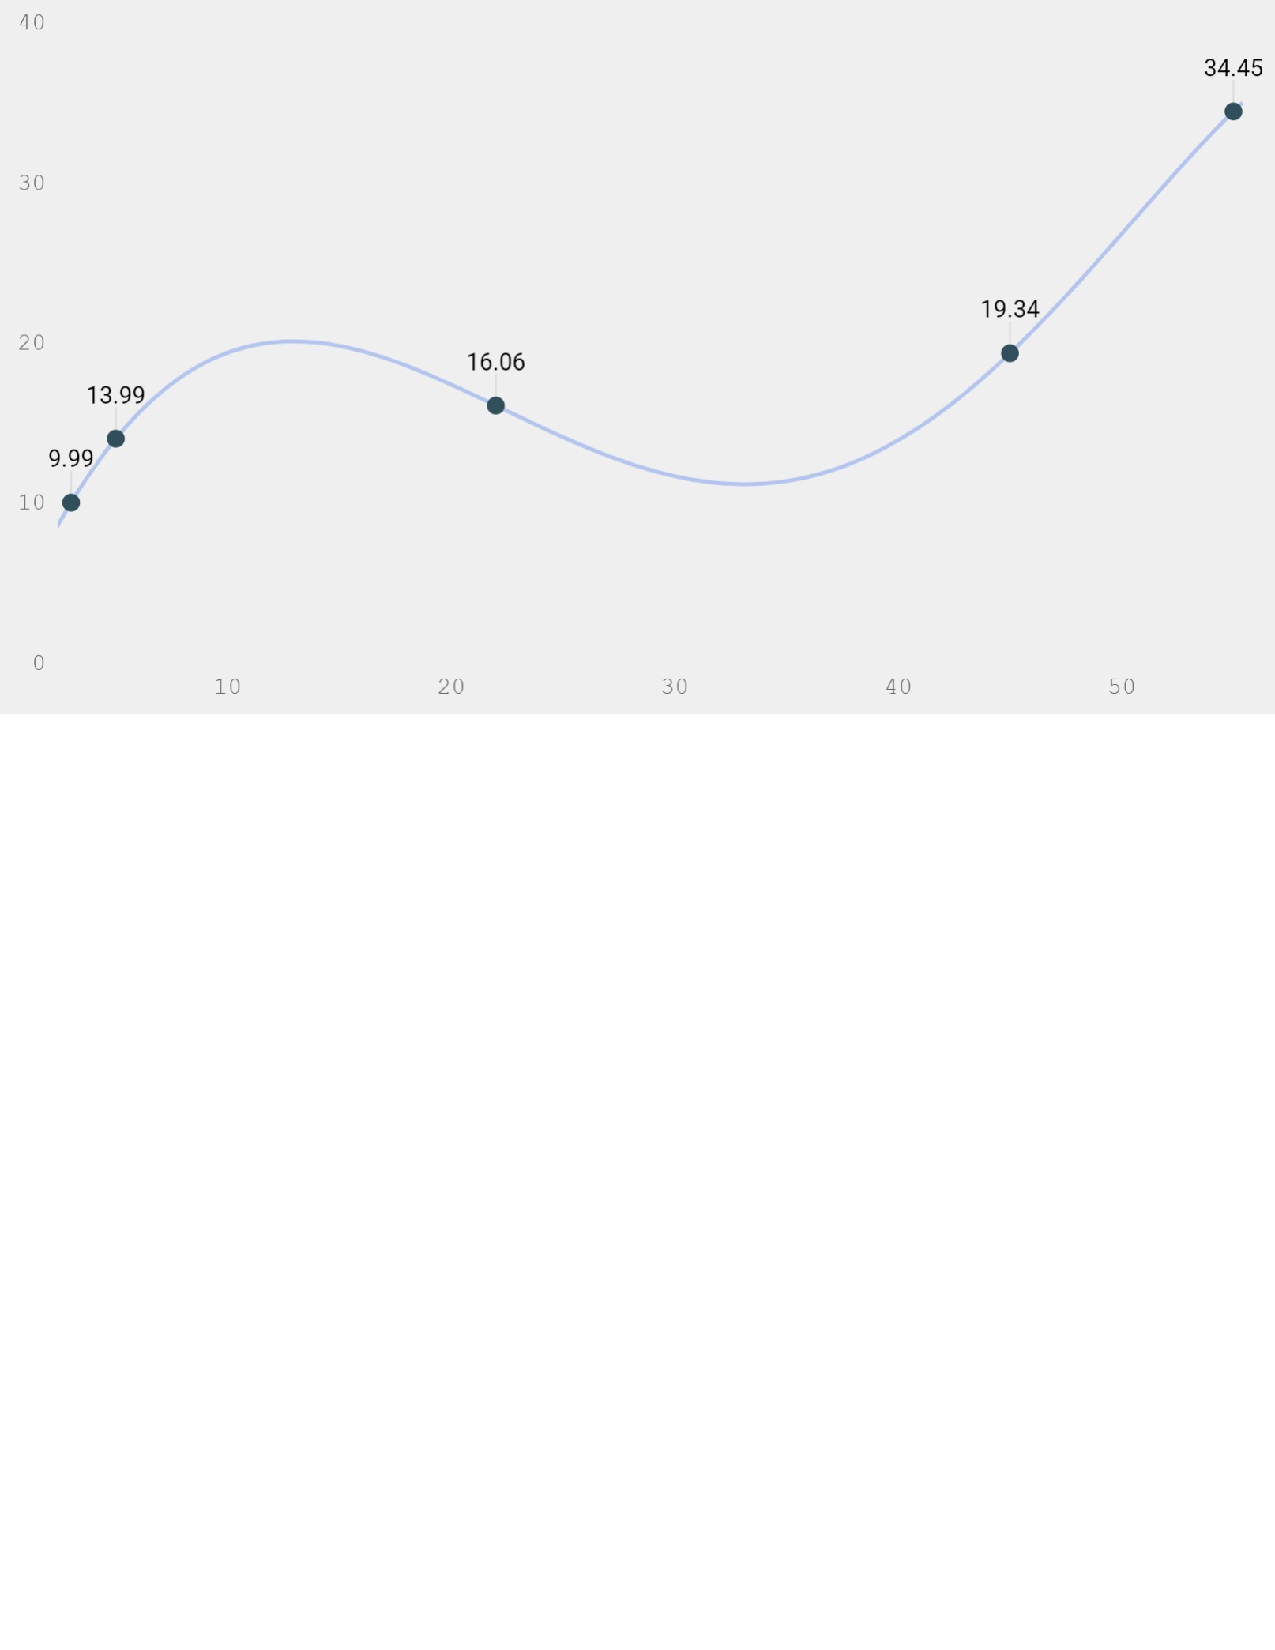
\includegraphics[width=11cm]{interpolate1}%
\vspace{-220pt}
\caption{A degree 5 interpolating polynomial passing through a dataset.}

\end{figure}

Polynomial interpolation involves the construction of a smooth continuous polynomial from a discrete set of data points; it permits the approximation of a function. Given $a = x_0 < x_1 < x_2 < \cdots < x_n = b$, which is a partition of the closed interval $[a, b]$. Polynomial interpolation is the process of finding a nth degree polynomial $p(x)$ that agrees with $f(x)$ at the points of the partition. Polynomial interpolation is a subclass of polynomial approximation in which the interpolating polynomial must pass through all of the data points \cite{LHK3}.

\begin{equation}
p\left(x\right) = f(x_i), \qquad \forall \ i = 0, 1,2, \cdots,n.
\end{equation}

The Weierstrass Approximation theorem confirms that, if given a continuous function on a closed interval, $f(x) \in C[a, b]$, then for each $\epsilon > 0$, there exists a polynomial $p(x)$ with the property that:

\begin{equation}
|f(x) - p(x)| < \epsilon, \qquad \forall \ x \in [a, b]
\end{equation}

Thus, polynomials can be used to approximate functions arbitrarily well. Polynomials have many desirable properties, including: that they are easy to evaluate, differentiate, and integrate.

\subsection{The Direct Method}
One of the most straightforward approaches to polynomial interpolation involves the use of the Vandermonde matrix, from henceforth the method will be referred to as the Direct method. Consider some nth degree polynomial \cite{LHK3}:

\begin{equation}
P_n\left(x\right) = a_0 + a_1x + a_2x^2 + \cdots + a_nx^n
\end{equation}

To construct the interpolating polynomial via the Direct method, the coefficients must be determined by solving the following linear system:

\begin{equation}
\begin{split} % Split into multiple lines.
&f_0 = a_0 + a_1x_0 + a_2x_0^2 + \cdots + a_nx_0^n \\
&f_1 = a_0 + a_1x_1 + a_2x_1^2 + \cdots + a_nx_1^n \\
&\hspace{0.3cm} \vdots \qquad \vdots \qquad \vdots \qquad \vdots \qquad \vdots \qquad \vdots \qquad \vdots \\
%\vdots \\ % \vdots
&f_n = a_0 + a_1x_n + a_2x_n^2 + \cdots + a_nx_n^n
\end{split}
\end{equation}

Now consider the matrix of monomials, $V$, the column vector of coefficients, $a$, and the column vector, $f$:

\begin{equation}
V = \begin{bmatrix}
1 & x_0 & x_0^2 & \cdots & x_0^n\\
1 & x_1 & x_1^2 & \cdots & x_1^n\\
\vdots & \vdots & \vdots & \vdots & \vdots\\
1 & x_n & x_n^2 & \cdots & x_n^n
\end{bmatrix}
\end{equation}

% TEST
\begin{equation}
a = \begin{bmatrix} a_0\\a_1\\ \vdots\\a_n\end{bmatrix}
\quad % horizontal spacing
f = \begin{bmatrix} f_0\\f_1\\ \vdots\\f_n\end{bmatrix}
\end{equation}
%

The matrix $V$ is called the Vandermonde matrix and solving the following system will yield the desired coefficient vector which describes the interpolating polynomial:
\begin{equation}\label{DirectEq}
Va = f
\end{equation}

There are several methods from linear algebra for solving this system including: Eigenvalue Decomposition, QR Decomposition, Singular Value Decomposition (SVD), Gaussian Elimination, and solving the system with the inverse matrix. Each method employs a novel strategy which may be more or less computationally efficient in terms of solving a given system. Having to solve a system of equations can be done in $O(n^2)$ arithmetic operations best case; however, the general case is $O(n^3)$ operations. These systems can be ill-conditioned, tiny changes in the $x's$ can generate large changes in the solution.

\subsection{Lagrange Interpolation}

Consider some dataset of size $n$: $\{x_i,y_i\}^n_i=0$ where $n \geq 1$, there exists polynomials $L_k \in P(x),$ $k = 0,1,2,\cdots, n$. The polynomial \cite{LHK3}:

\begin{equation}
p_n(x) = \sum_{k=0}^{n} L_k(x)\cdot y_k
\end{equation}

Satisfies the interpolation conditions:

\begin{equation}
p_n(x_i) = y_i, i = 0, 1, 2, \cdots, n.
\end{equation}

And $L_k$ is defined as:

\begin{equation}
L_k(x) = \prod_{0<i<n;\ i \ne k} \frac{x - x_i}{x_k - x_i}
\end{equation}

\subsection{Hermite Interpolation}

Hermite interpolation extends the idea of Lagrange interpolation by requiring the derivative values at the interpolation points. For the datasets: $\{y_i\}^n_{i=0}$ and $\{z_i\}^n_{i=0}$ corresponding to the dataset $\{x_i\}^n_{i=0}$ with $n \geq 0$, we need to find a polynomial $p_{2n+1} \in P_{2n+1}$ \cite{LHK4}.

\begin{equation} \label{Hconstraints}
p_{2n+1}(x_i) = y_i, p'_{2n+1}(x_i) = z_i, \qquad i = 0, 1, 2, \cdots, n.
\end{equation}

To satisfy the constraints imposed by \eqref{Hconstraints} two new quantities are defined:

\begin{equation} \label{Hkeq}
H_{k}(x) = [L_k(x)]^2\cdot (1 - 2L'_k(x_k)(x-x_k)),
\end{equation}

\begin{equation} \label{Kkeq}
K_{k}(x) = [L_k(x)]^2\cdot (x-x_k)
\end{equation}

The Hermite polynomial takes its final form with:
\begin{equation} \label{hermiteEq}
p_{2n+1}(x) = \sum_{k=0}^{n}[H_{k}(x)\cdot y_k + K_{k}(x)\cdot z_k]
\end{equation}

\subsection{Chebyshev Nodes}
The Chebyshev nodes are a set of real numbers representing the roots of the Chebyshev polynomials of the first kind. Chebyshev polynomials of the first kind can be obtained from the recurrence relation \cite{LHK5}:

\begin{equation}
\begin{split} % Split into multiple lines.
&T_0(x) = 1\\
&T_1(x) = x\\
&T_{n + 1}(x) = 2x \cdot T_n(x) - T_{n - 1}(x)
\end{split}
\end{equation}

For some natural number $i$, the nodes in the interval $(-1, 1)$ are:

\begin{equation} \label{cnode1}
x_j = cos(\frac{2j - 1}{2i}\pi), \qquad j = 1, 2, \cdots, n.
\end{equation}

This formula can be generalized to any interval $[a, b]$ via an affine transformation \cite{SGW}:
\begin{equation} \label{cnode1}
x_j = cos(\frac{2j - 1}{2i}\pi)\cdot \frac{(b-a)}{2} + \frac{(b+a)}{2}, \qquad j = 1, 2, \cdots, n.
\end{equation}

These nodes can be used as opposed to $n$ equally spaced points to create an interpolating polynomial which mitigates Runge's phenomenon. Runge's phenomenon is the tendency for high degree interpolating polynomials to start violently oscillating near the endpoints; consequently, generating a large amount of error.

\clearpage
\newpage
\section*{Figures}

\subsection{$f\left(x\right) = Sin(x)$}
\vspace{5pt}
% Old way of including figures:
%\vspace{-12em} % I can control the vertical spacing this way.
%\hskip -7em
%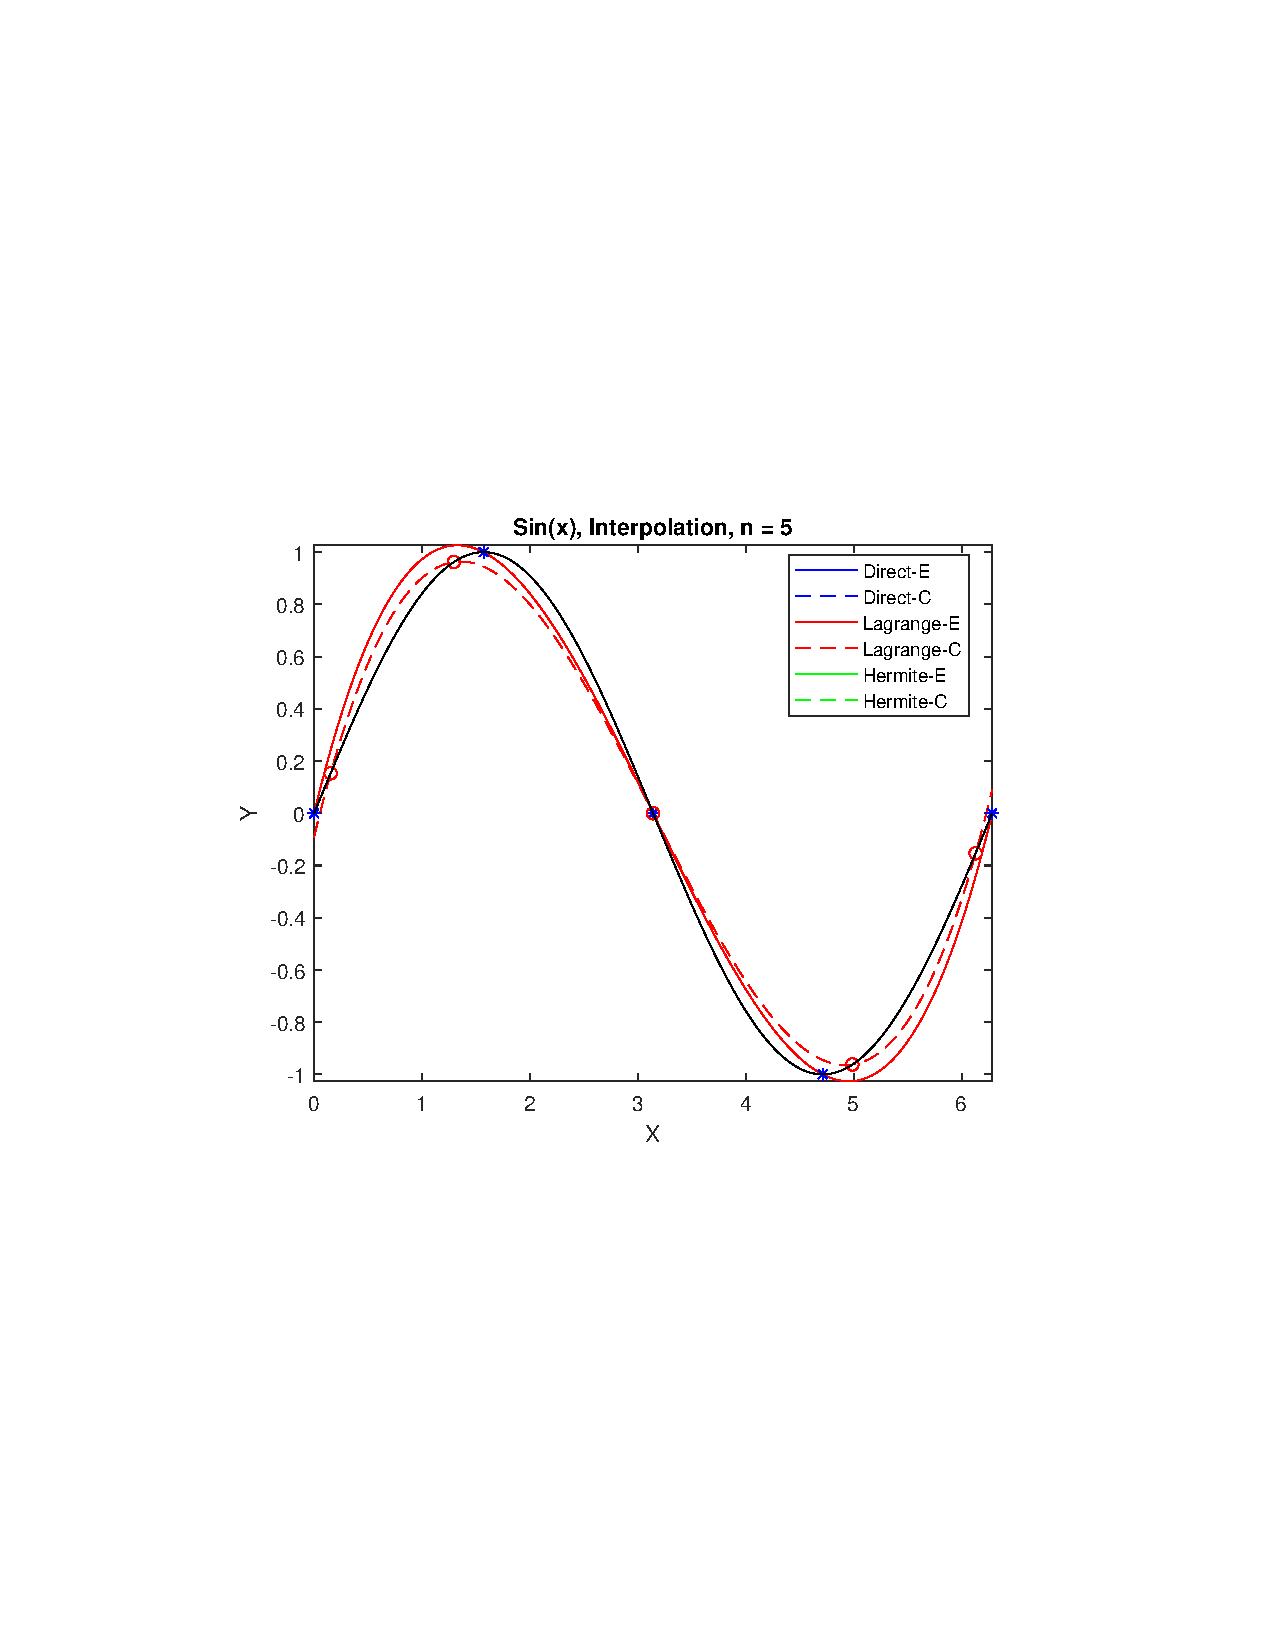
\includegraphics[width=0.8\linewidth]{function1_5} %\hspace{0.001\textwidth}
%\hskip -10em
%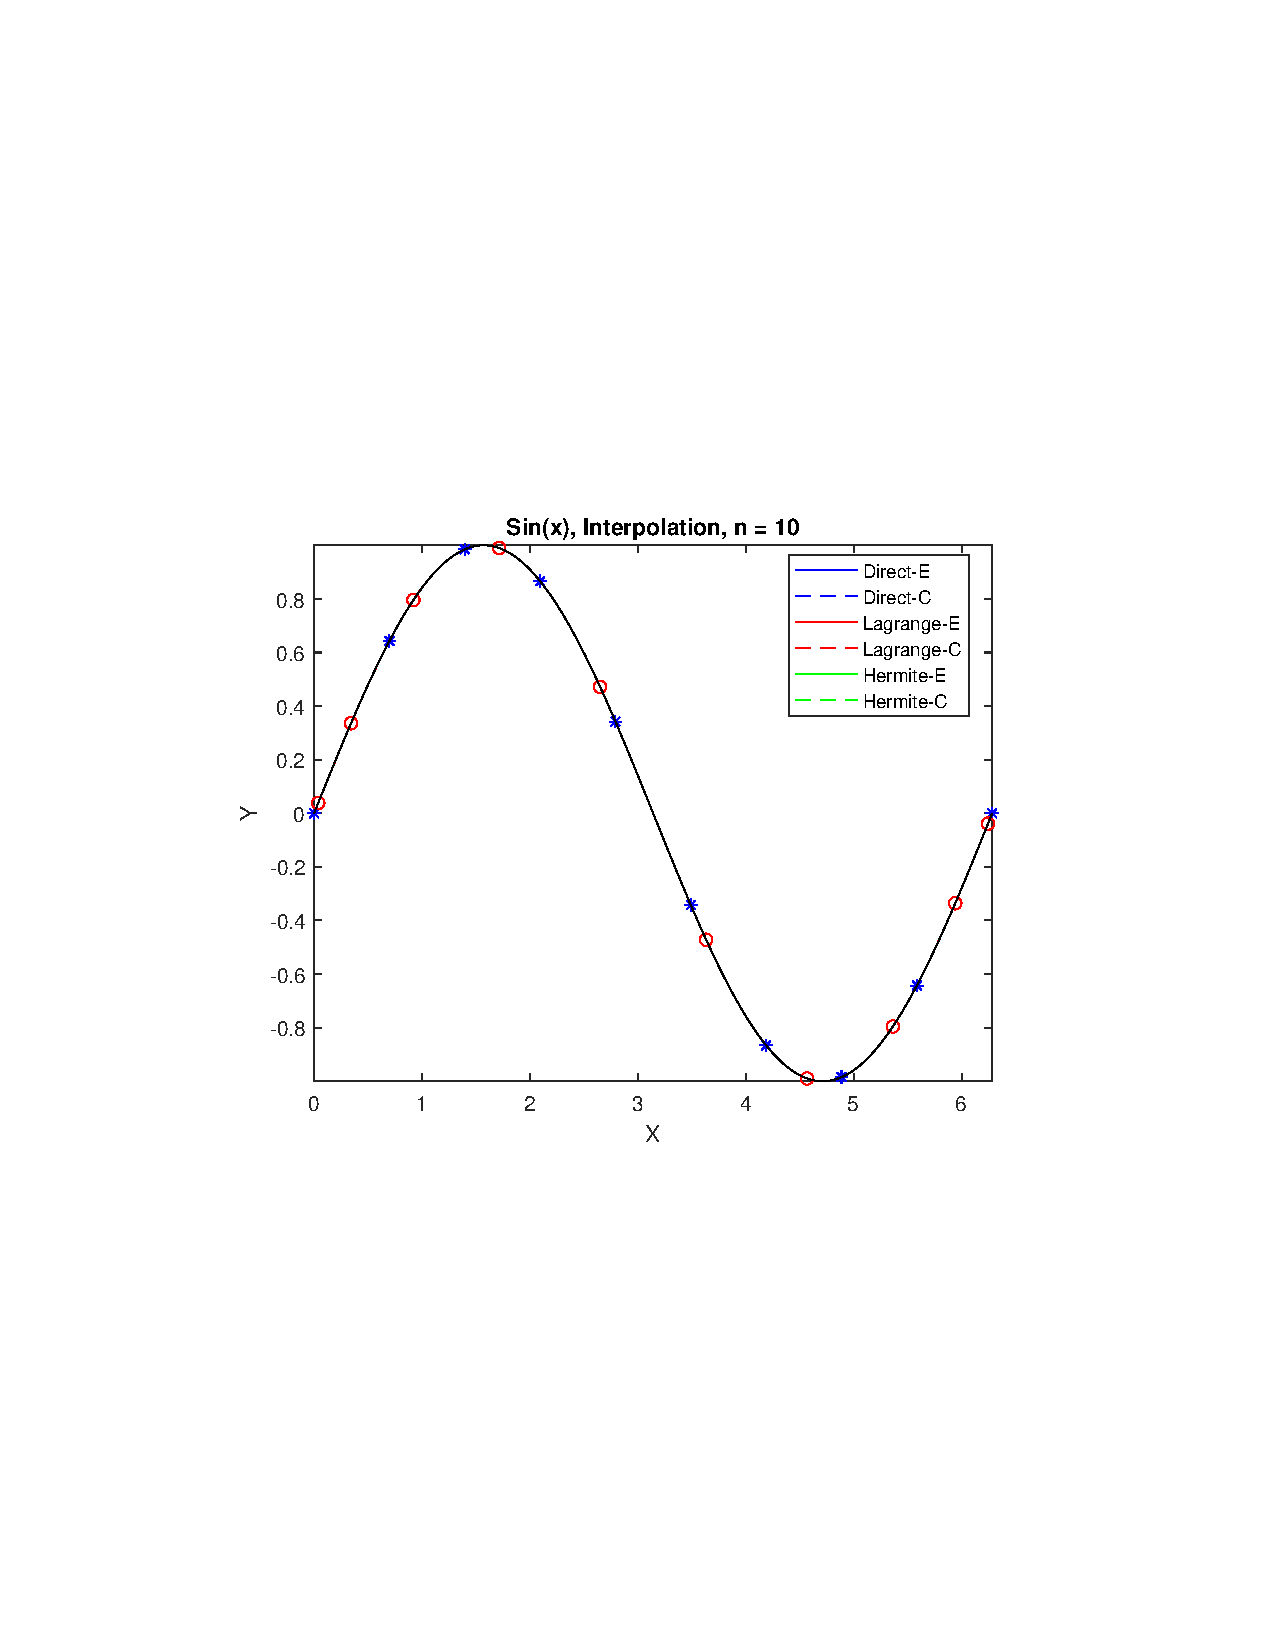
\includegraphics[width=0.8\linewidth]{function1_10}
%\newline
%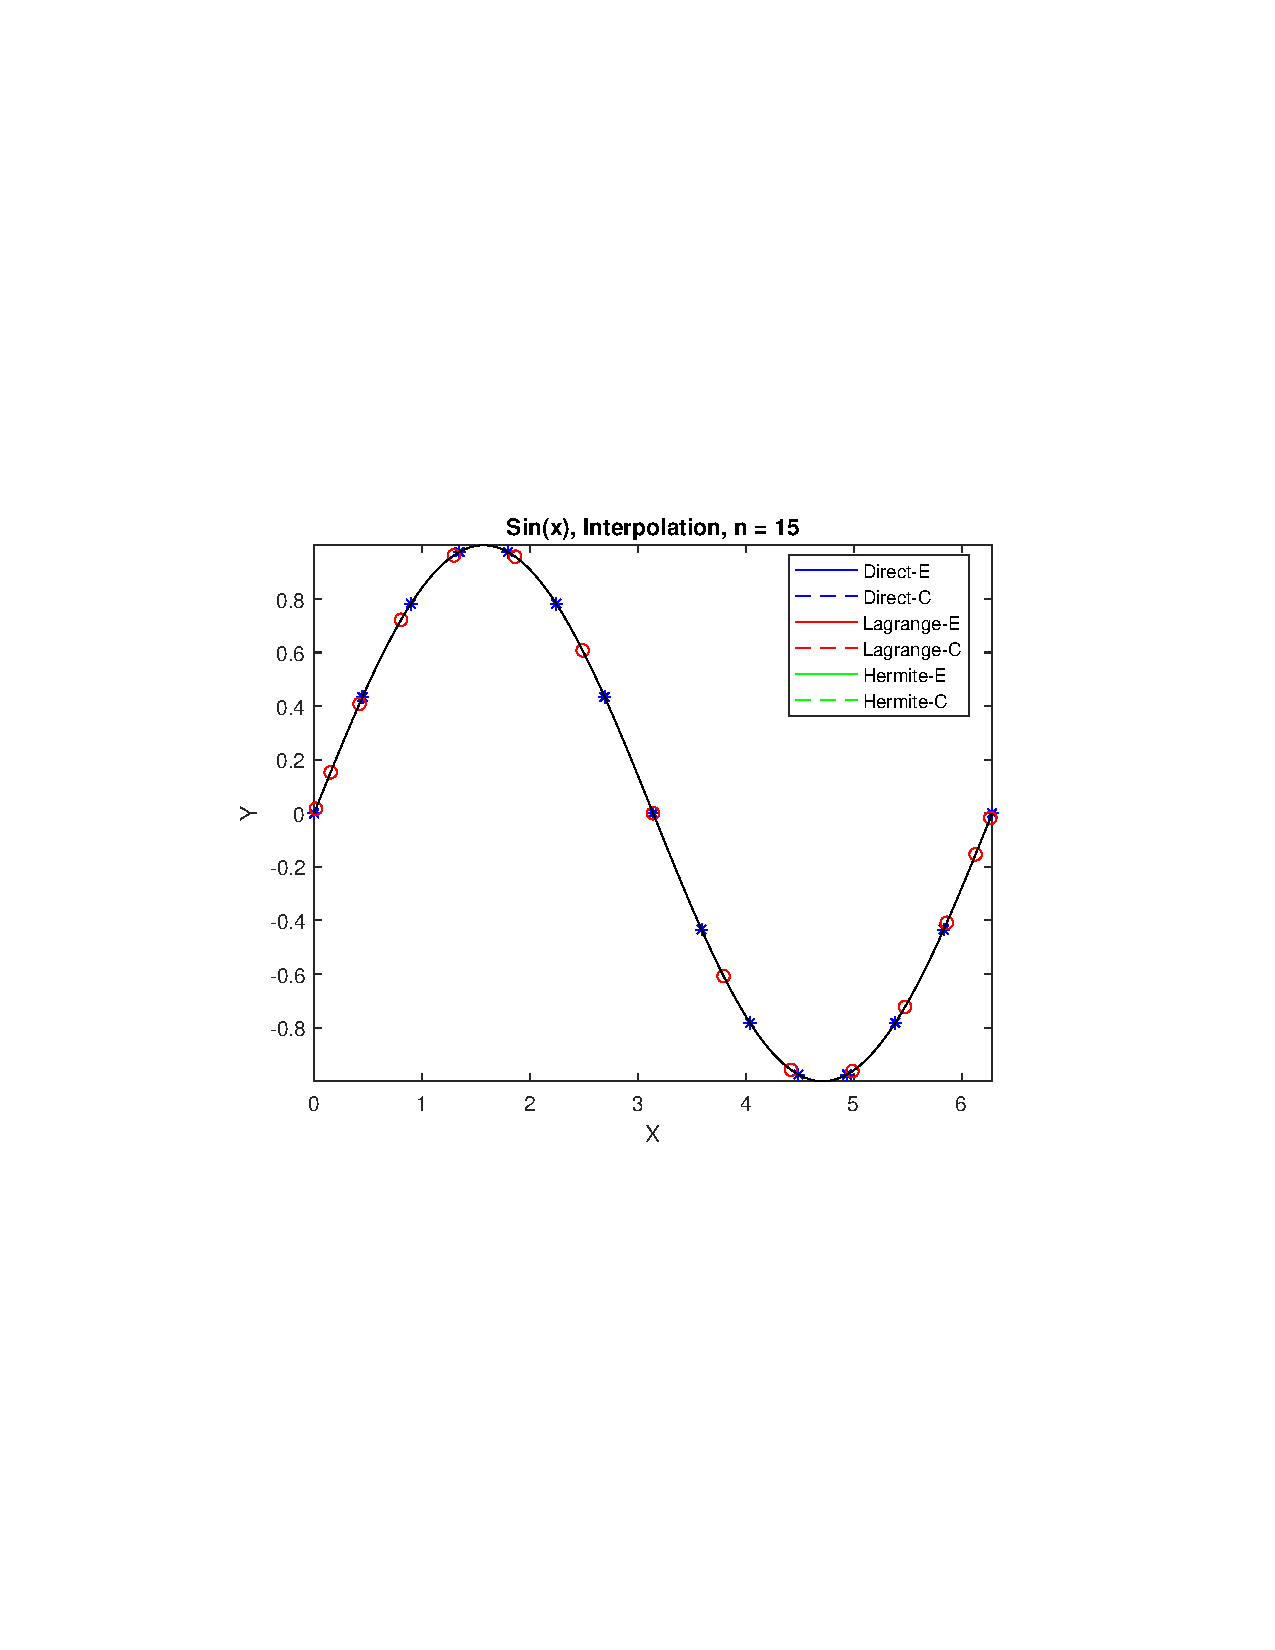
\includegraphics[width=0.8\linewidth]{function1_15}

% Breaking Sin(x) Figures up into sub figures: 3 rows of 2 & 2 rows of 2.

\begin{figure}[h]
\setlength{\lineskip}{-205pt}
\centering
\vspace{-125pt} % I can control the vertical spacing this way.
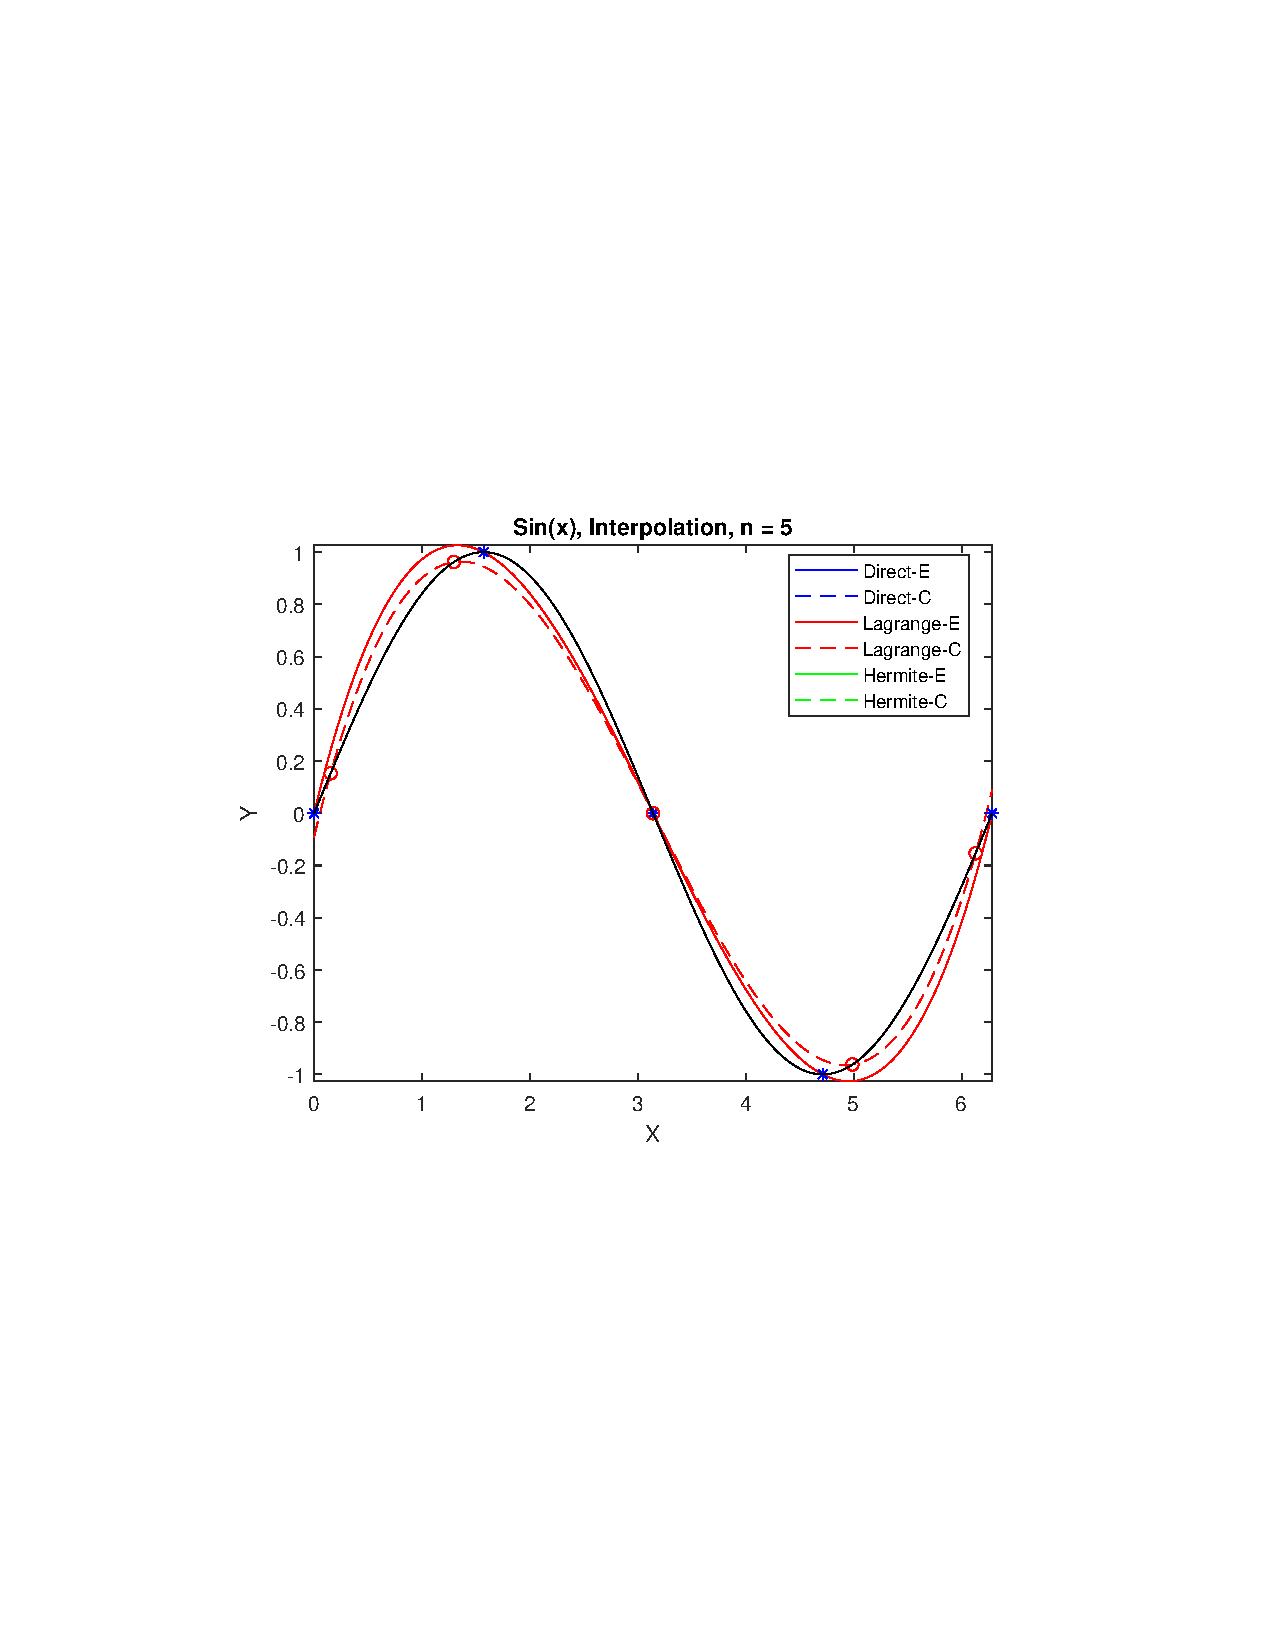
\includegraphics[width=9cm]{function1_5}%
\hskip -6em
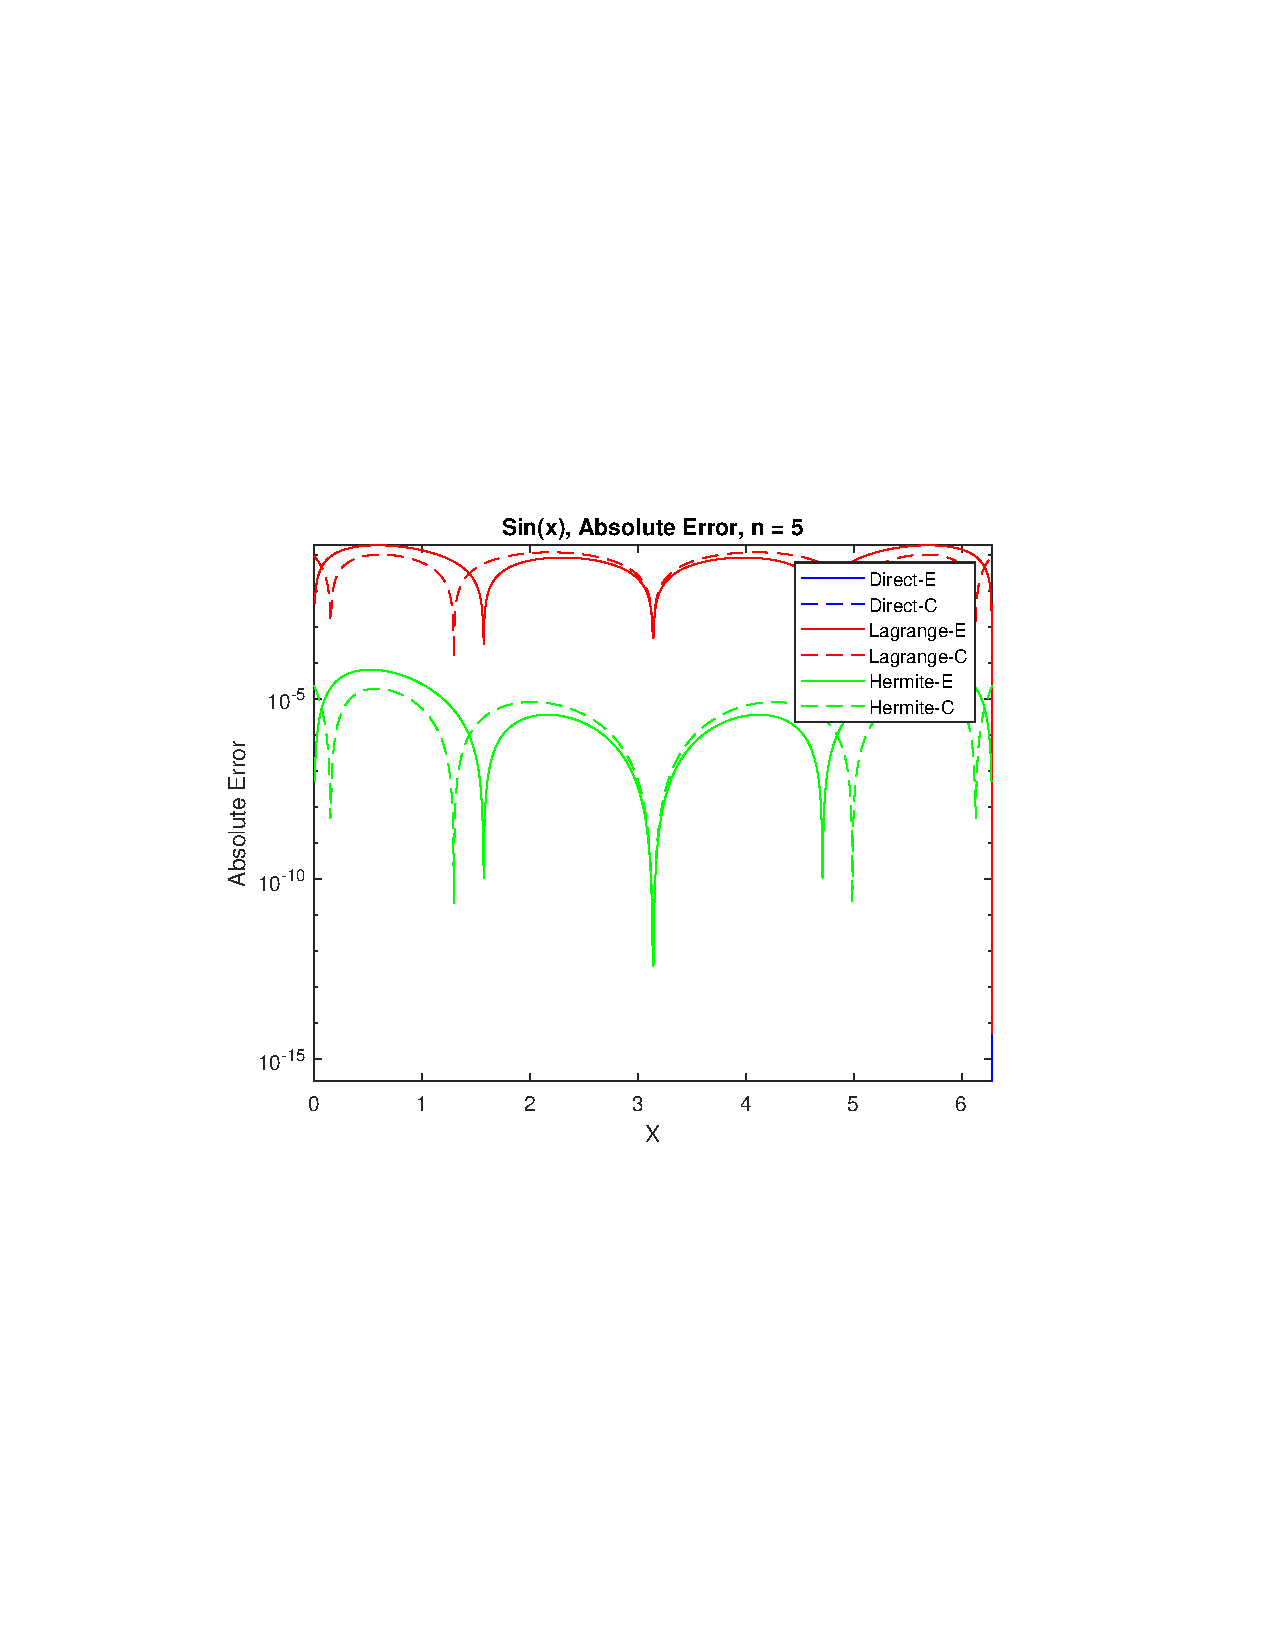
\includegraphics[width=9cm]{function1_absoluteError_5}\\
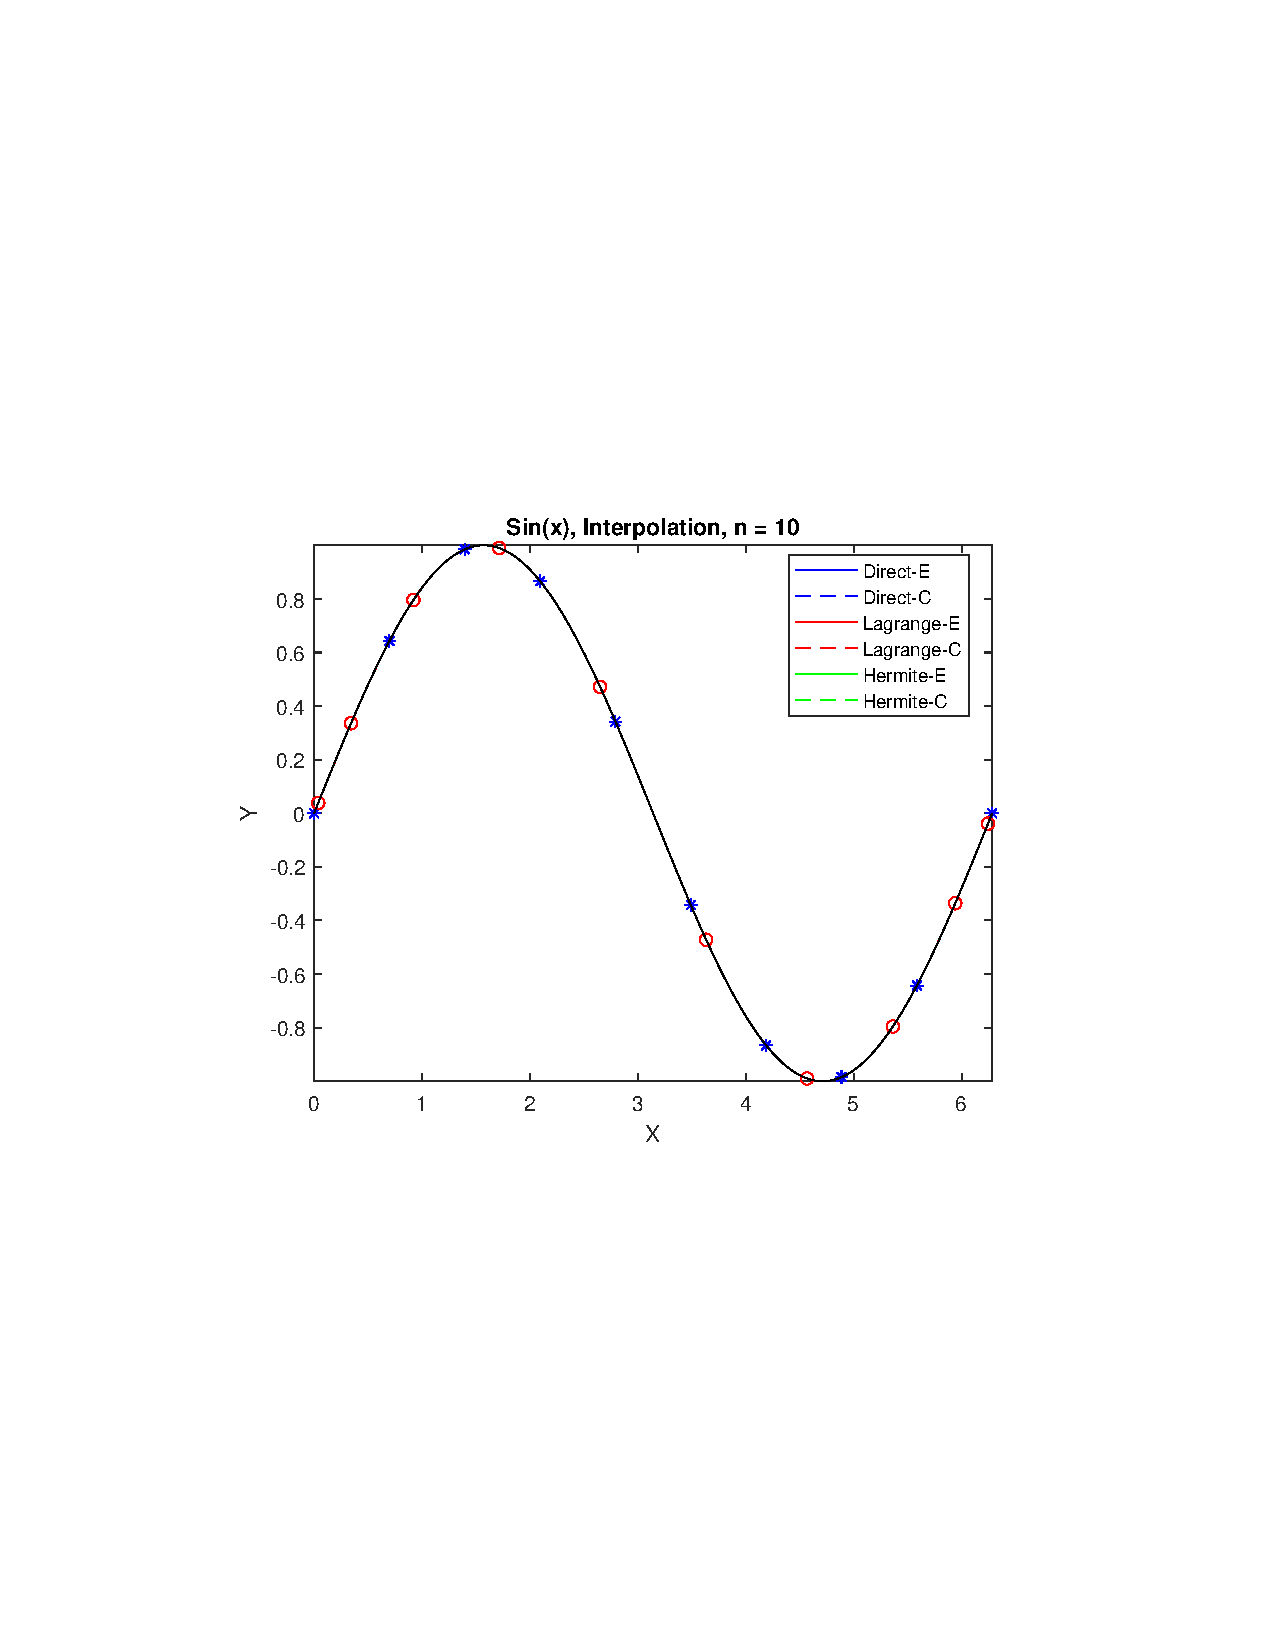
\includegraphics[width=9cm]{function1_10}%
\hskip -6em
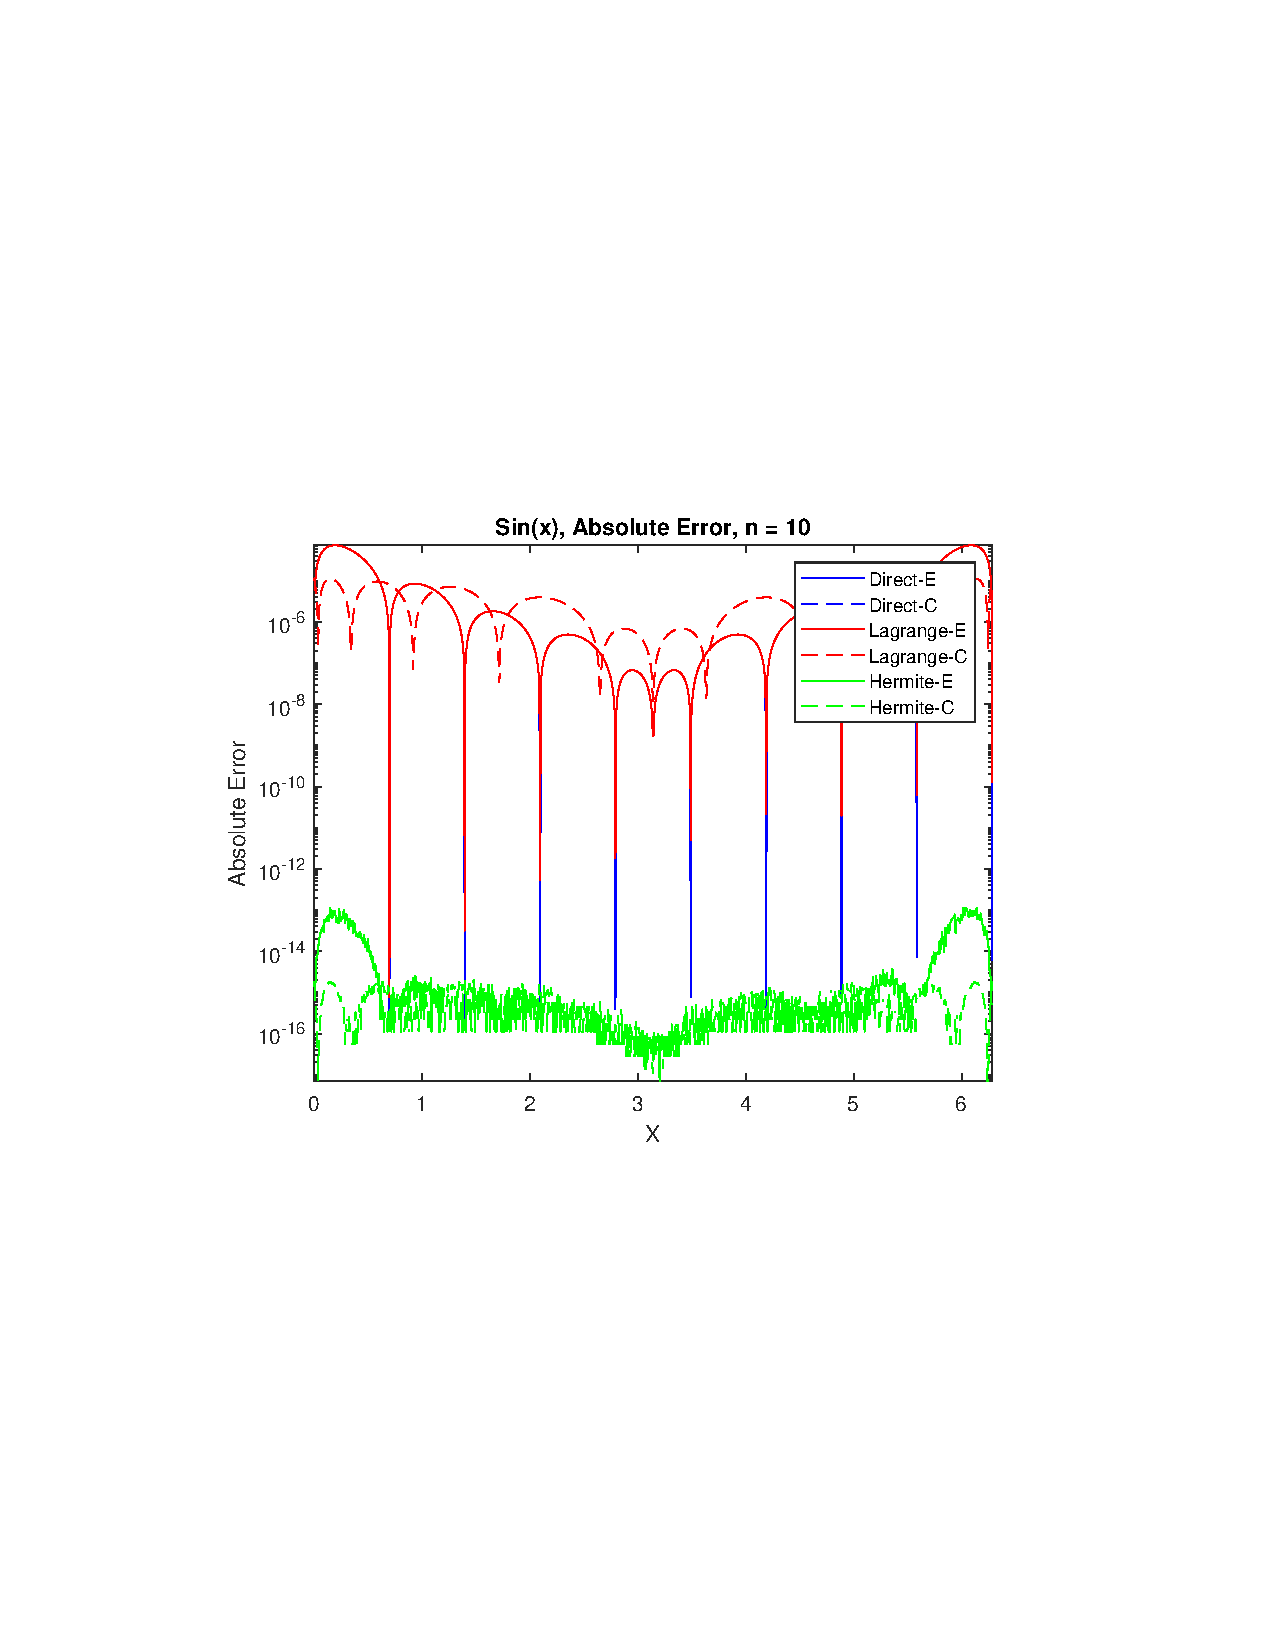
\includegraphics[width=9cm]{function1_absoluteError_10}\\
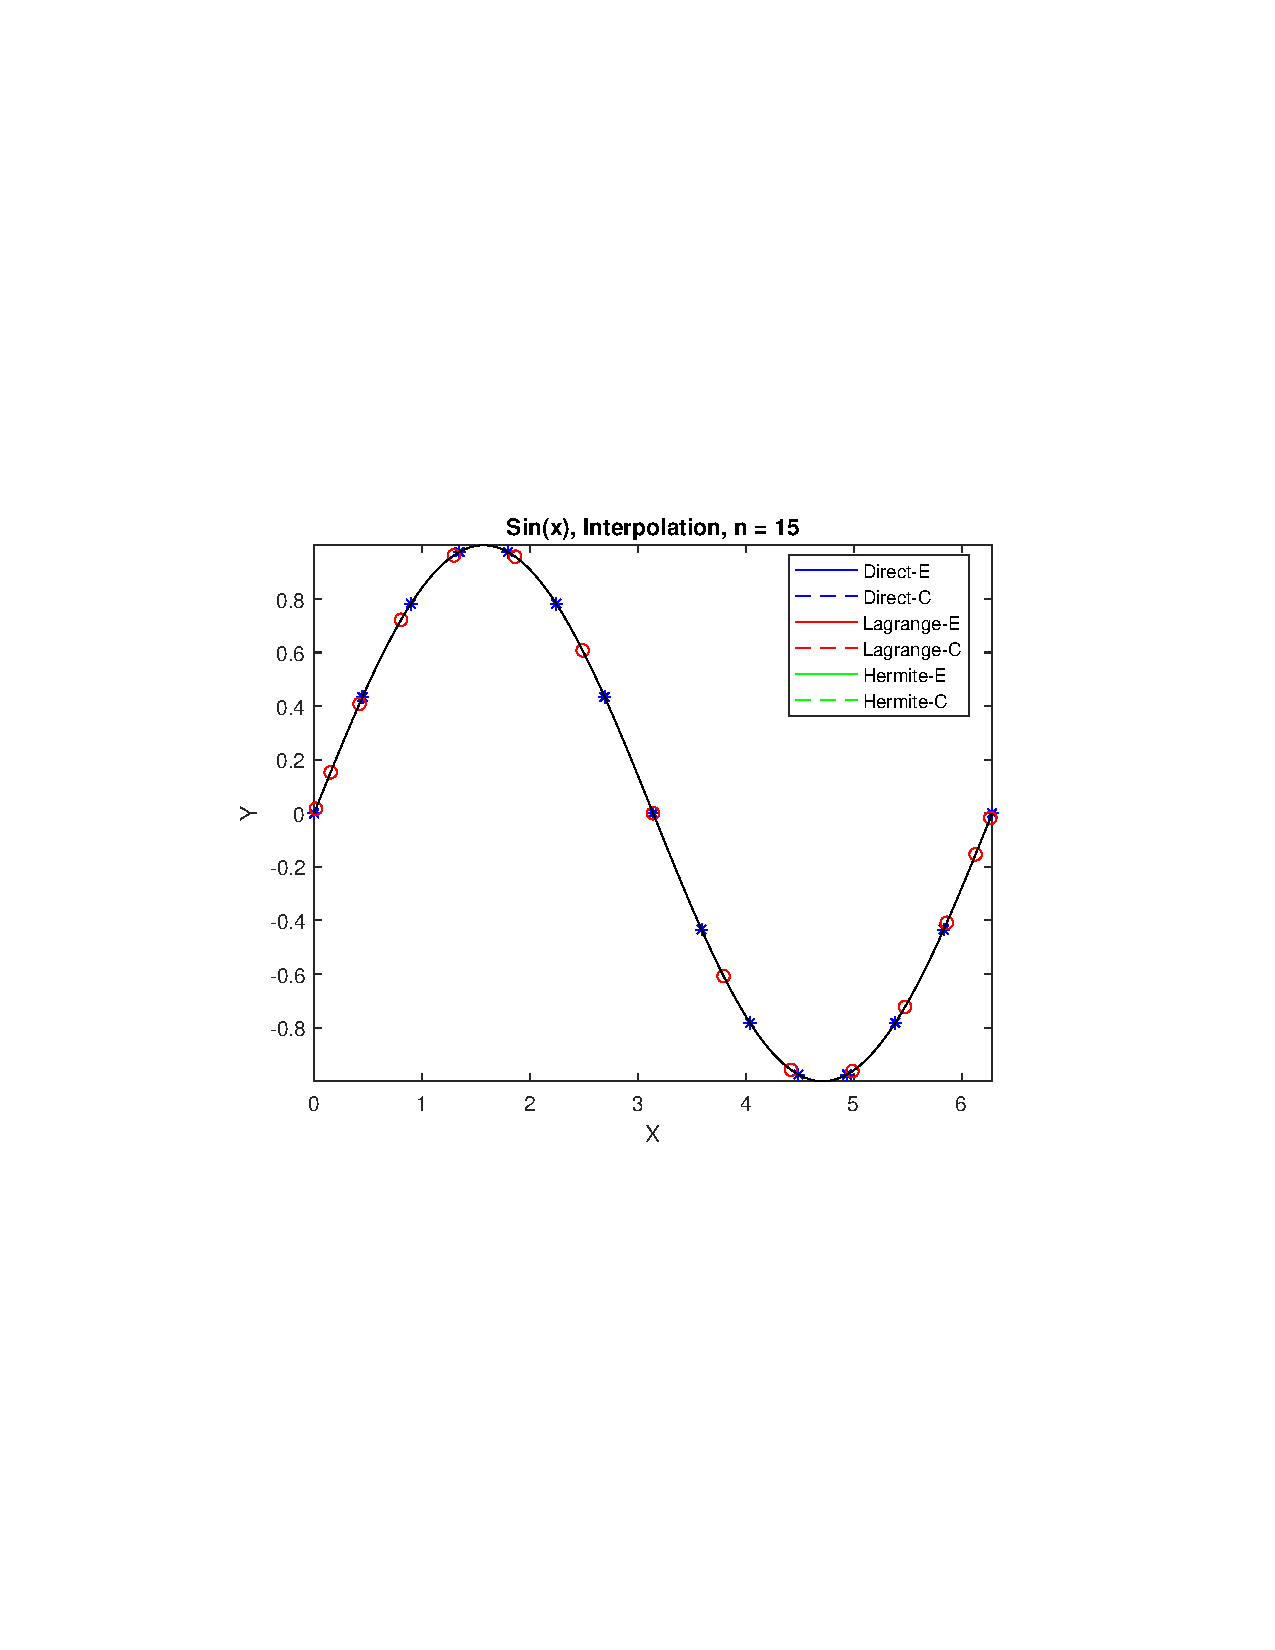
\includegraphics[width=9cm]{function1_15}%
\hskip -6em
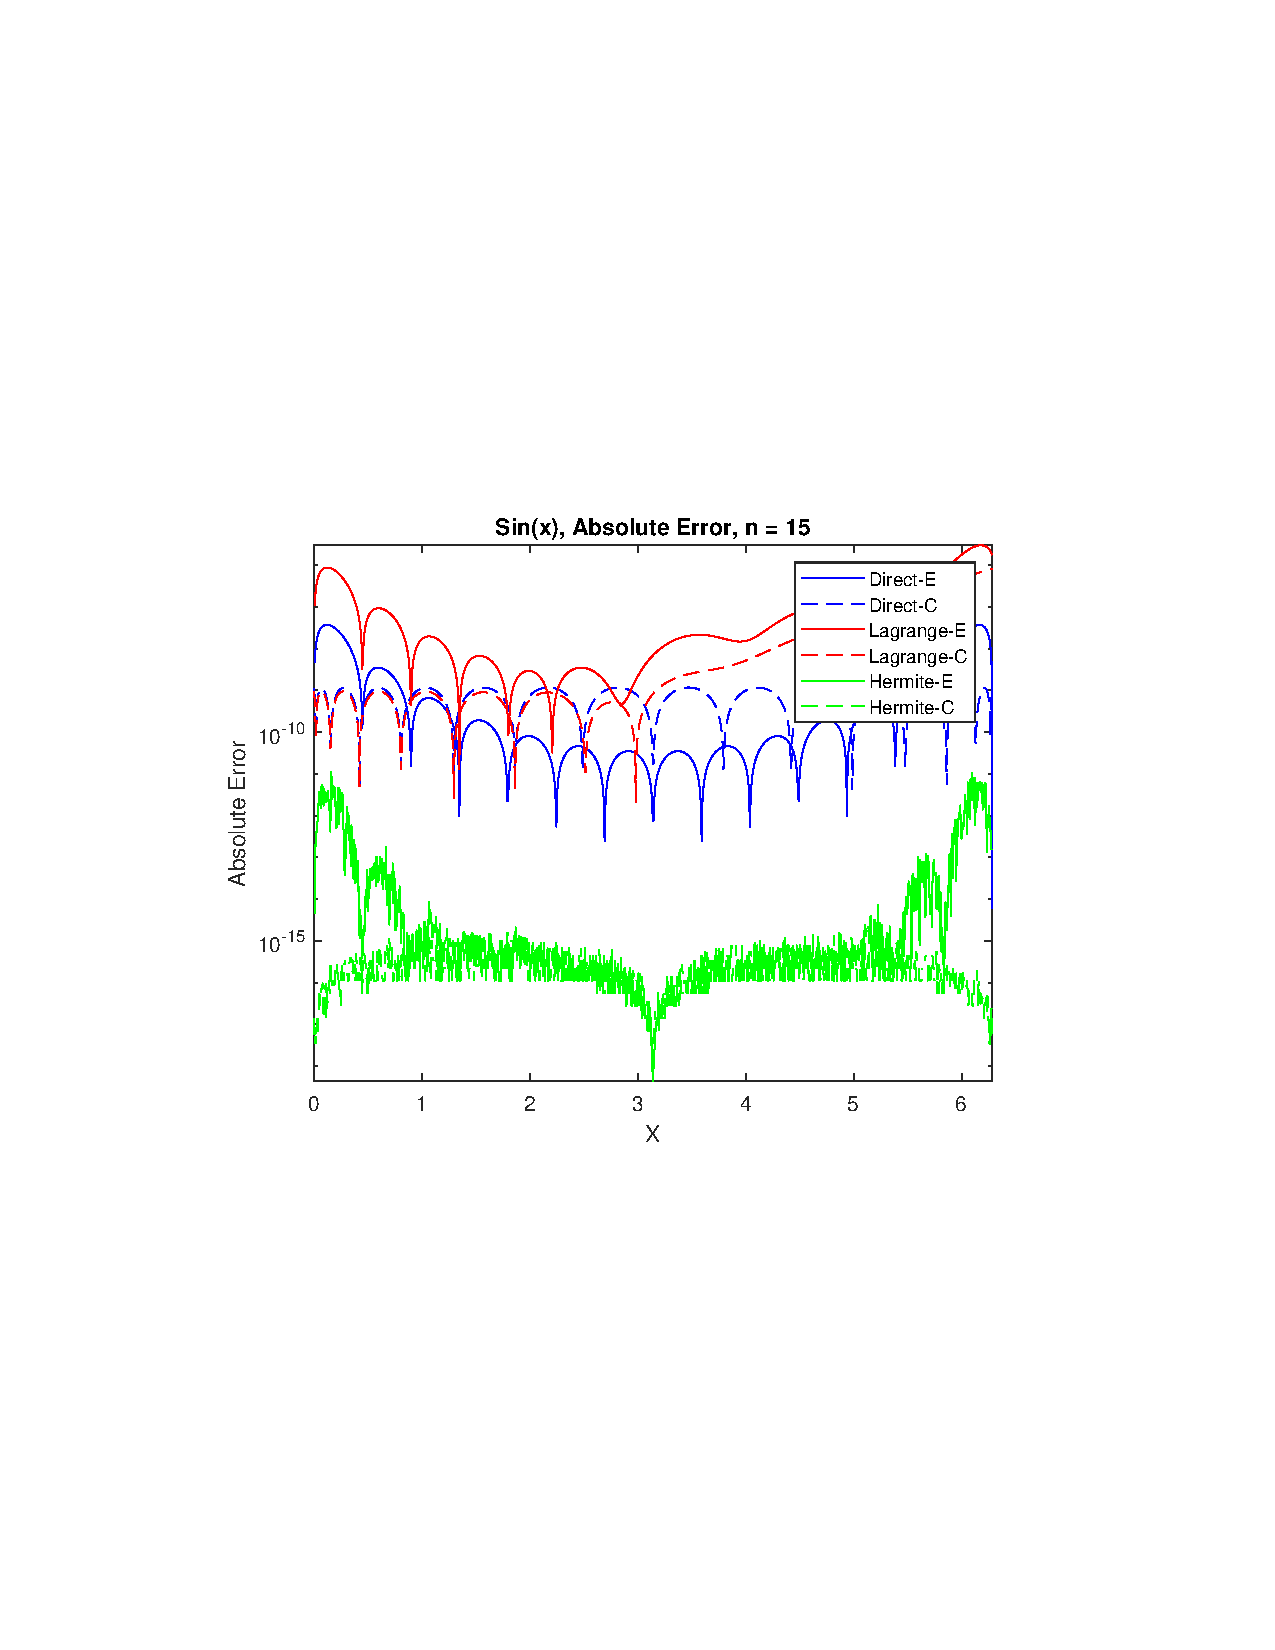
\includegraphics[width=9cm]{function1_absoluteError_15}\\
\end{figure}


\vspace{-100pt} % I can control the vertical spacing this way.
\begin{figure}[htp]
\setlength{\lineskip}{-170pt}
%\centering
\vspace{-170pt} % I can control the vertical spacing this way.
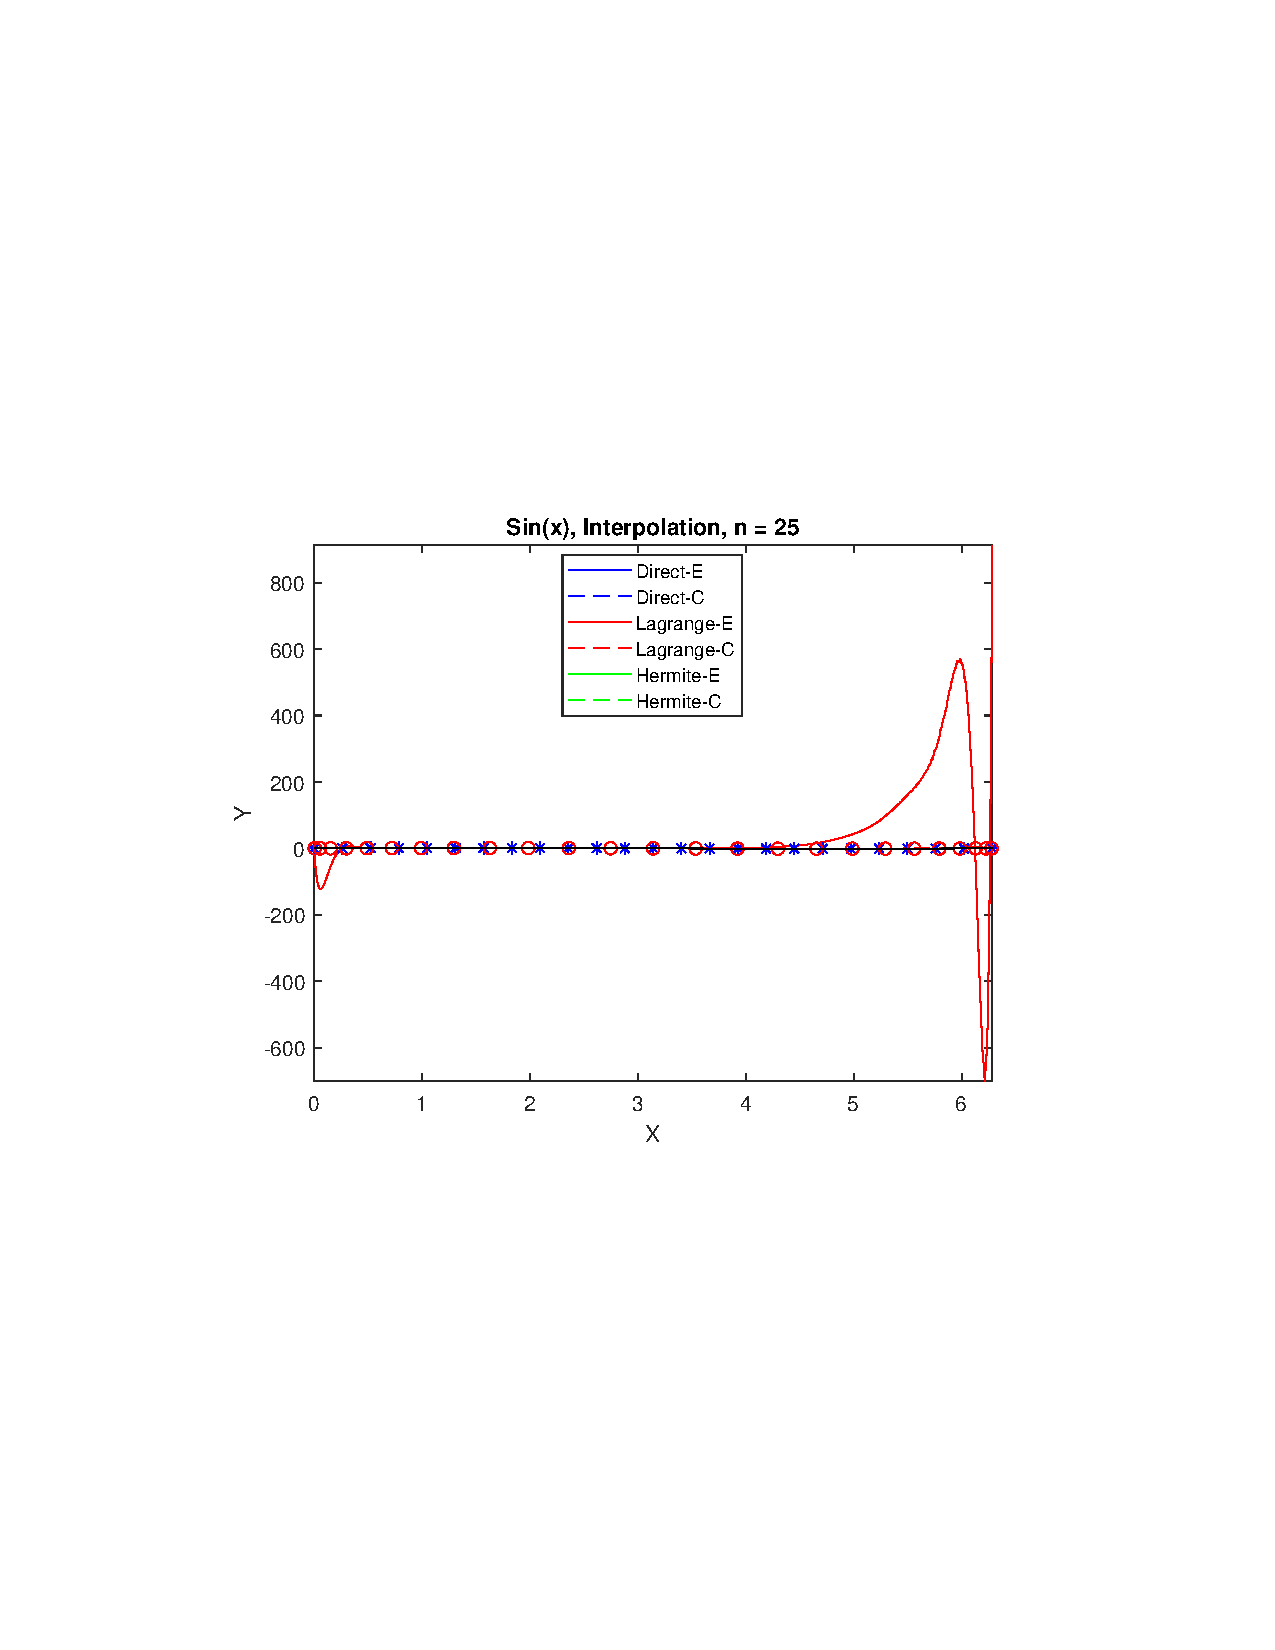
\includegraphics[width=8cm]{function1_25}%
\hskip -3em
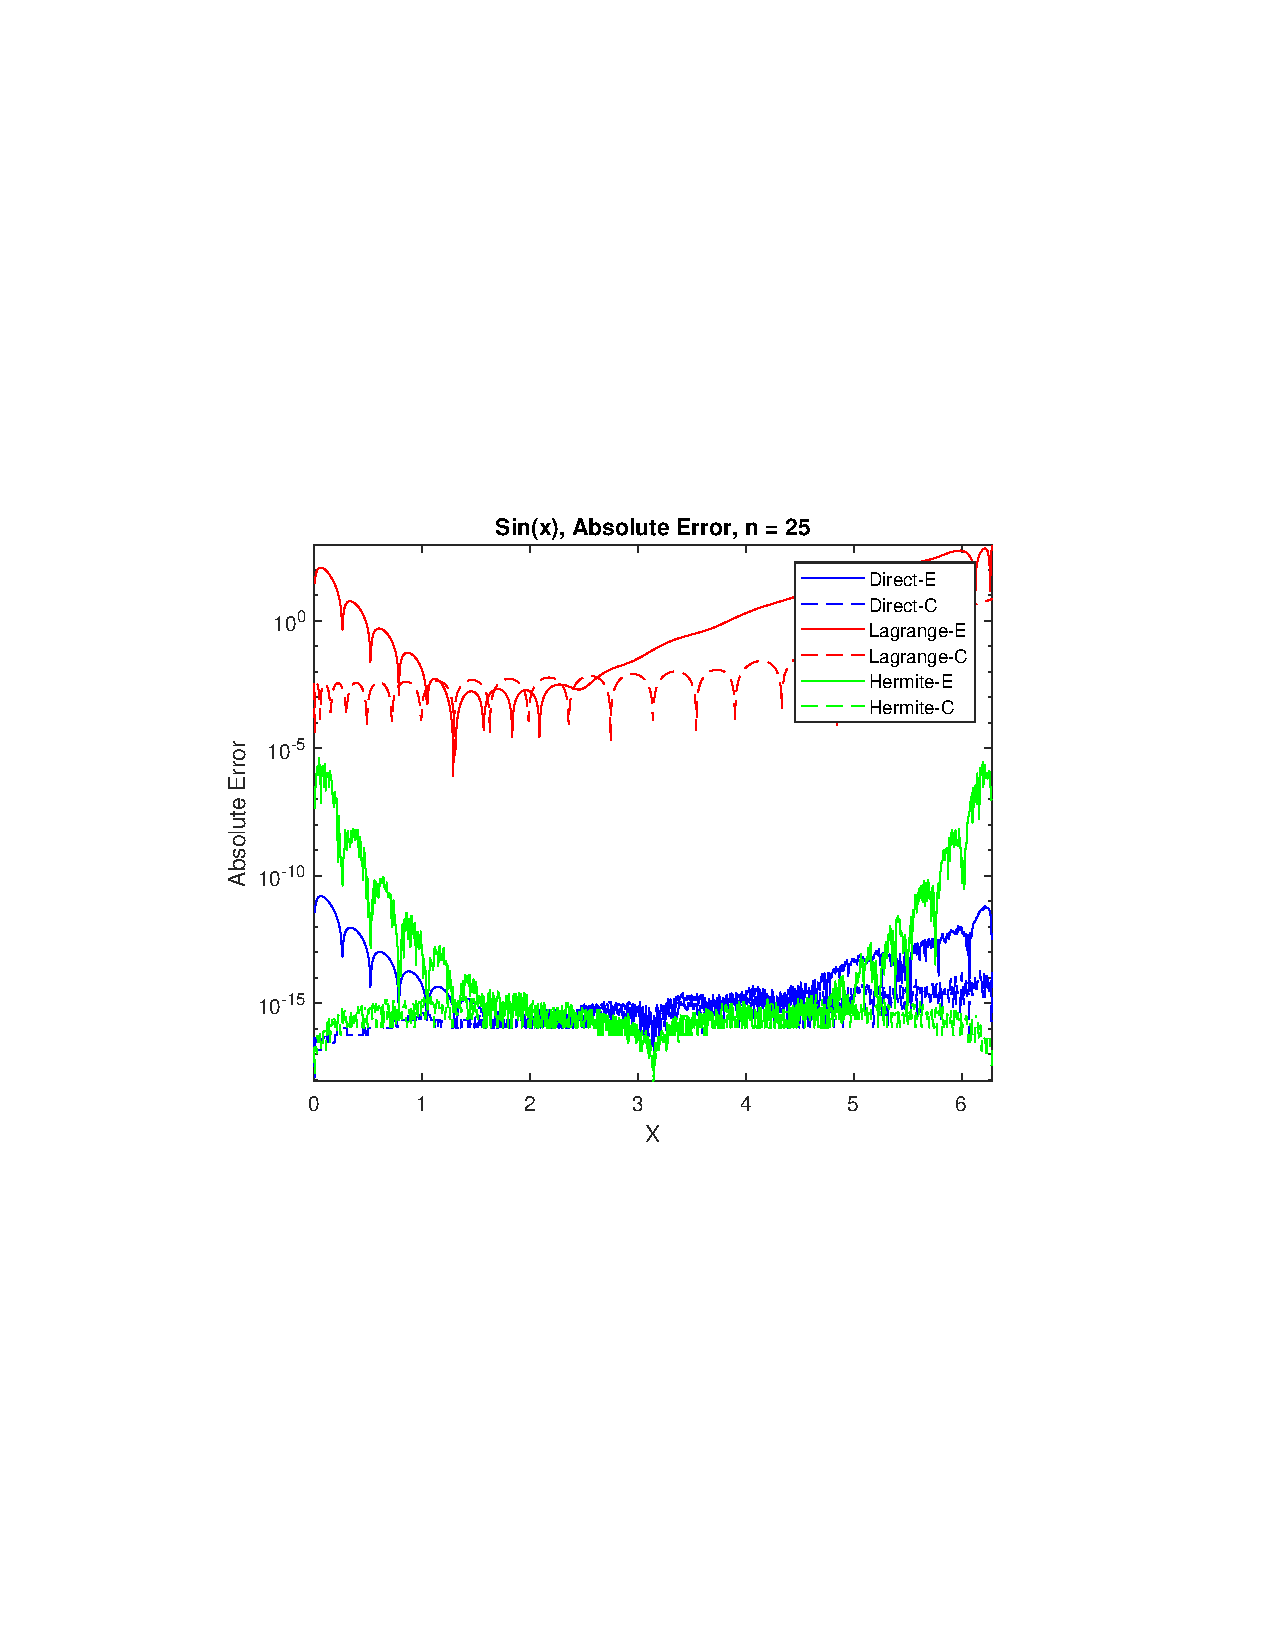
\includegraphics[width=8cm]{function1_absoluteError_25}\\
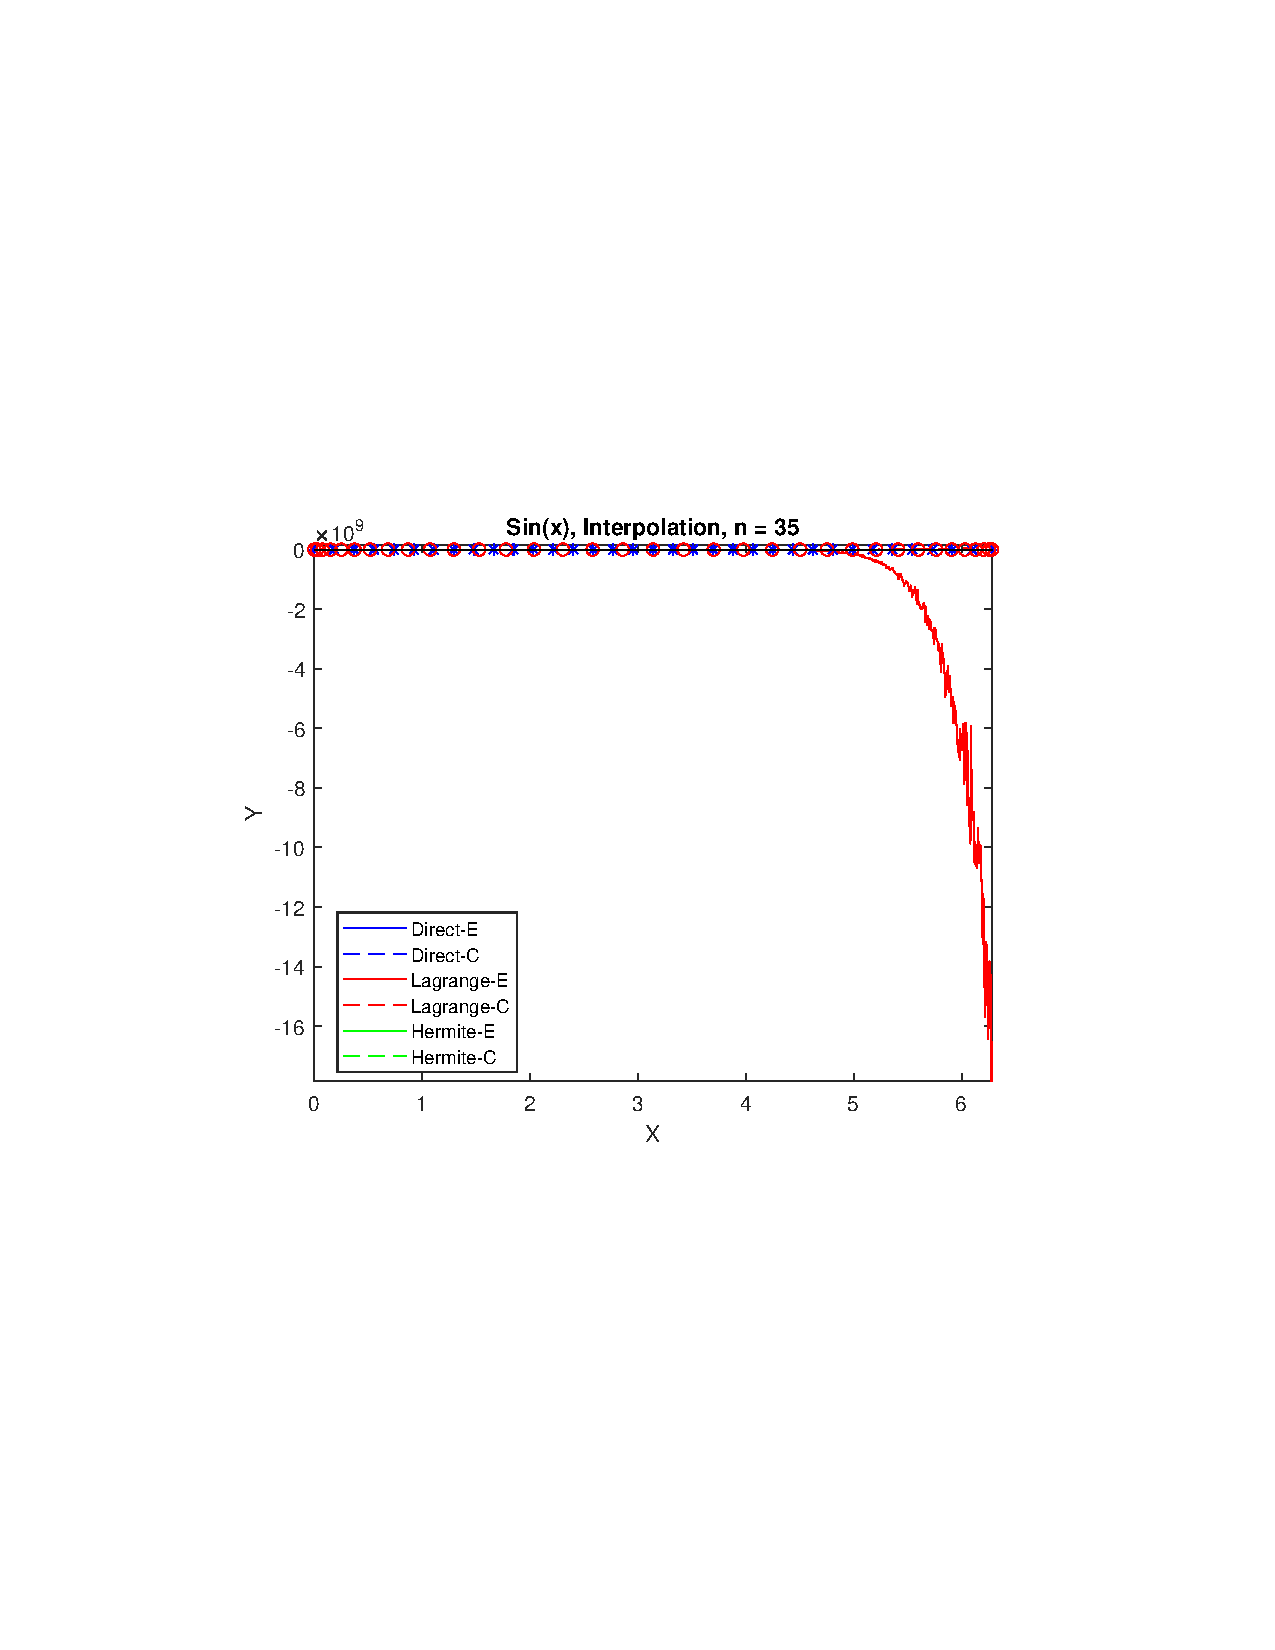
\includegraphics[width=8cm]{function1_35}
\hskip -3em%
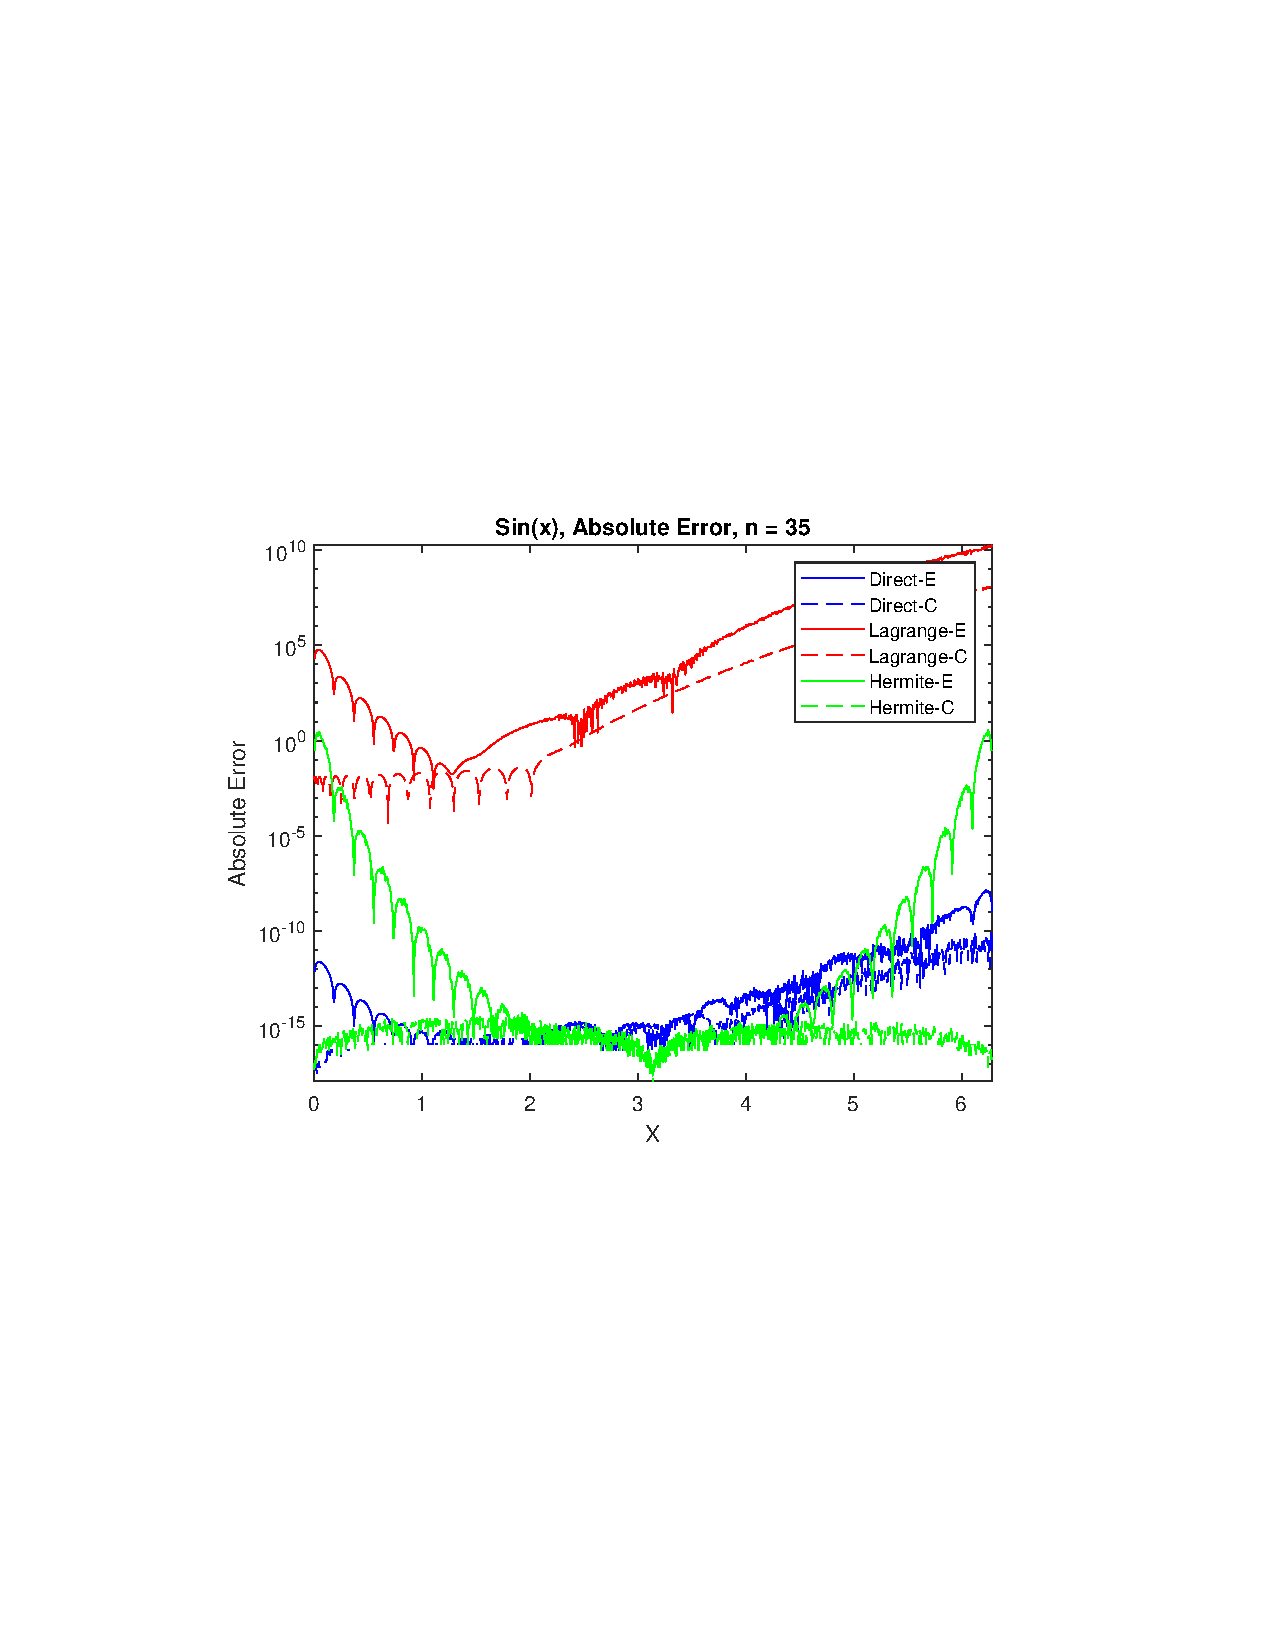
\includegraphics[width=8cm]{function1_absoluteError_35}\\

\vspace{-100pt} % I can control the vertical spacing this way.
\caption{Approximation \& error analysis of $Sin(x)$.}
\end{figure}


\clearpage
\newpage
\subsection{$f\left(x\right) = Sin(5x)$}
% Breaking Sin(5x) Figures up into sub figures: 3 rows of 2 & 2 rows of 2.
\vspace{25pt}
\begin{figure}[htp]
\setlength{\lineskip}{-205pt}
\centering
\vspace{-125pt} % I can control the vertical spacing this way.
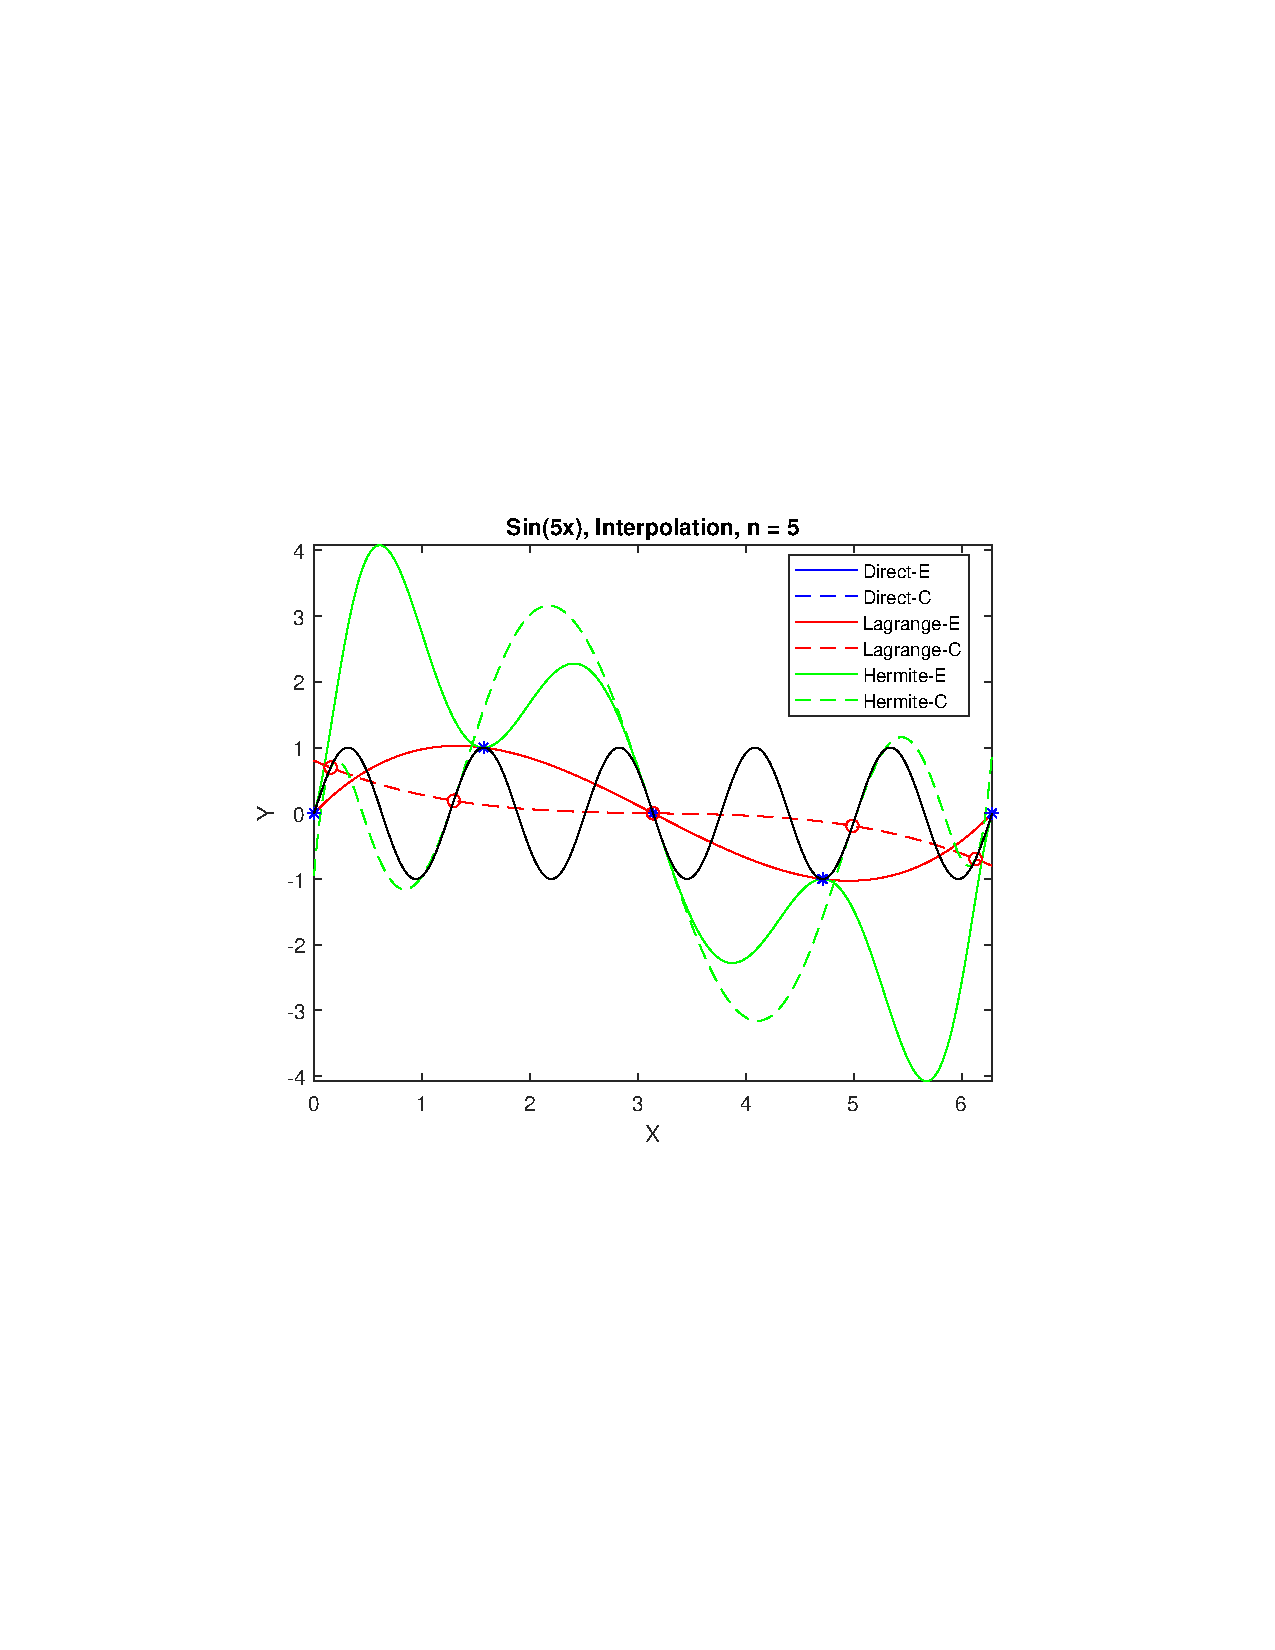
\includegraphics[width=9cm]{function2_5}%
\hskip -6em
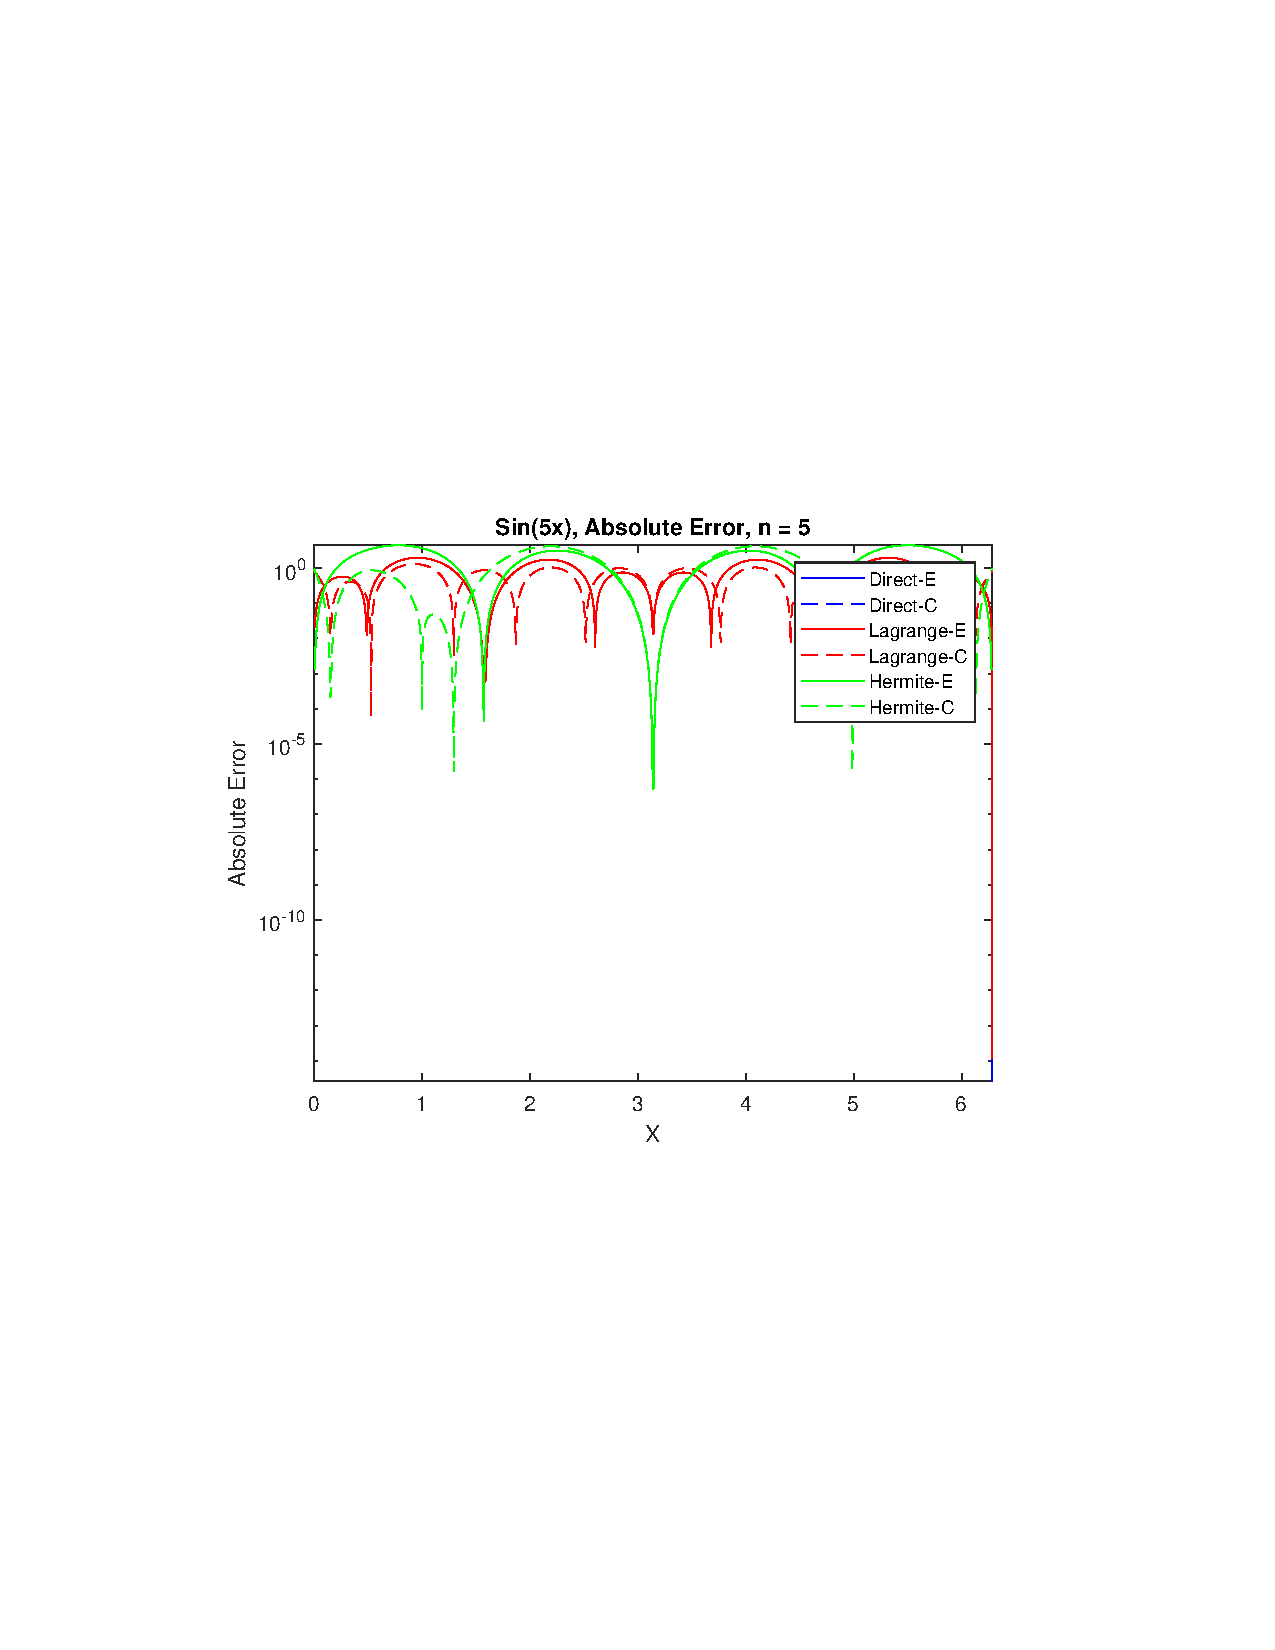
\includegraphics[width=9cm]{function2_absoluteError_5}\\
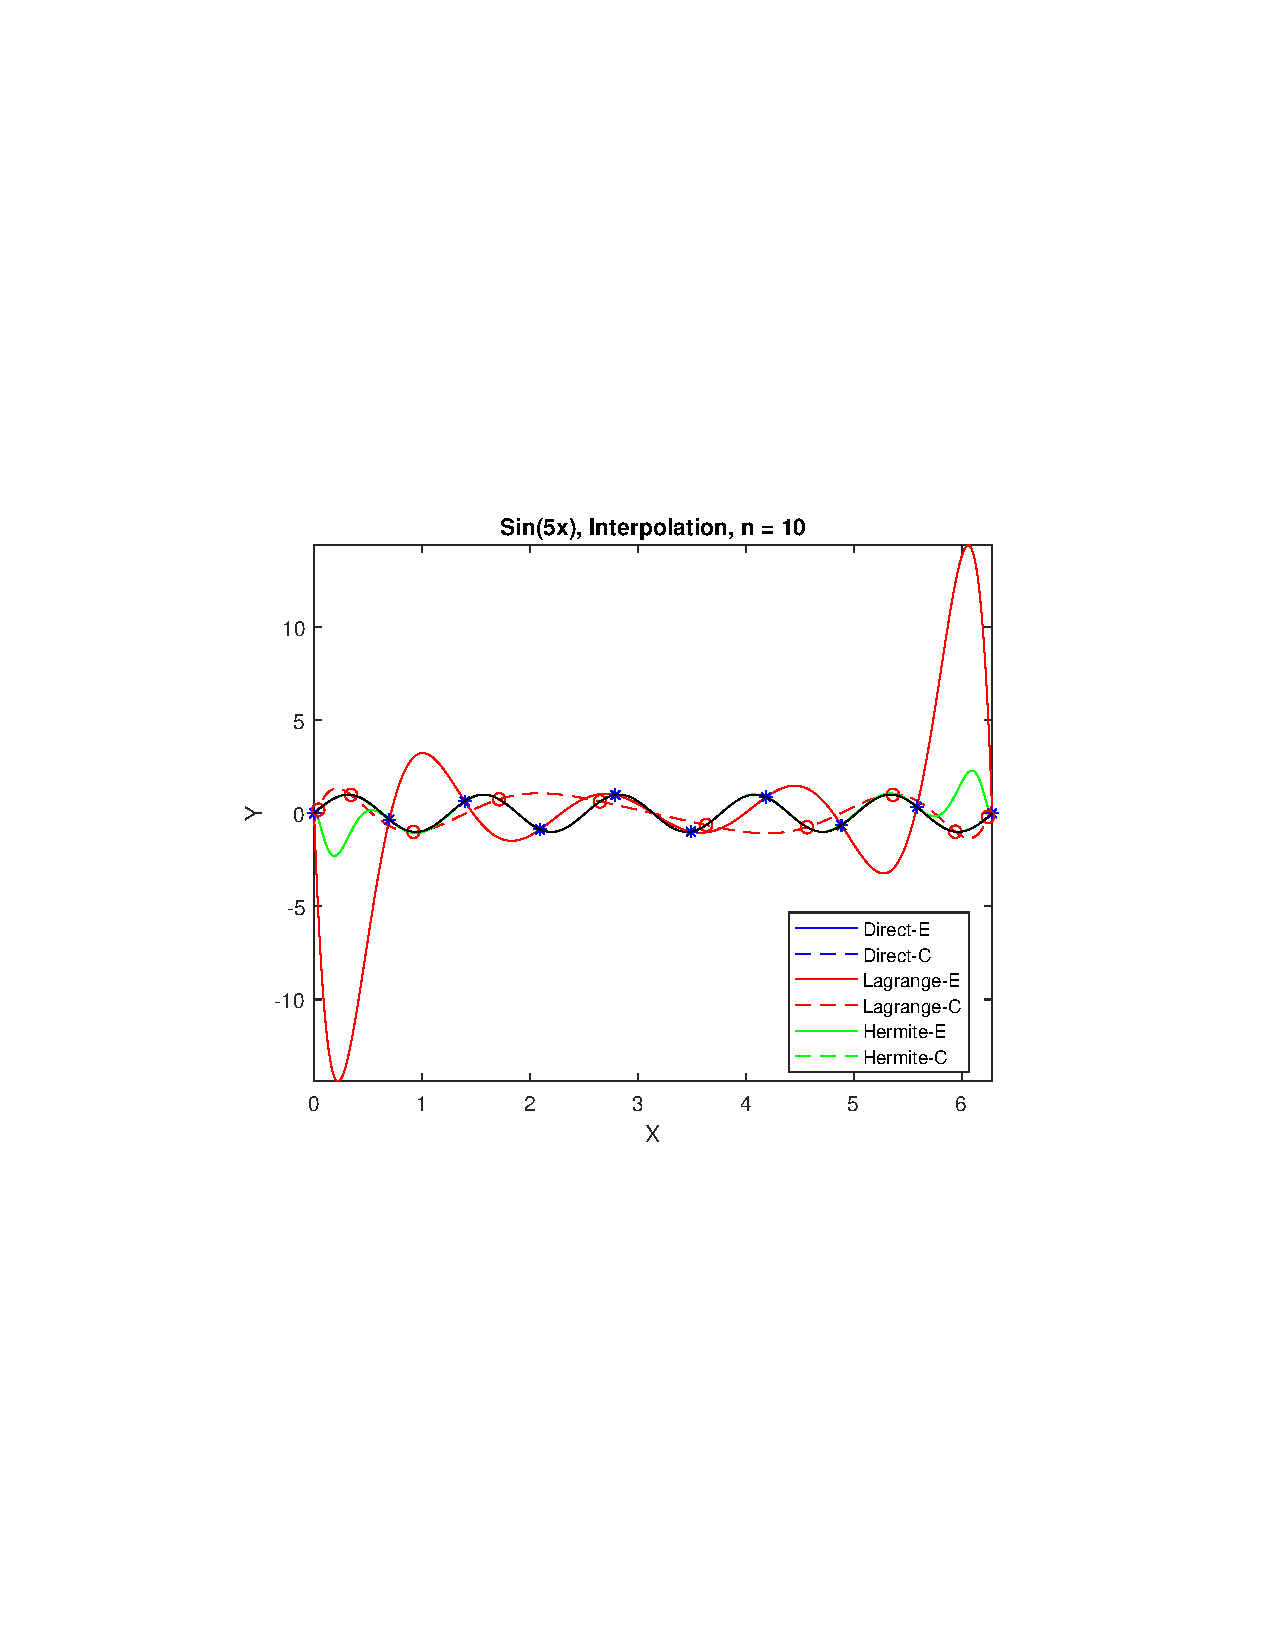
\includegraphics[width=9cm]{function2_10}%
\hskip -6em
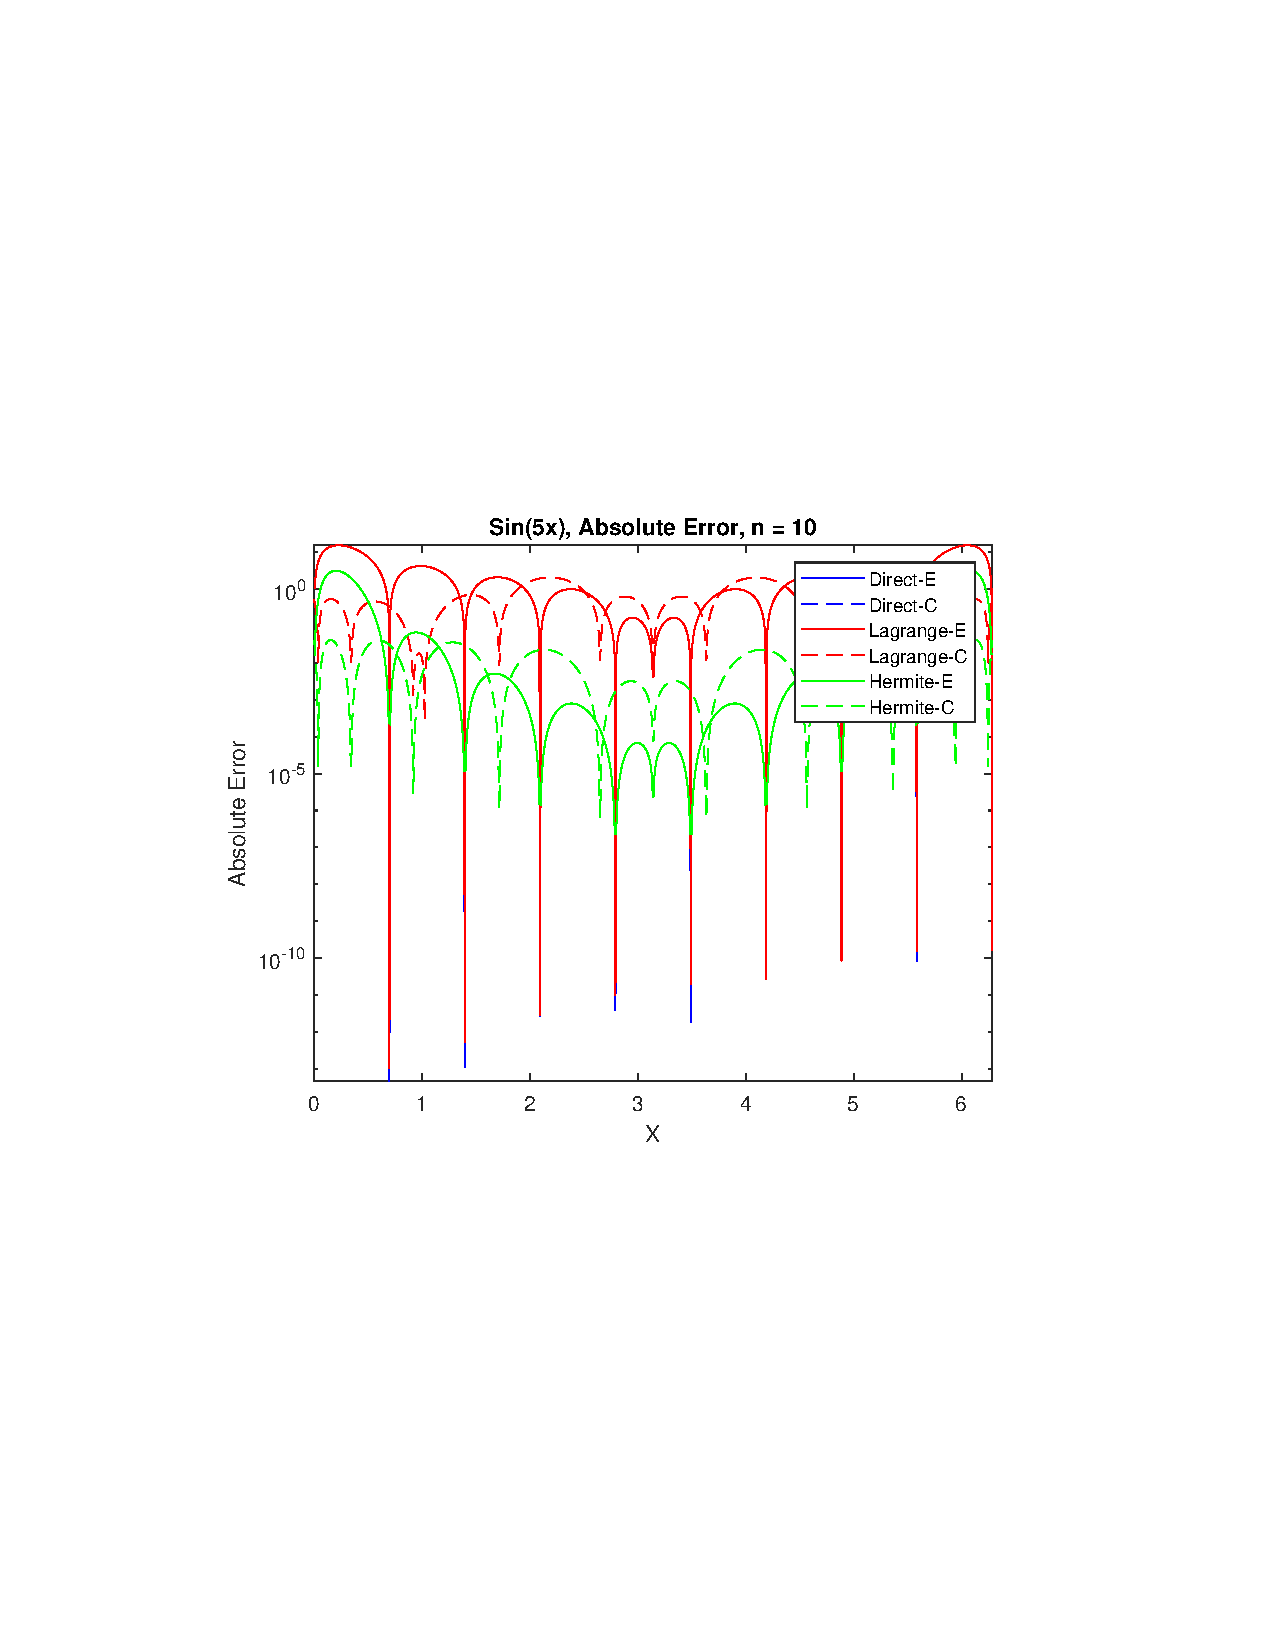
\includegraphics[width=9cm]{function2_absoluteError_10}\\
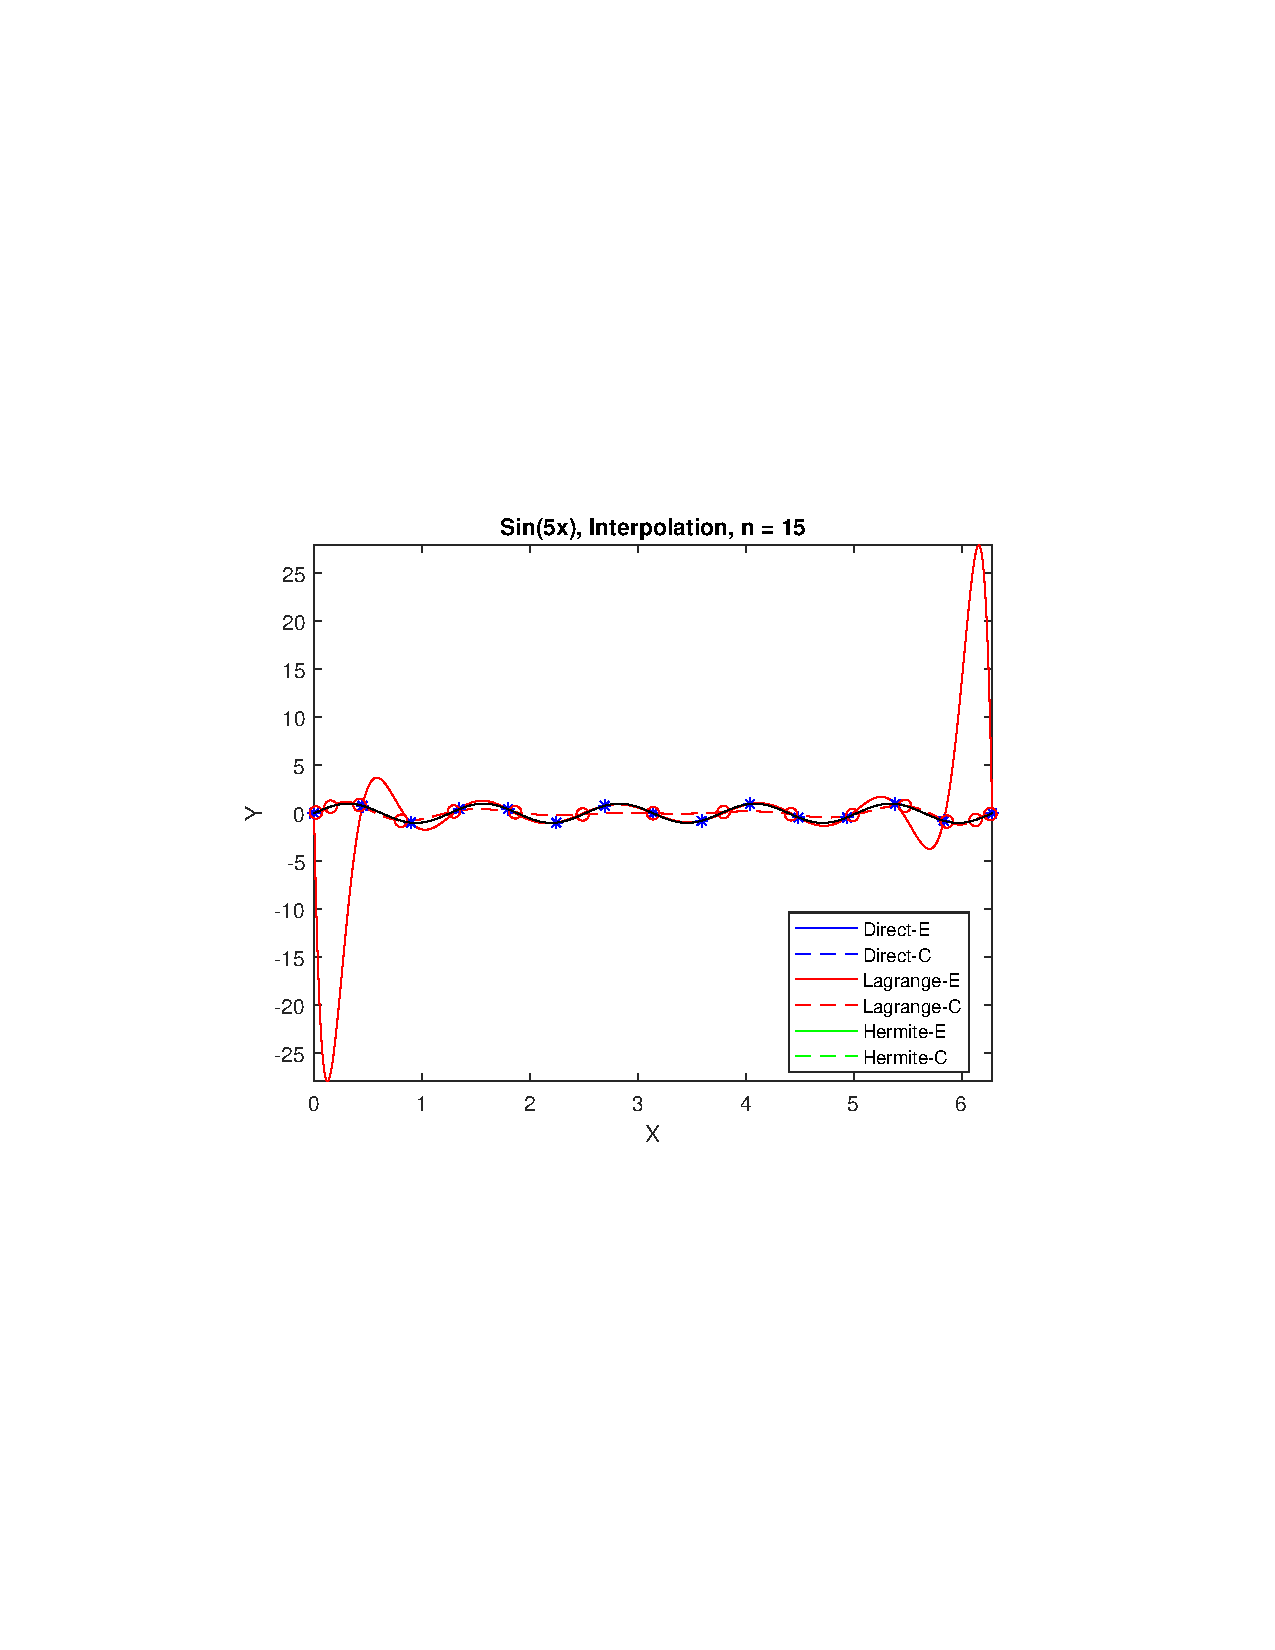
\includegraphics[width=9cm]{function2_15}%
\hskip -6em
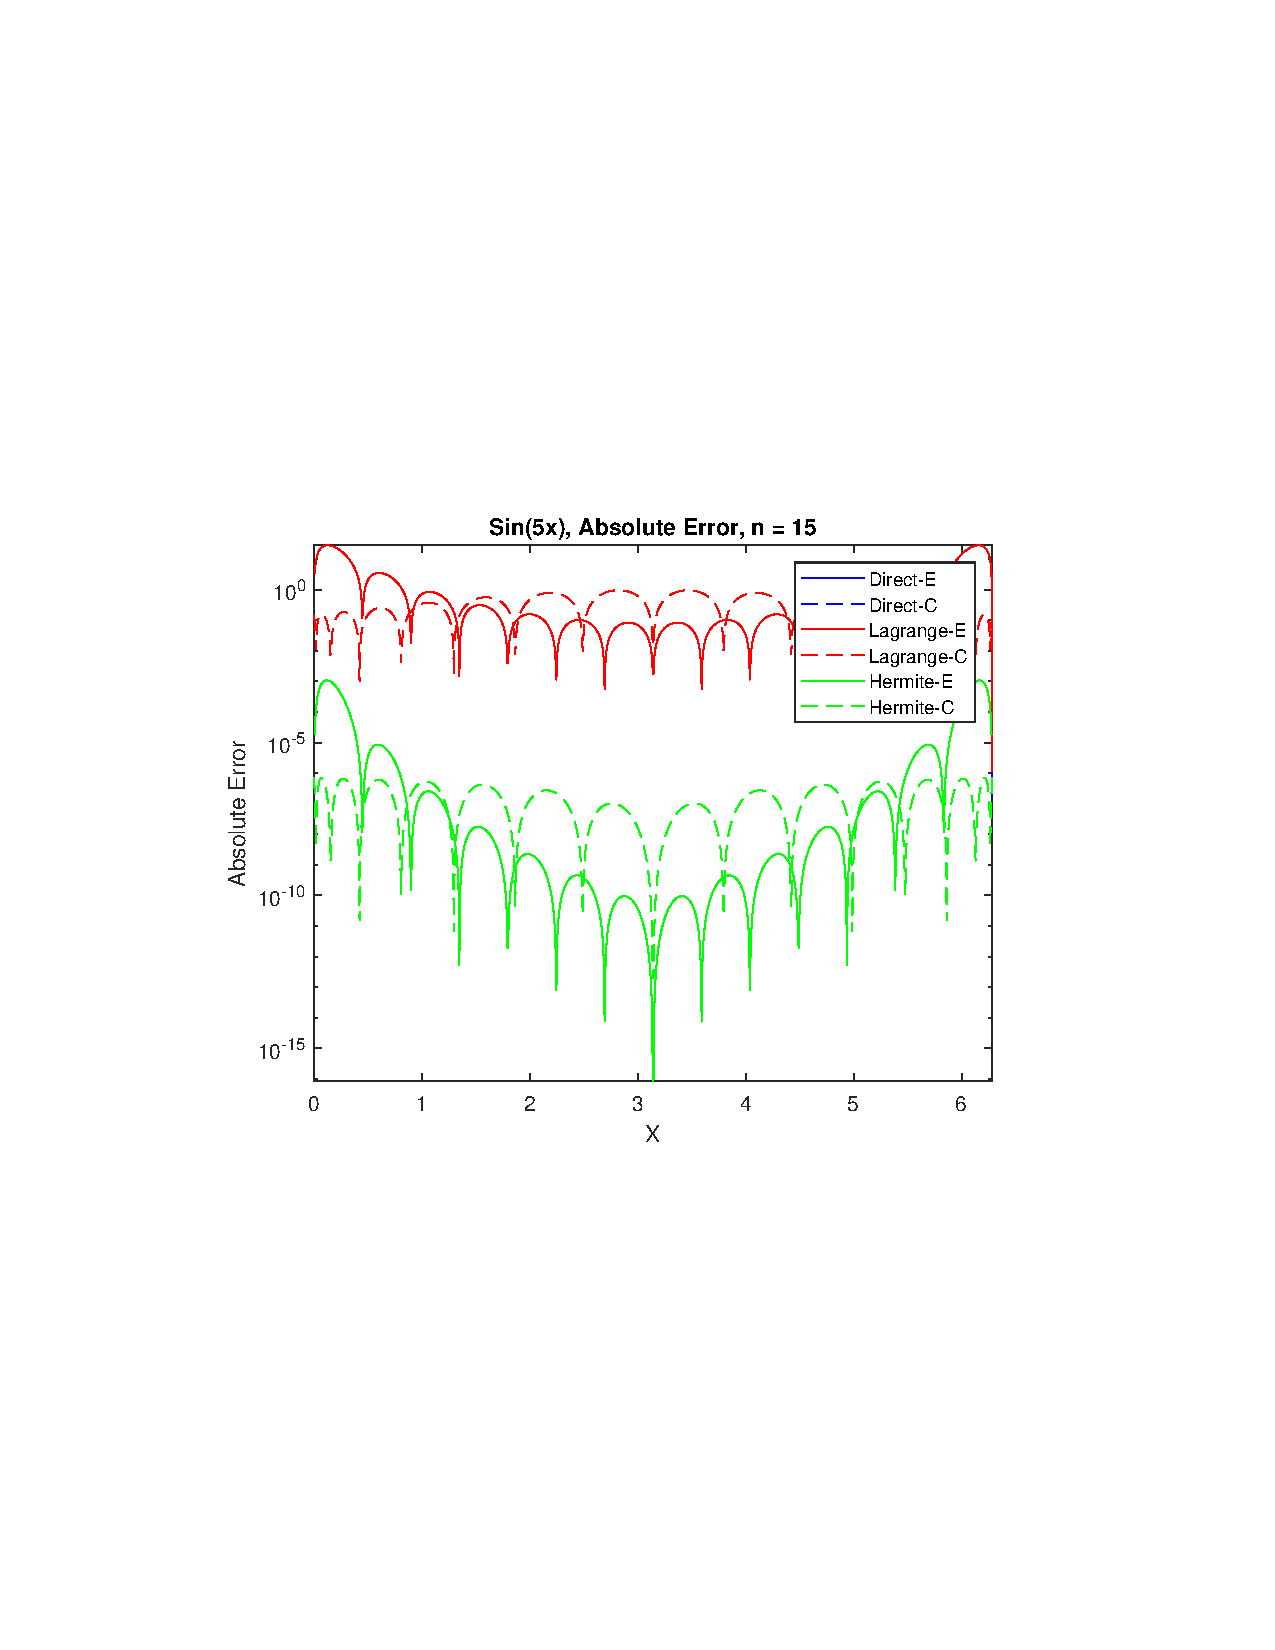
\includegraphics[width=9cm]{function2_absoluteError_15}\\
\end{figure}


\vspace{-100pt} % I can control the vertical spacing this way.
\begin{figure}[htp]
\setlength{\lineskip}{-170pt}
%\centering
\vspace{-170pt} % I can control the vertical spacing this way.
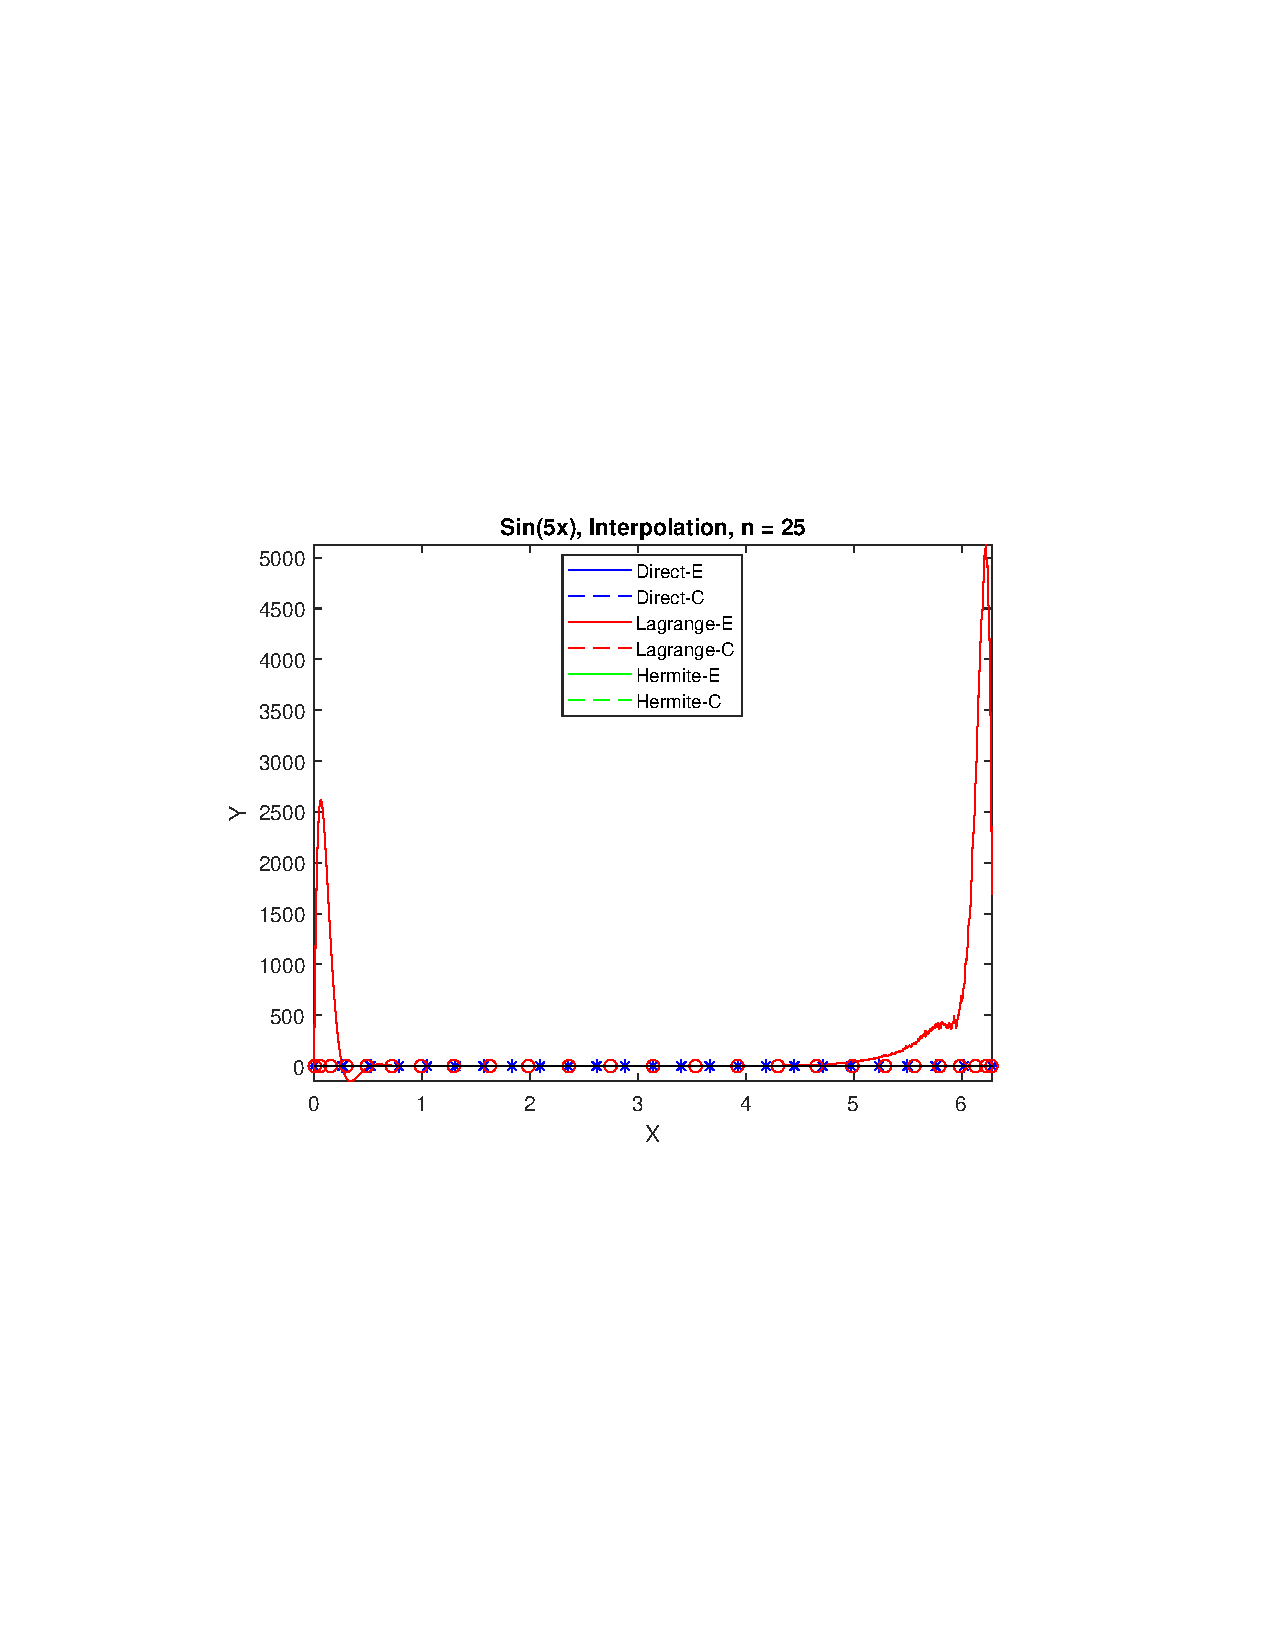
\includegraphics[width=8cm]{function2_25}%
\hskip -3em
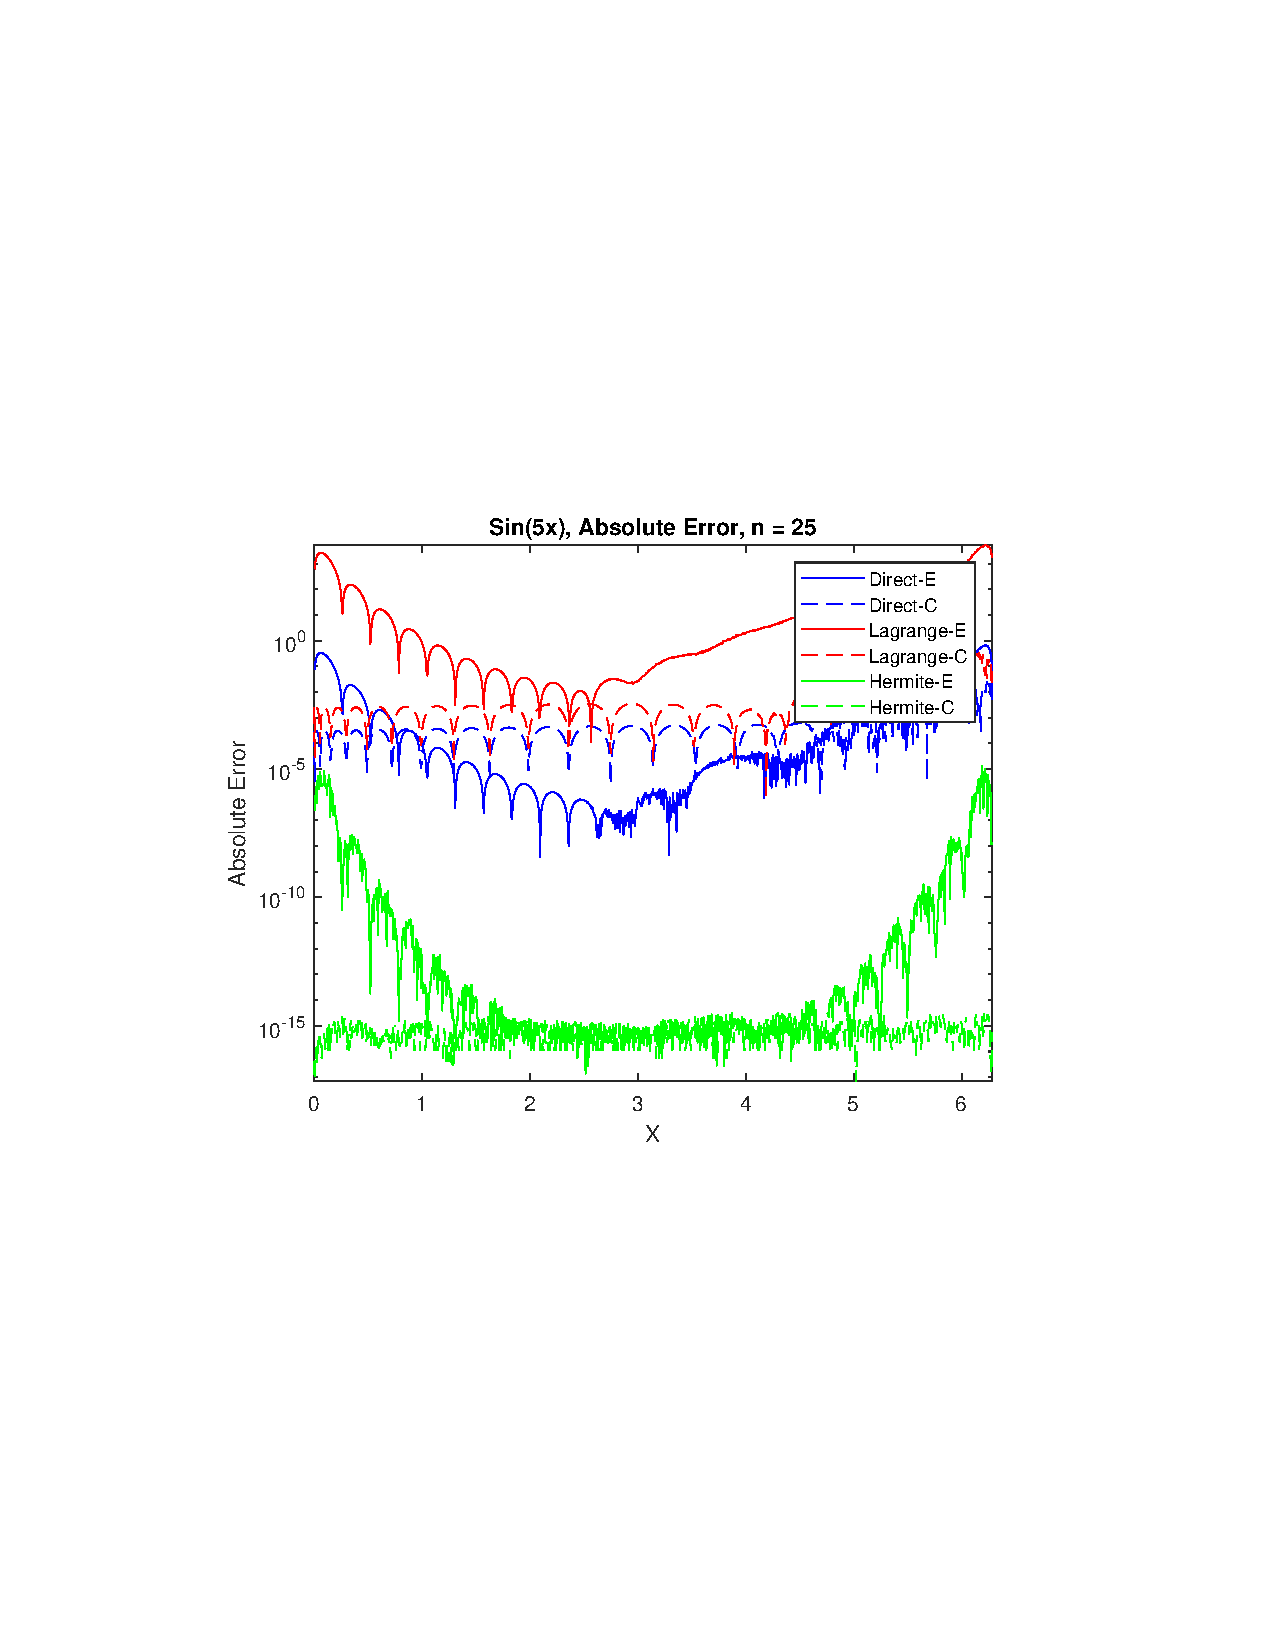
\includegraphics[width=8cm]{function2_absoluteError_25}\\
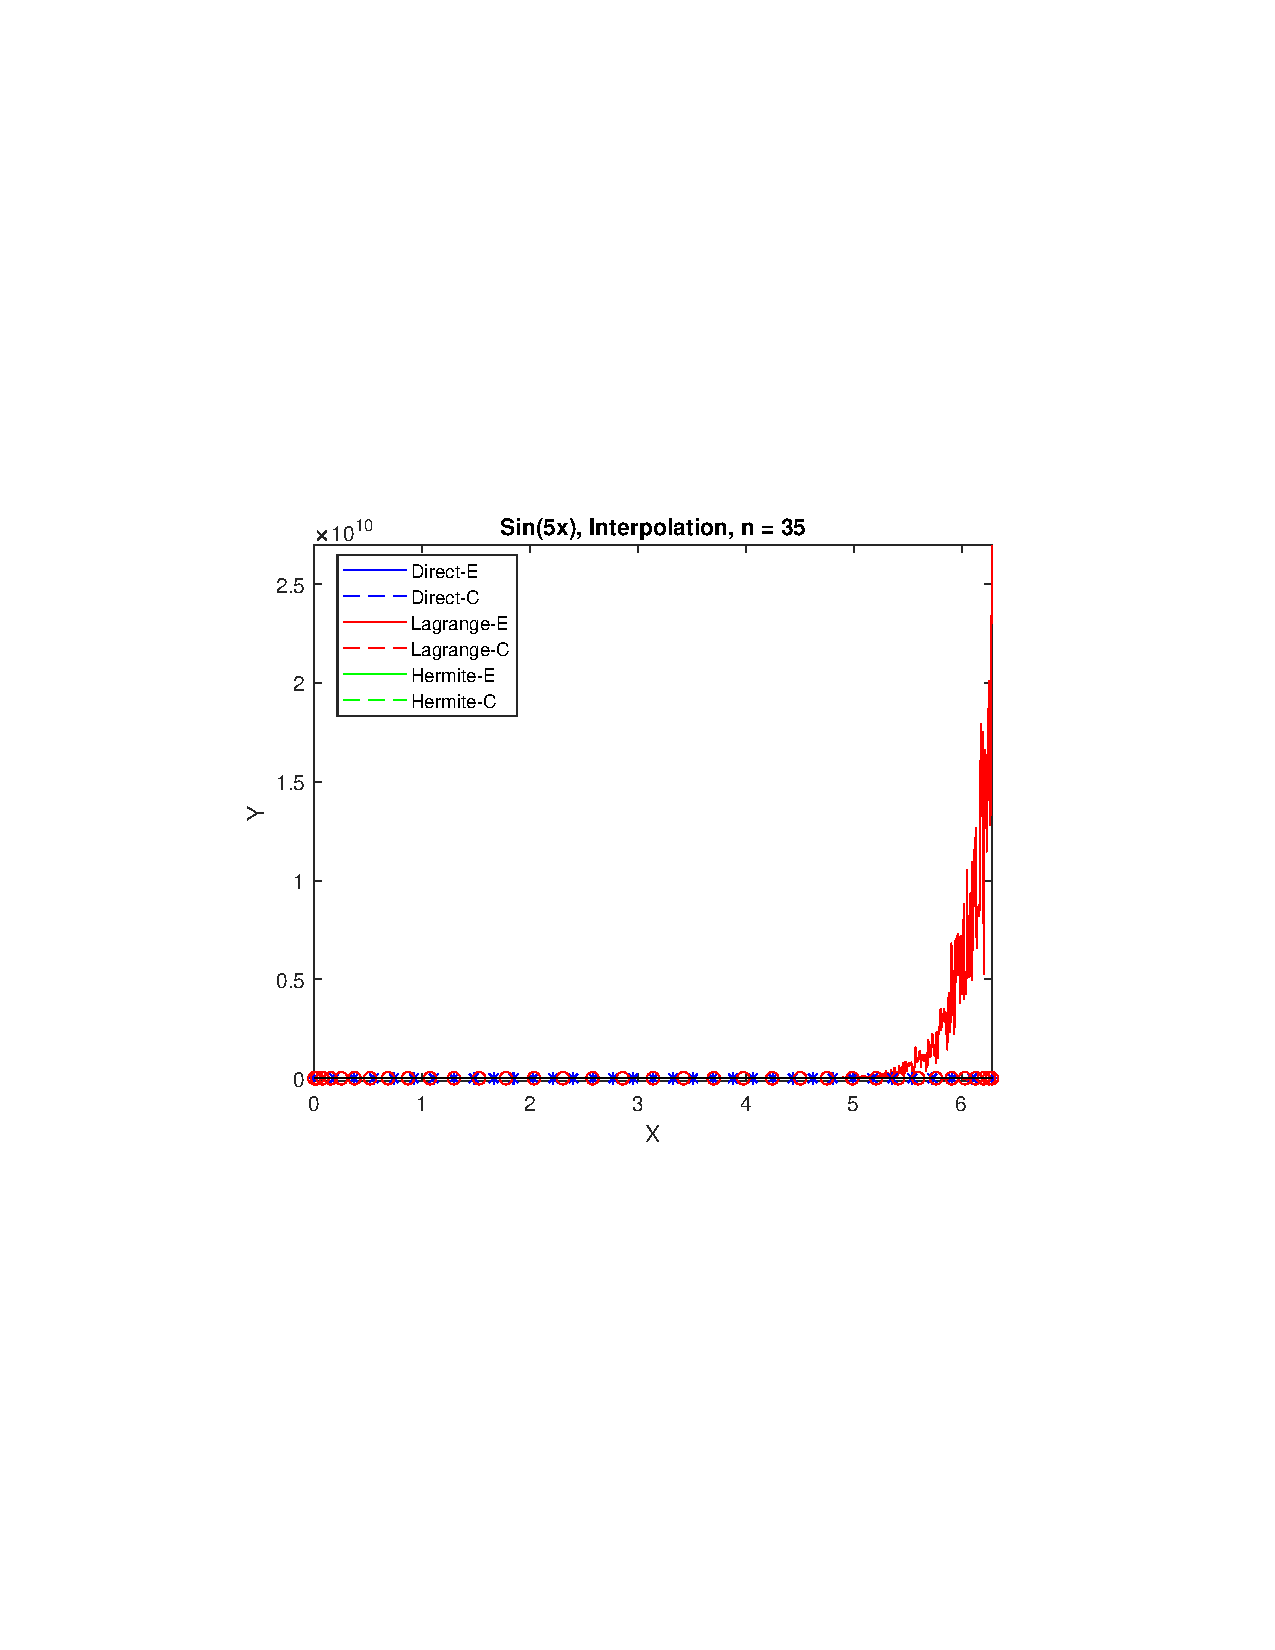
\includegraphics[width=8cm]{function2_35}
\hskip -3em%
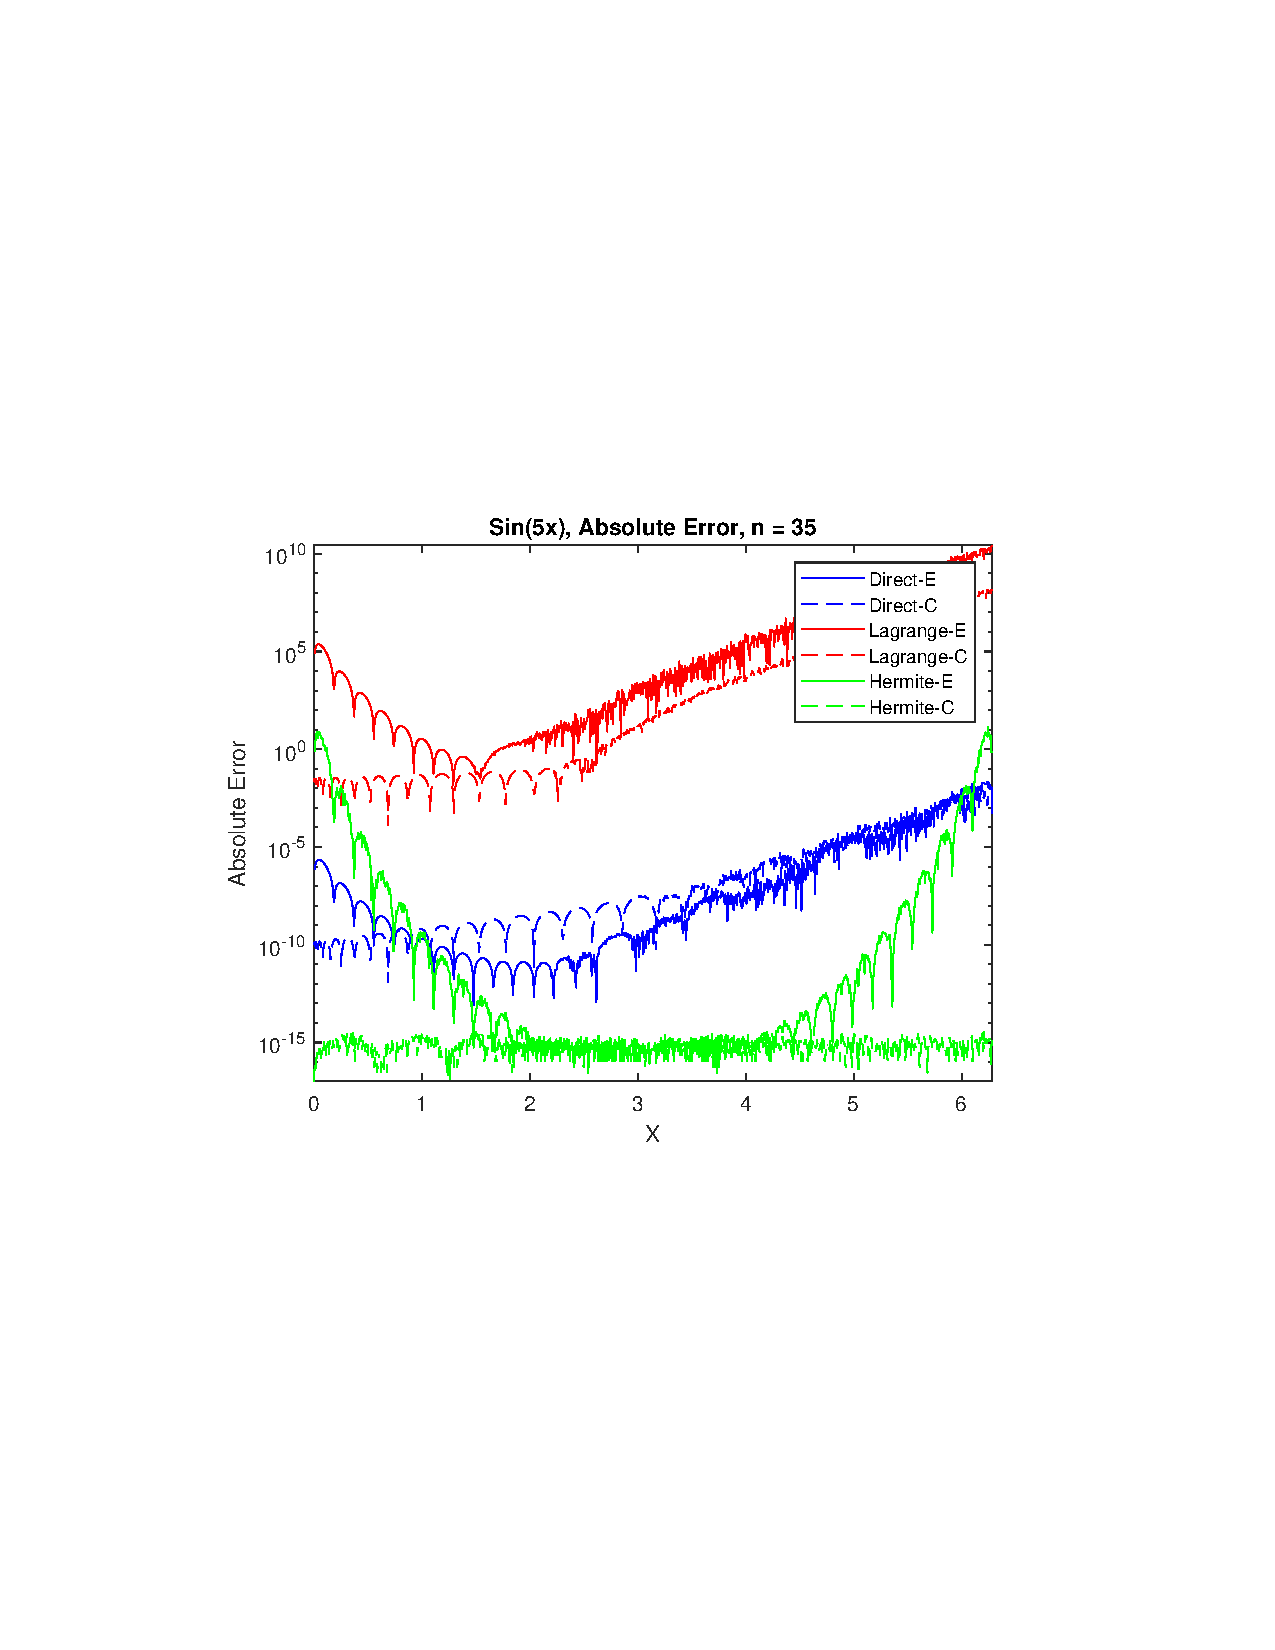
\includegraphics[width=8cm]{function2_absoluteError_35}\\

\vspace{-100pt} % I can control the vertical spacing this way.
\caption{Approximation \& error analysis of $Sin(5x)$.}
\end{figure}
%


\clearpage
\newpage
\subsection{$f\left(x\right) =\dfrac{1}{1+x^2}$}
% Breaking Sin(5x) Figures up into sub figures: 3 rows of 2 & 2 rows of 2.
\vspace{25pt}
\begin{figure}[htp]
\setlength{\lineskip}{-205pt}
\centering
\vspace{-125pt} % I can control the vertical spacing this way.
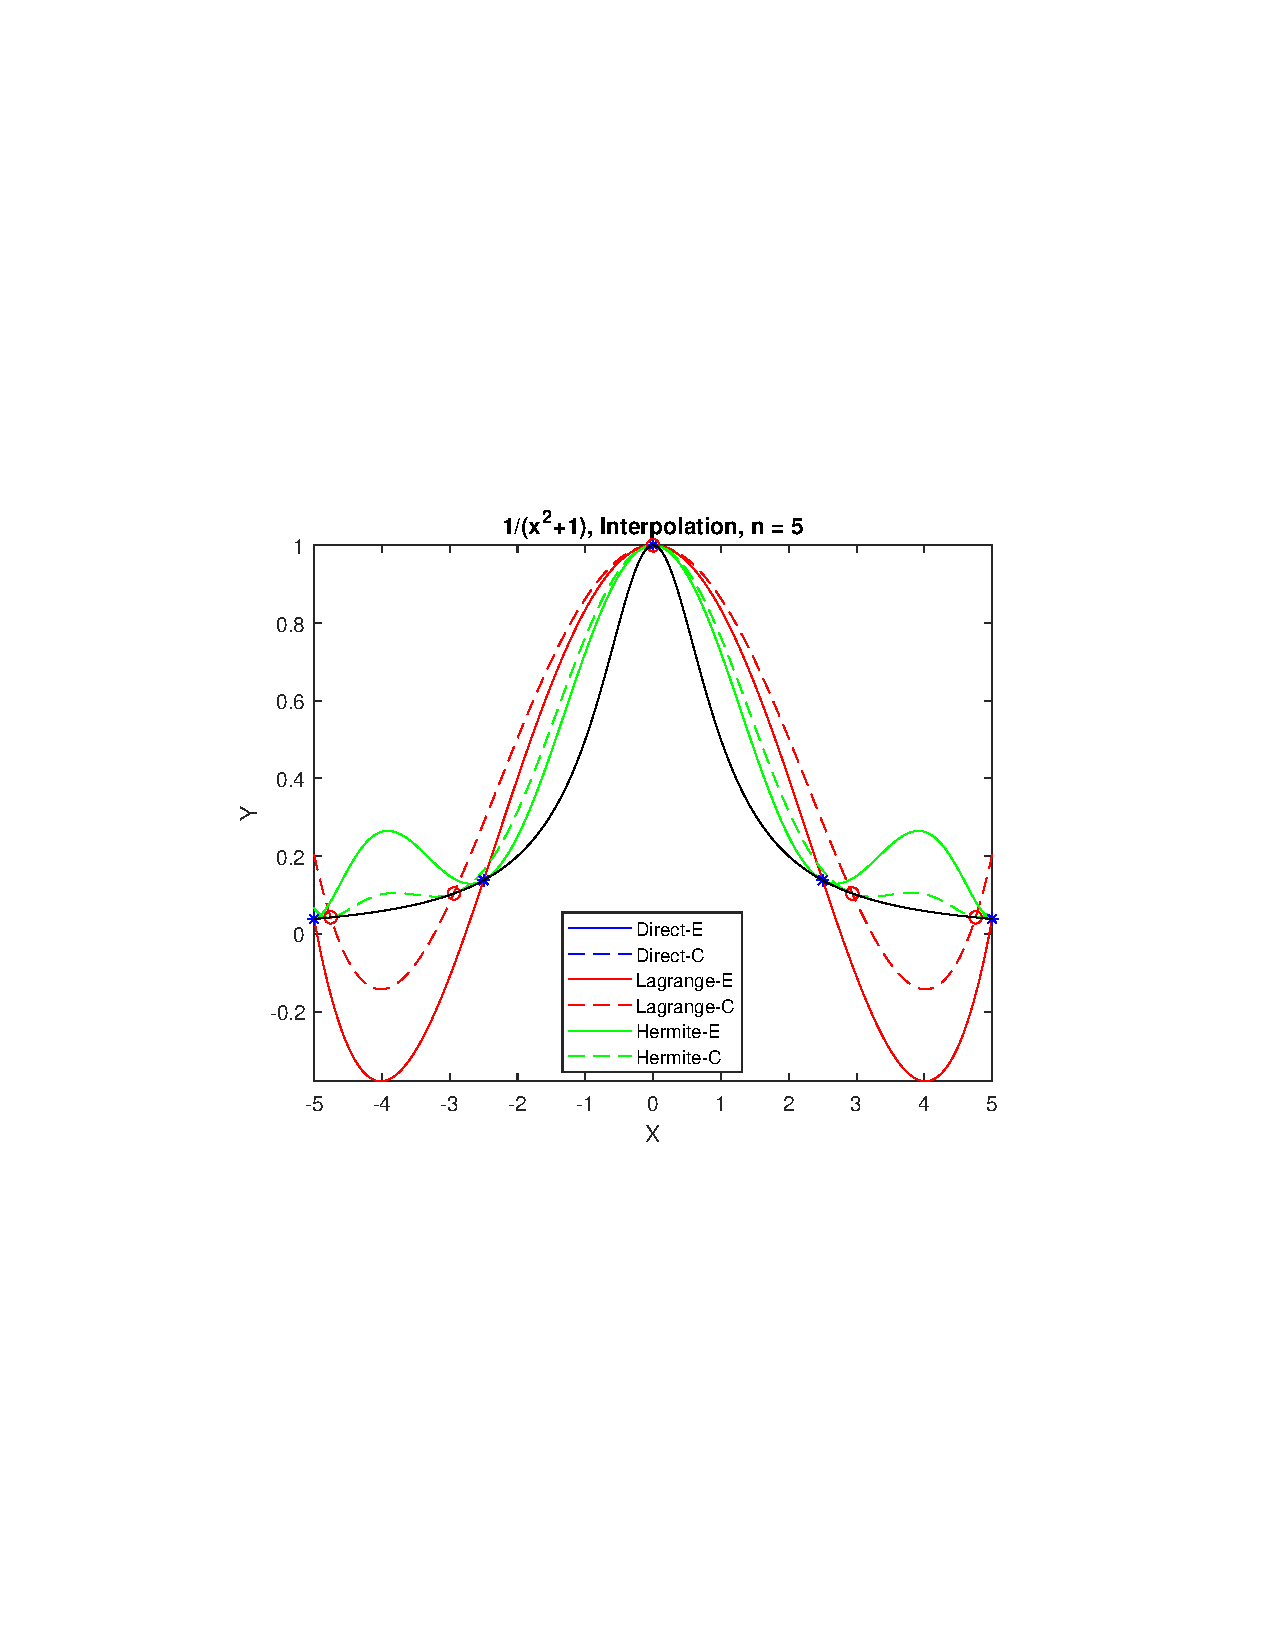
\includegraphics[width=9cm]{function3_5}%
\hskip -6em
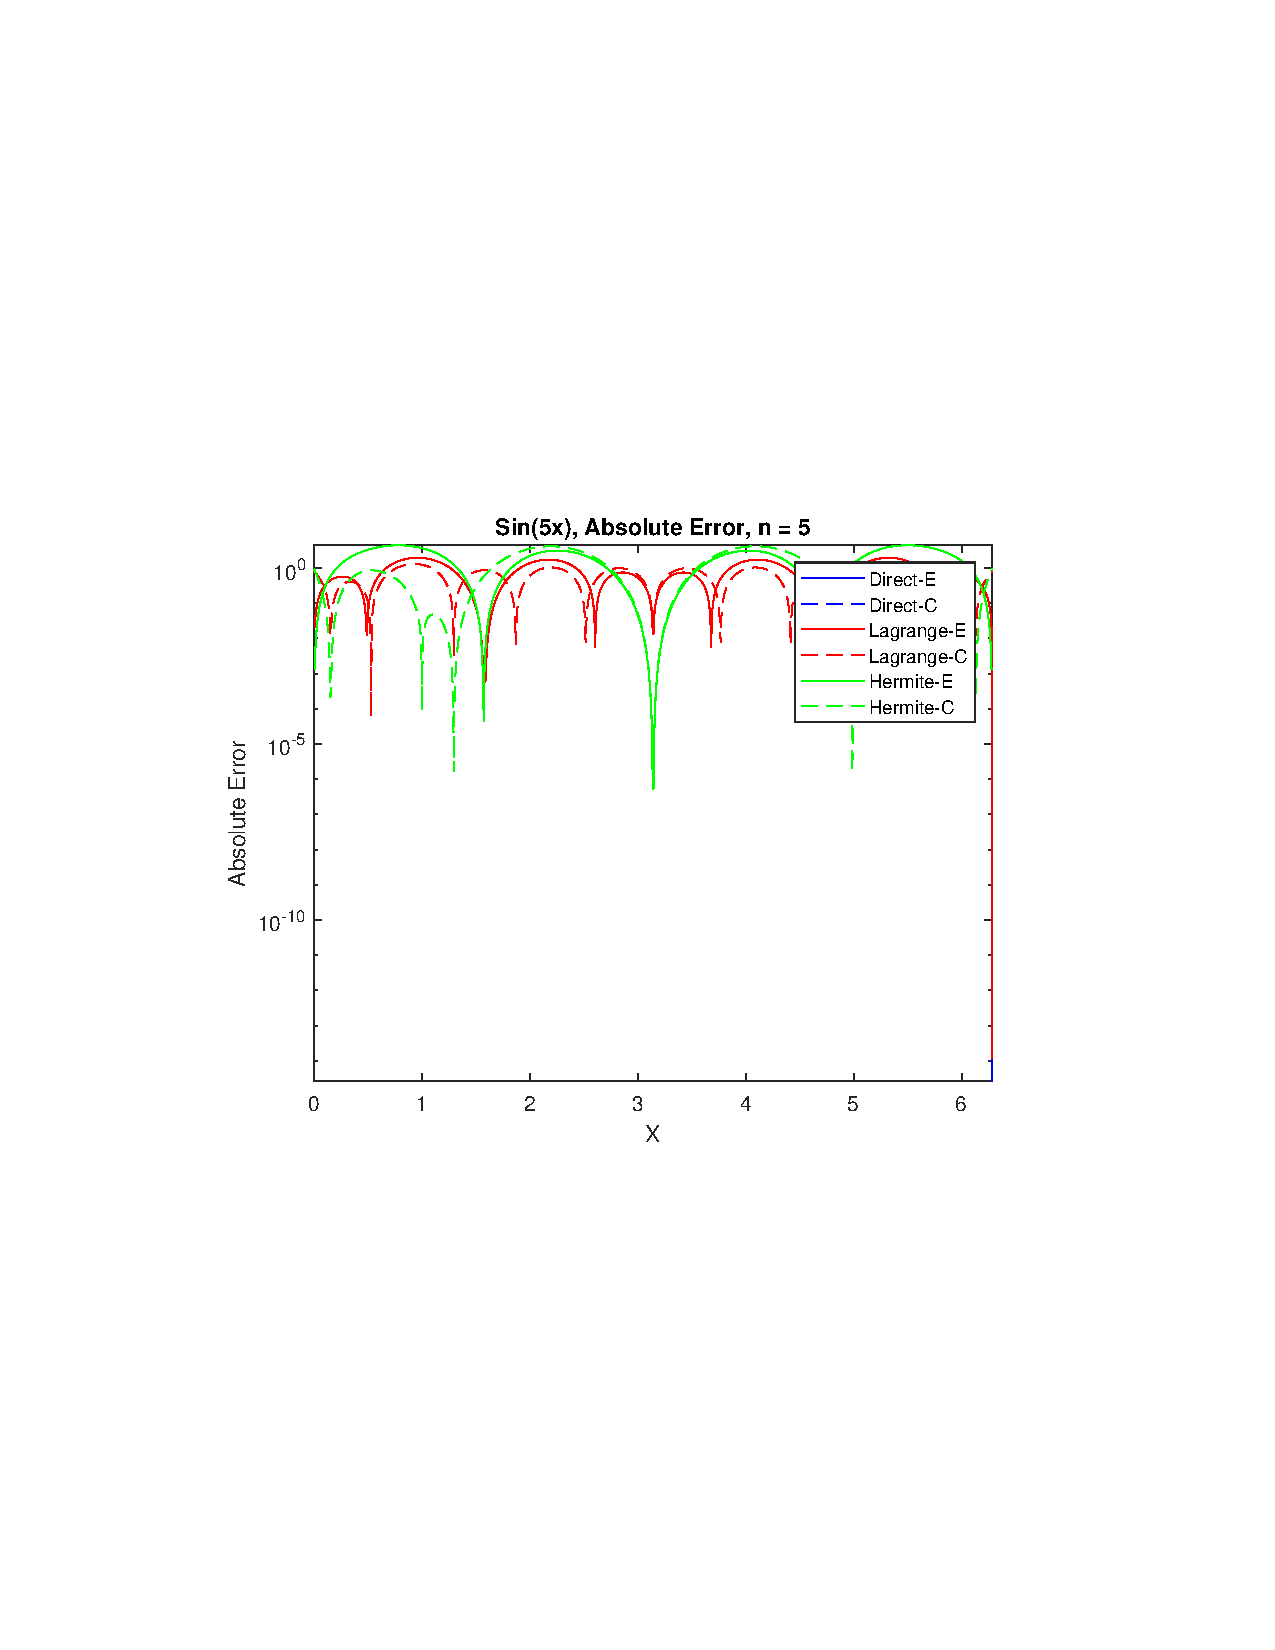
\includegraphics[width=9cm]{function2_absoluteError_5}\\
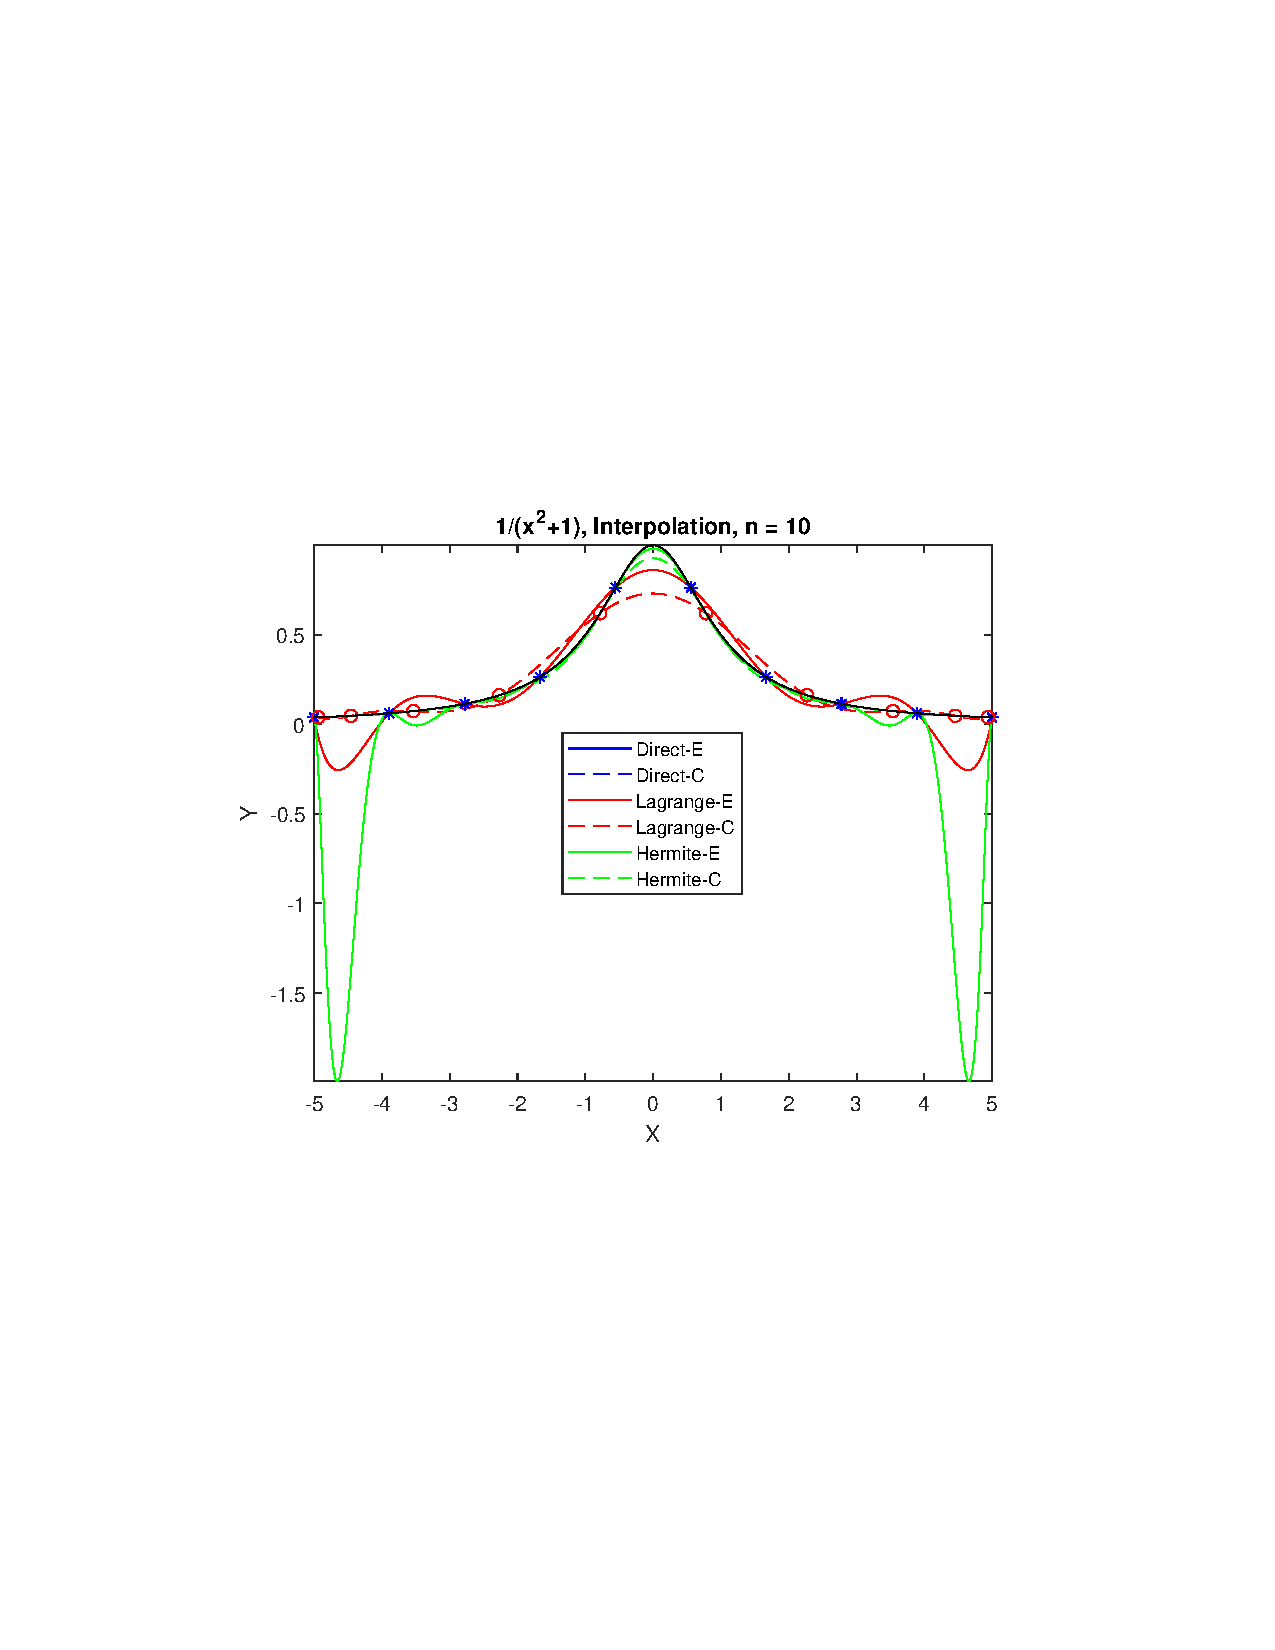
\includegraphics[width=9cm]{function3_10}%
\hskip -6em
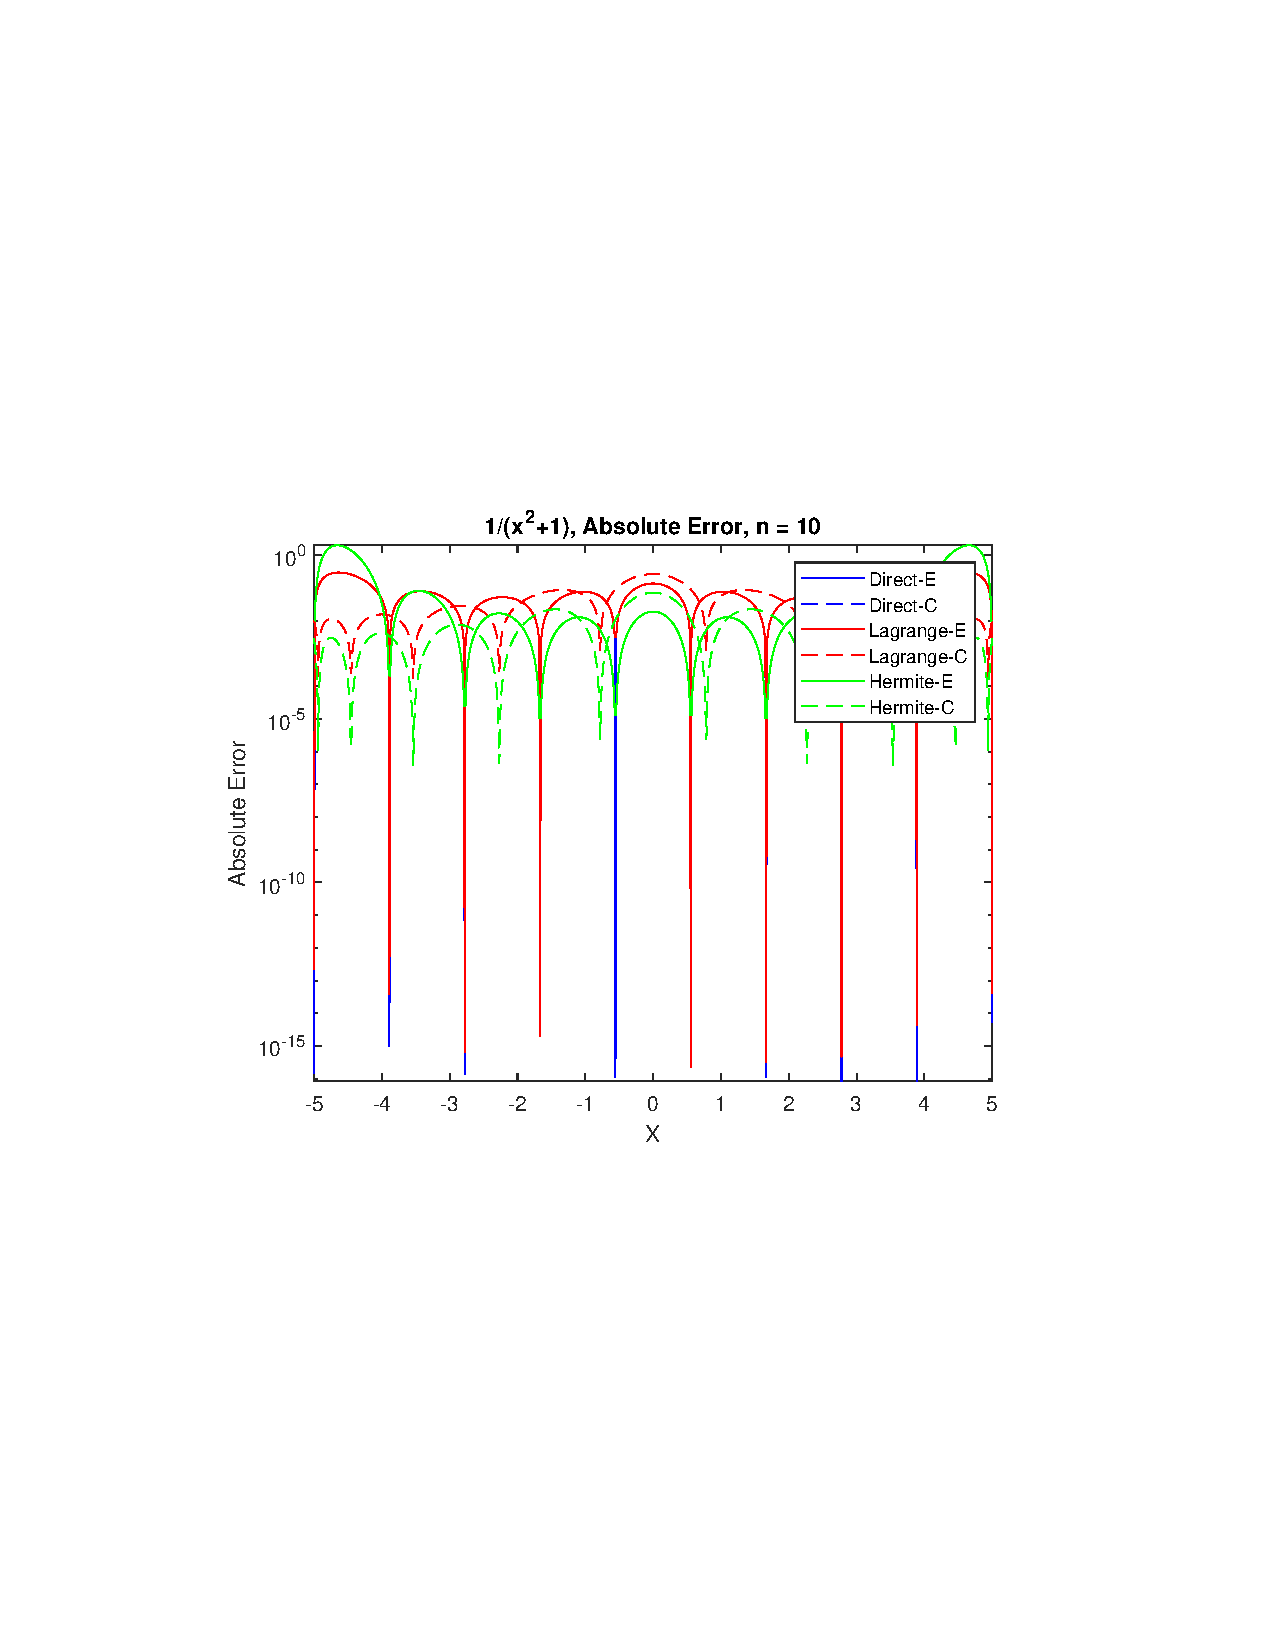
\includegraphics[width=9cm]{function3_absoluteError_10}\\
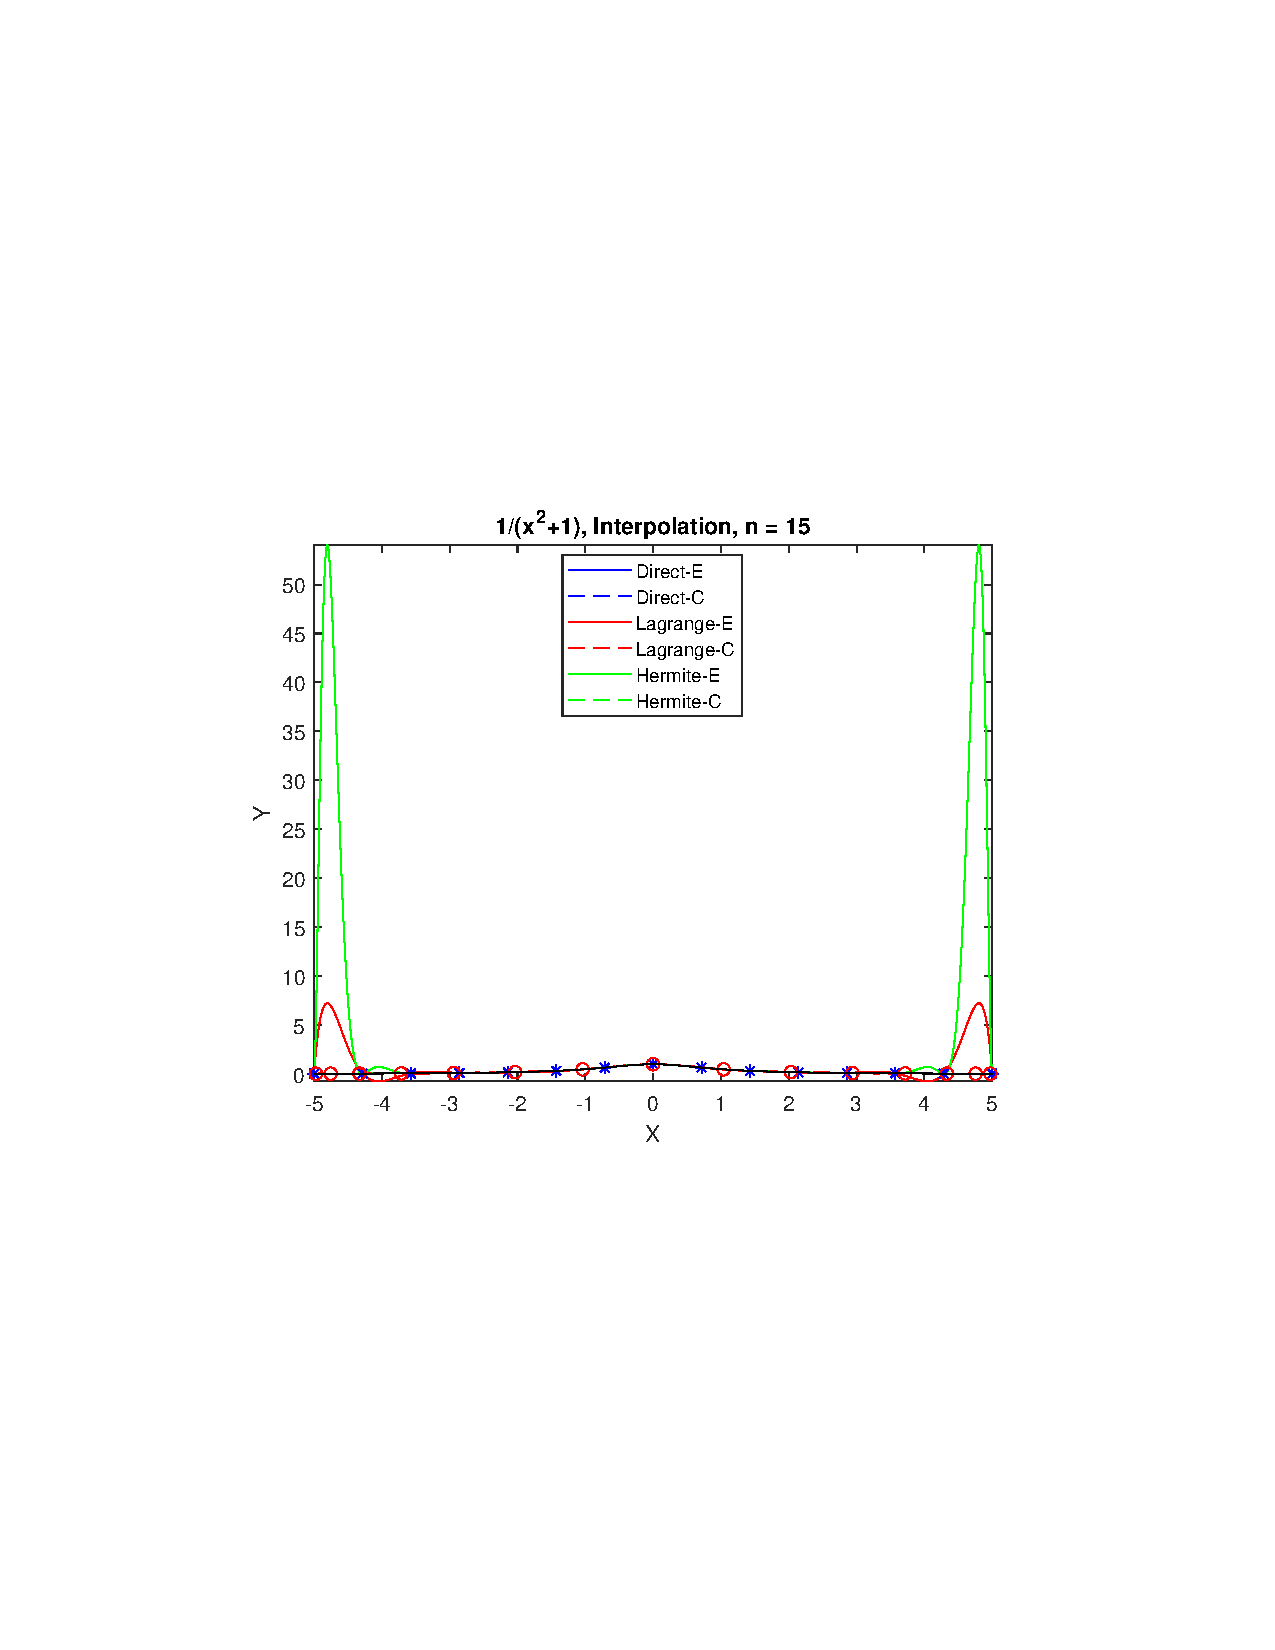
\includegraphics[width=9cm]{function3_15}%
\hskip -6em
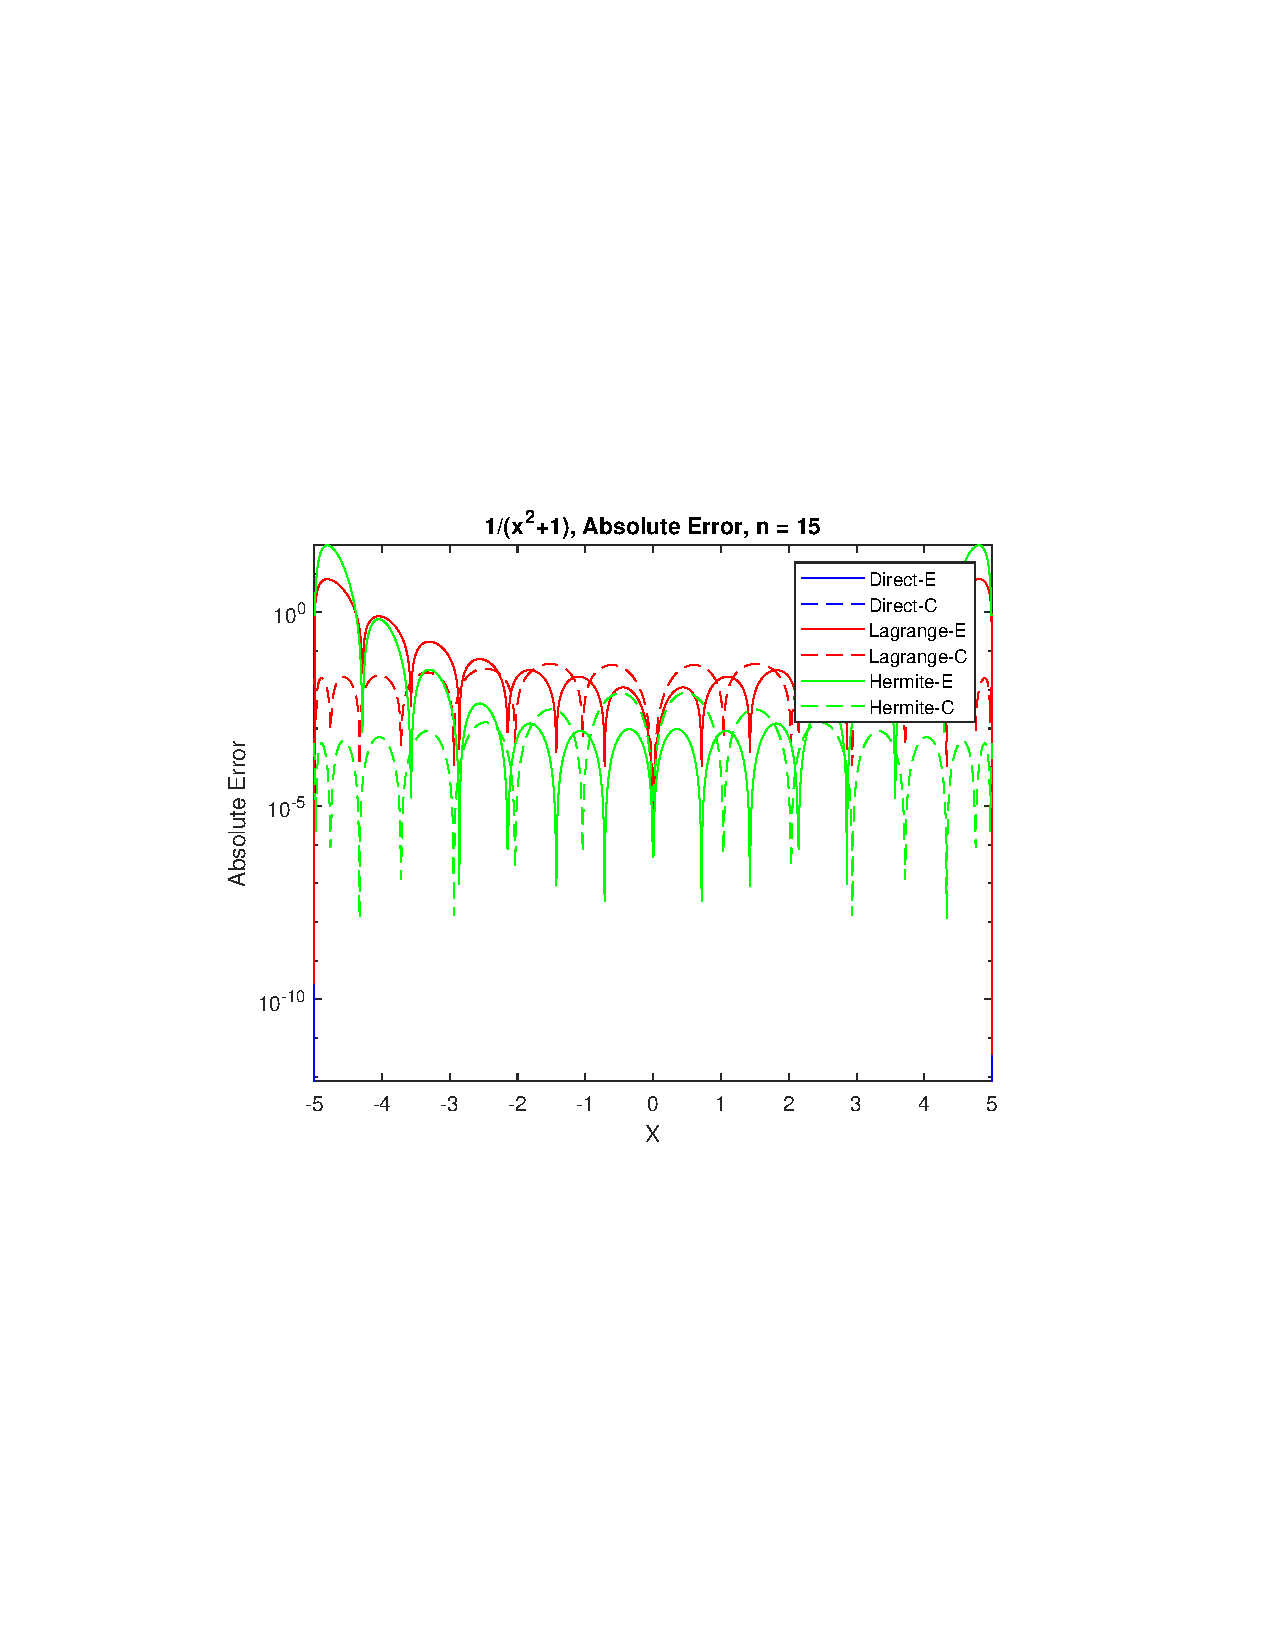
\includegraphics[width=9cm]{function3_absoluteError_15}\\
\end{figure}


\vspace{-100pt} % I can control the vertical spacing this way.
\begin{figure}[htp]
\setlength{\lineskip}{-170pt}
%\centering
\vspace{-170pt} % I can control the vertical spacing this way.
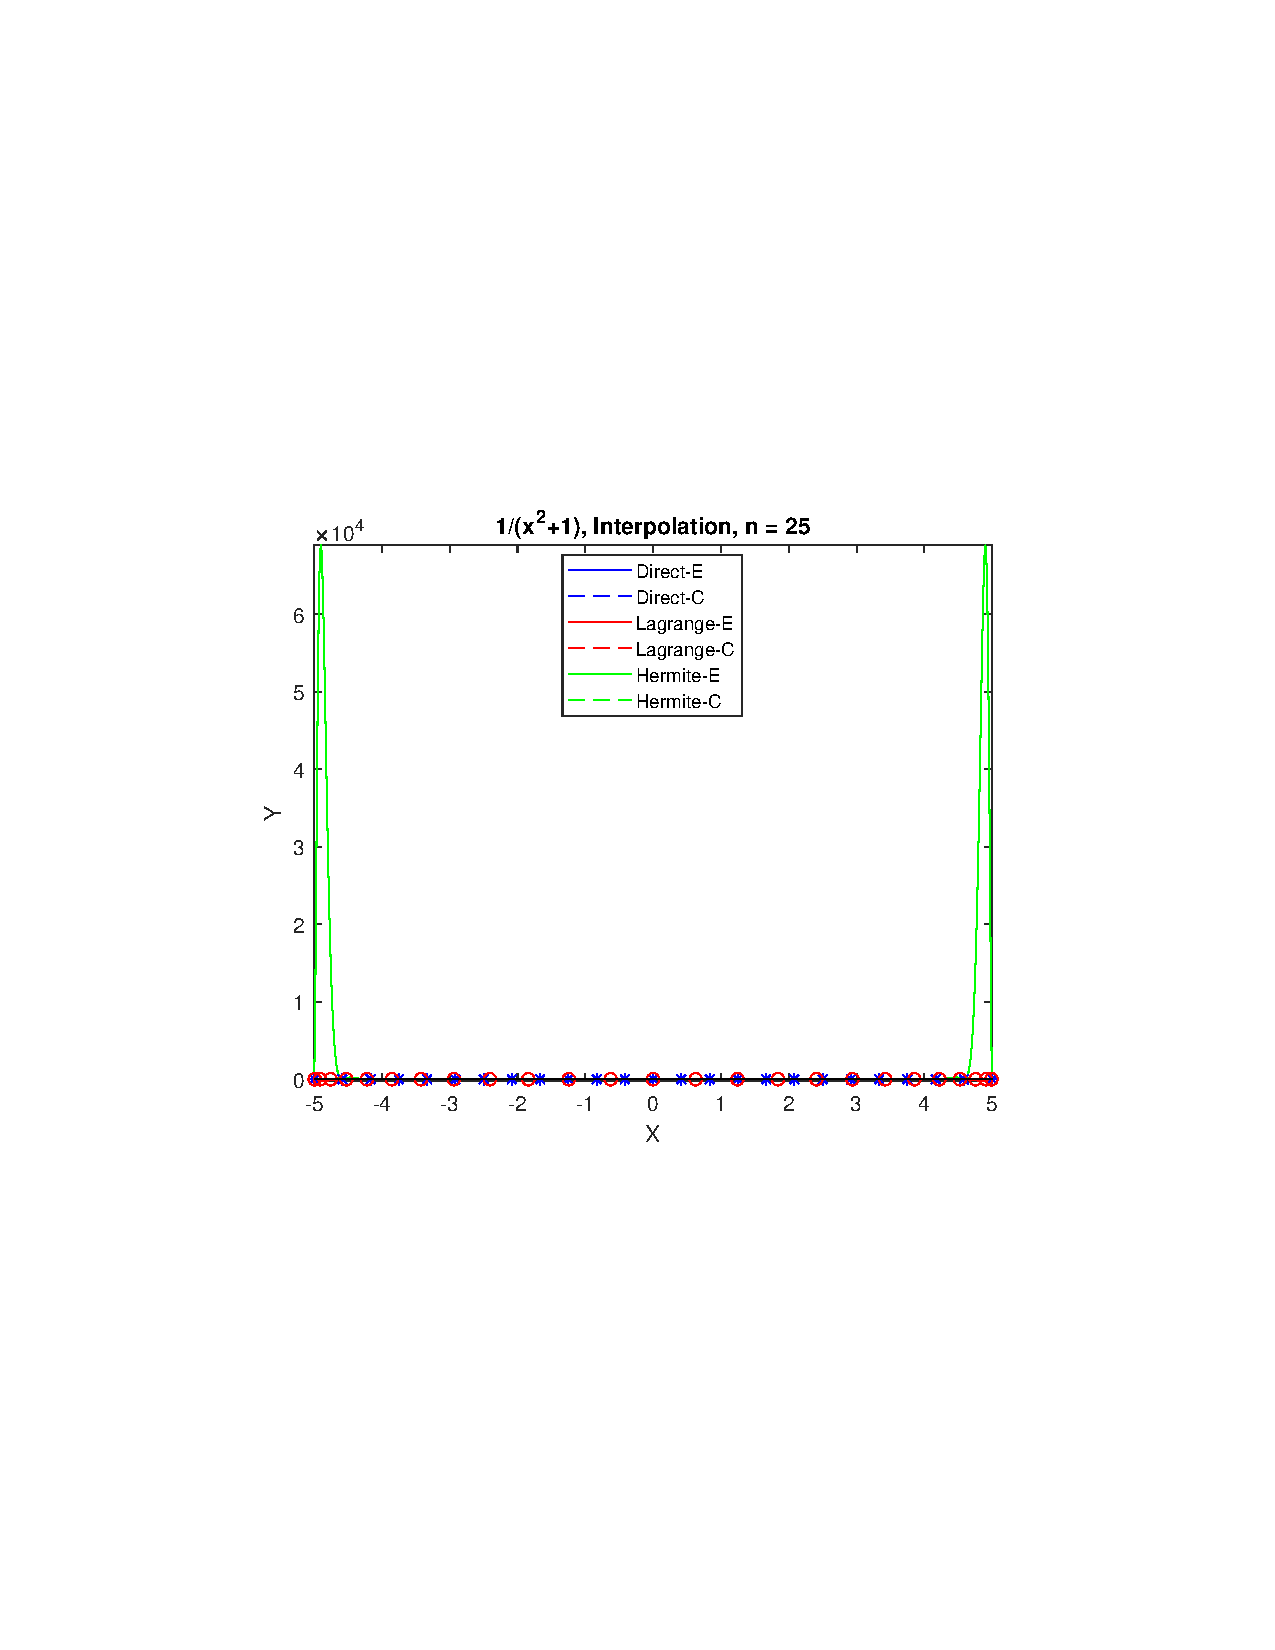
\includegraphics[width=8cm]{function3_25}%
\hskip -3em
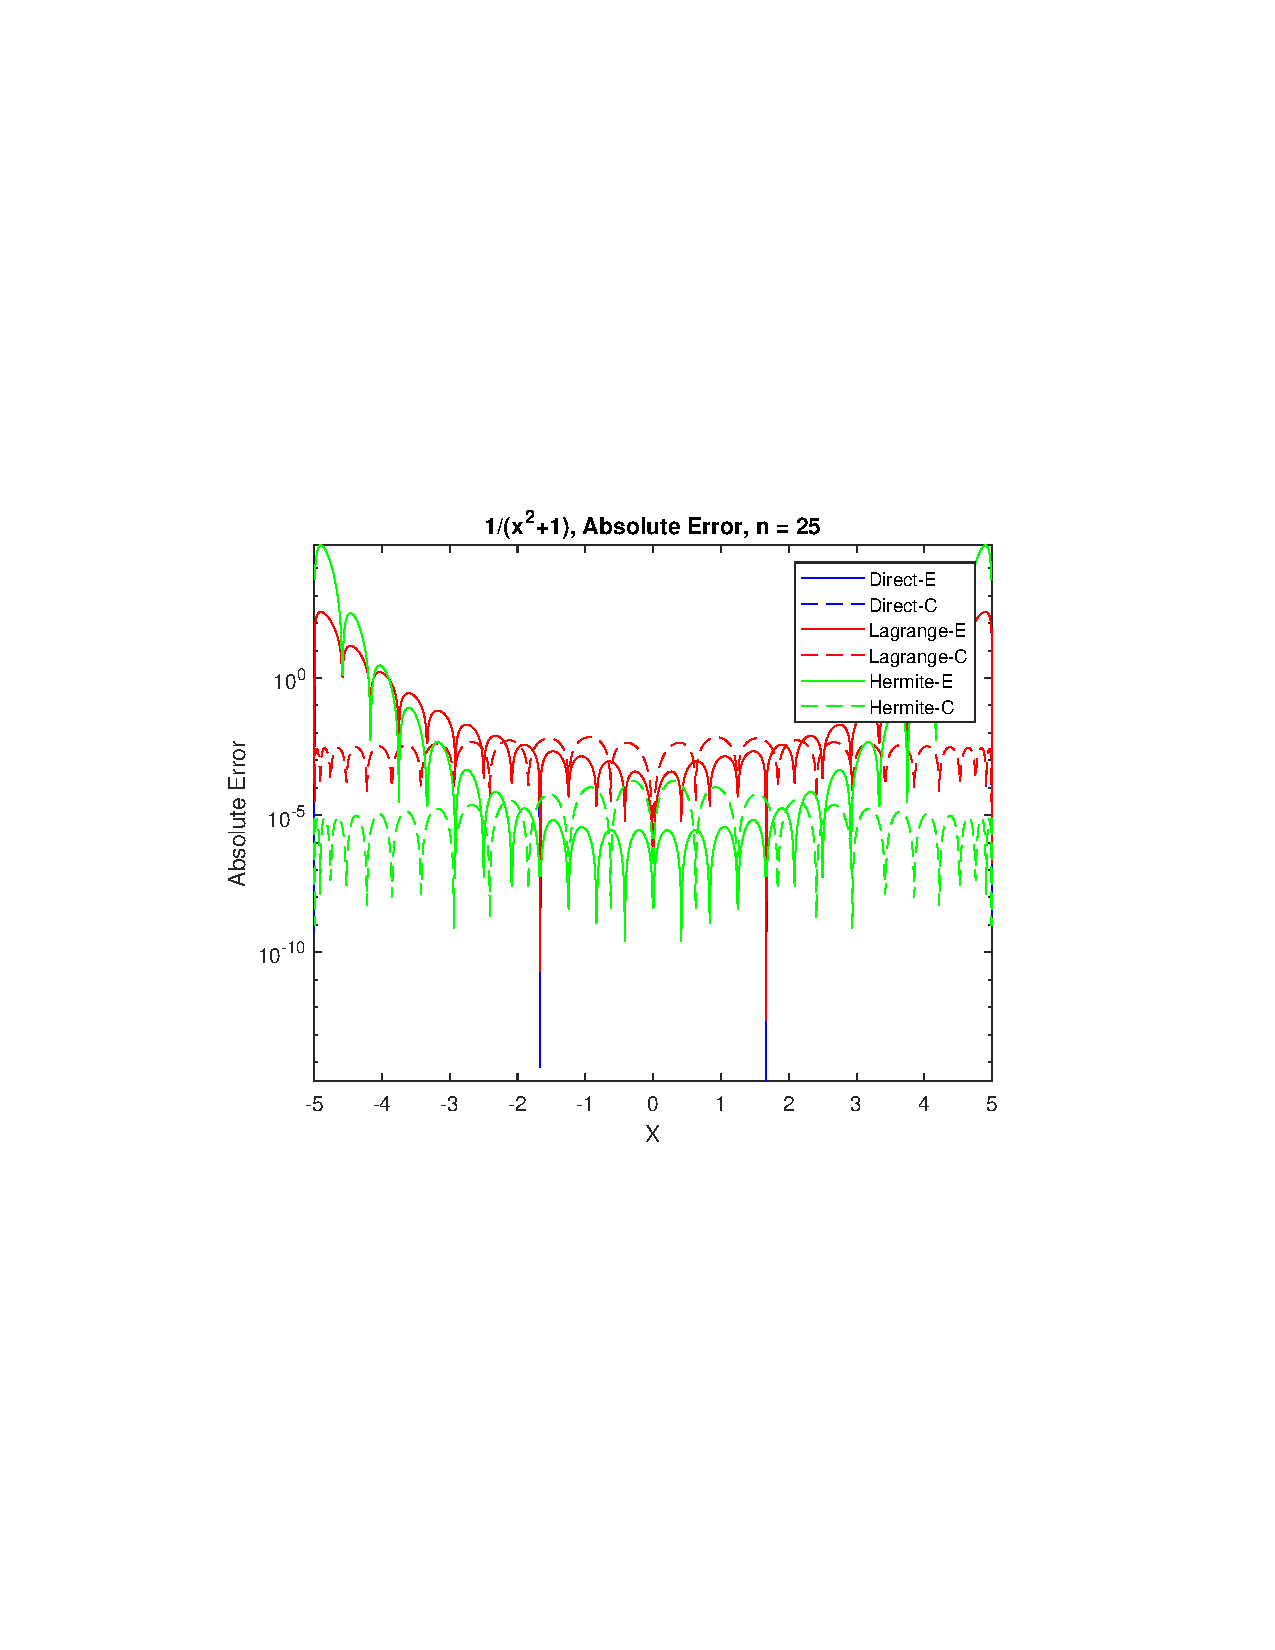
\includegraphics[width=8cm]{function3_absoluteError_25}\\
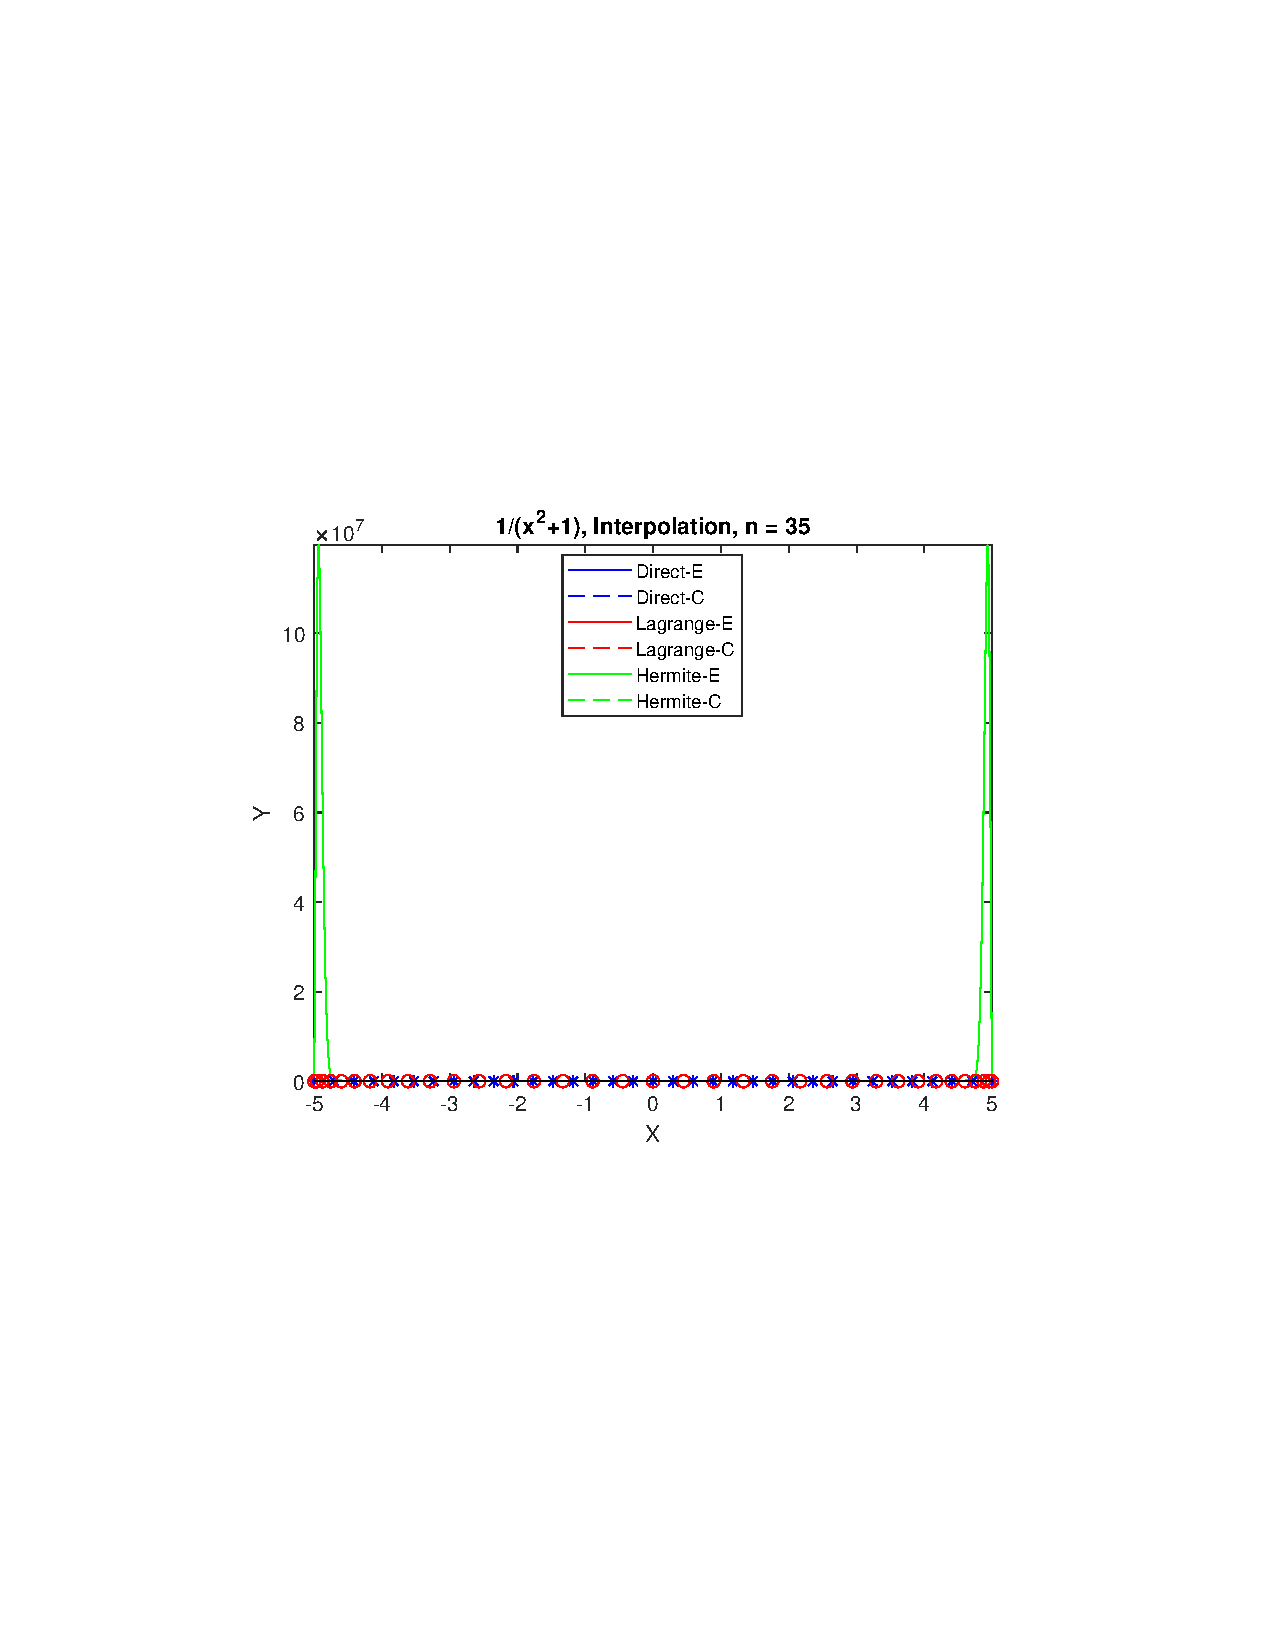
\includegraphics[width=8cm]{function3_35}
\hskip -3em%
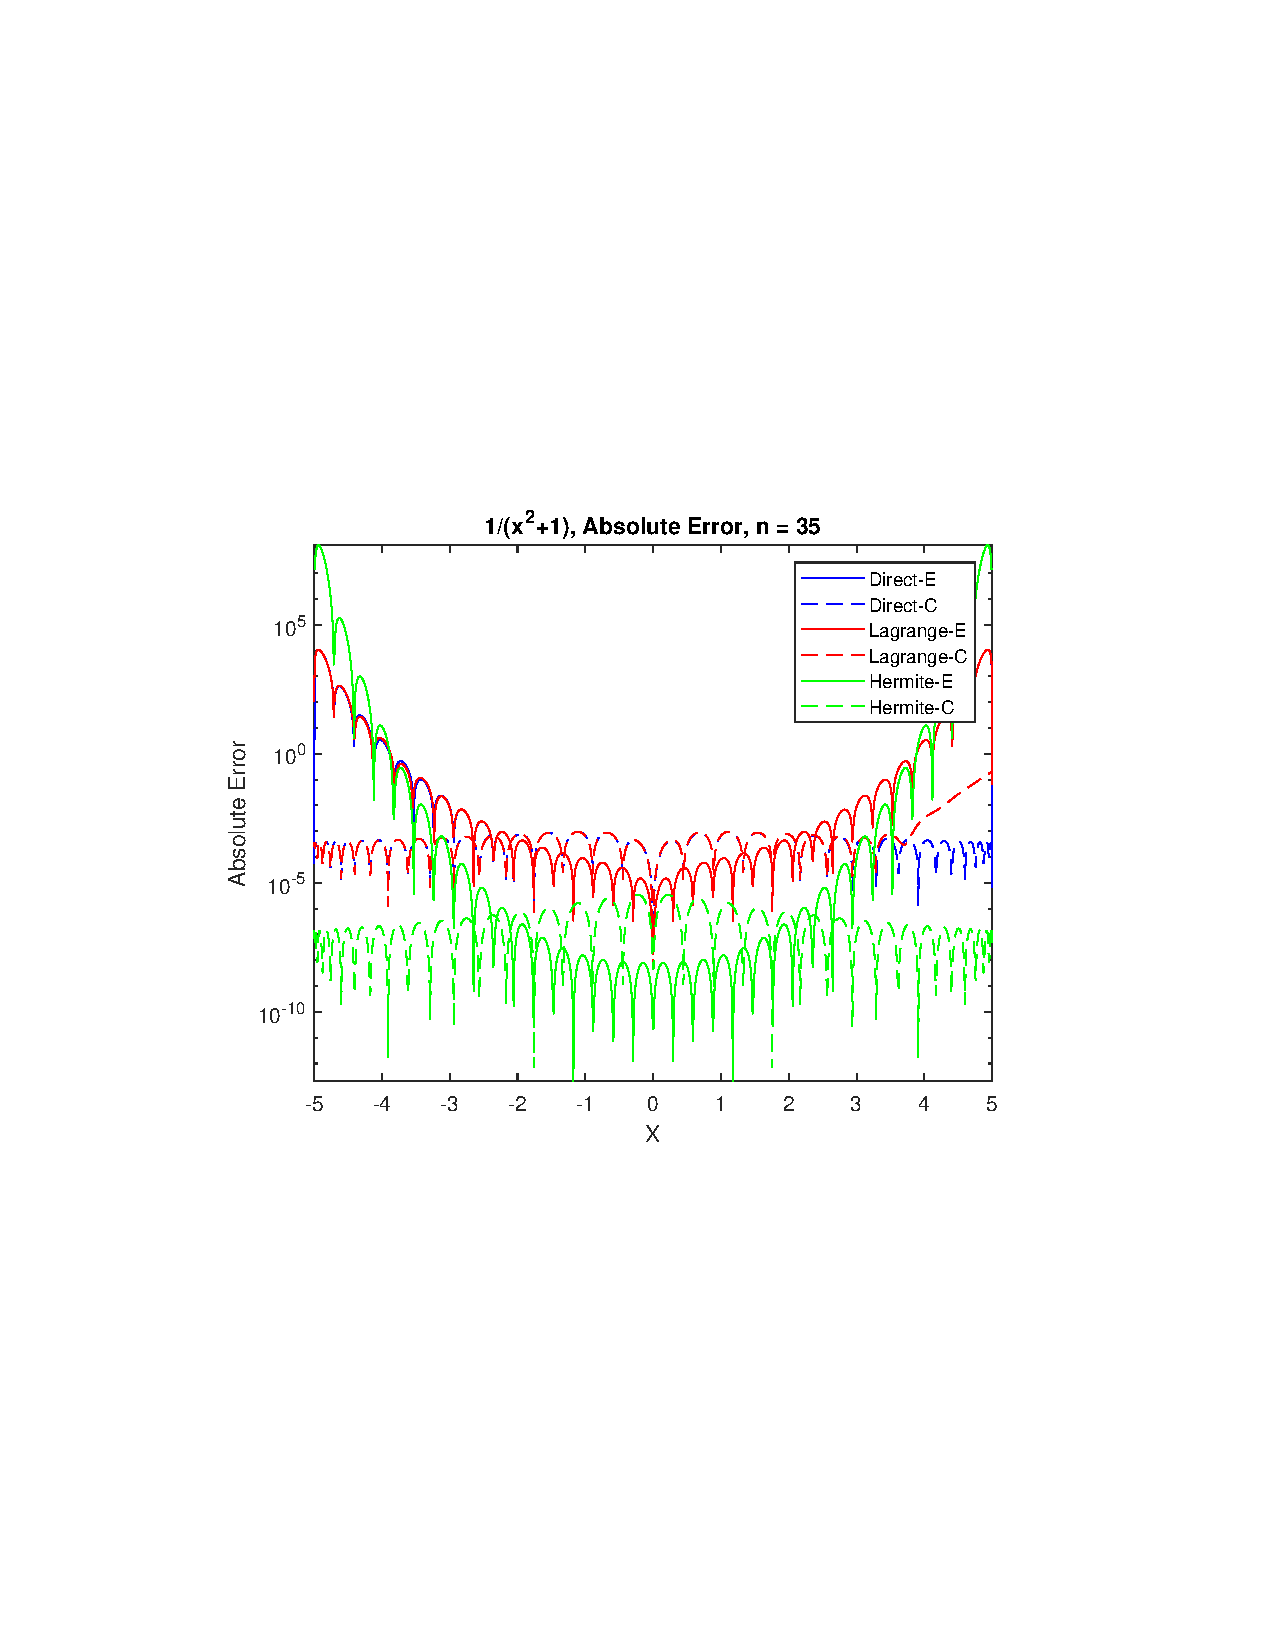
\includegraphics[width=8cm]{function3_absoluteError_35}\\

\vspace{-100pt} % I can control the vertical spacing this way.
\caption{Approximation \& error analysis of $\dfrac{1}{1+x^2}$.}
\end{figure}
%

\clearpage
\newpage
% Max Error
\subsection{Maximum Error}
\vspace{20pt} % I can control the vertical spacing this way.

\begin{figure}[h]
\centering
\vspace{-115pt} % I can control the vertical spacing this way.
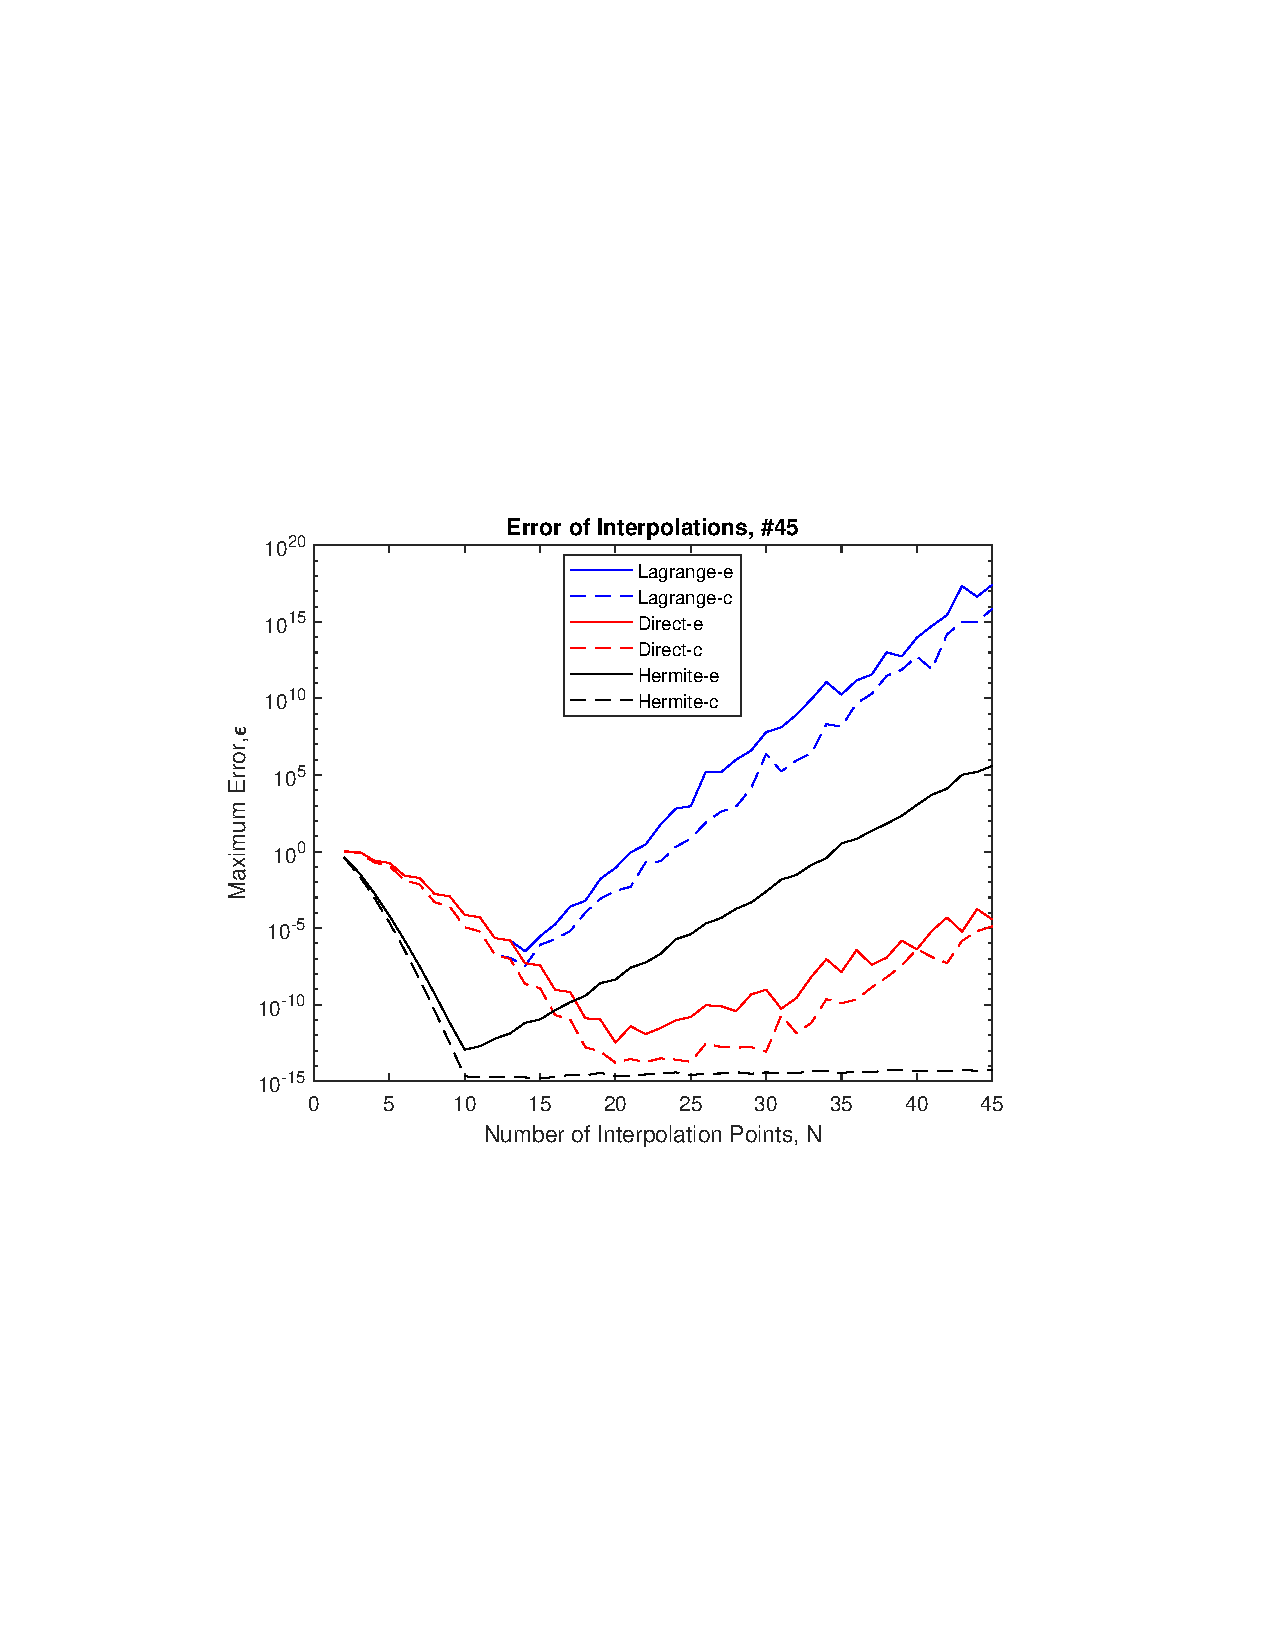
\includegraphics[width=9cm]{maxError1_45}%
\vspace{-110pt} % I can control the vertical spacing this way.
\caption{Maximum error of $Sin(x)$.}
\vspace{-80pt} % I can control the vertical spacing this way.
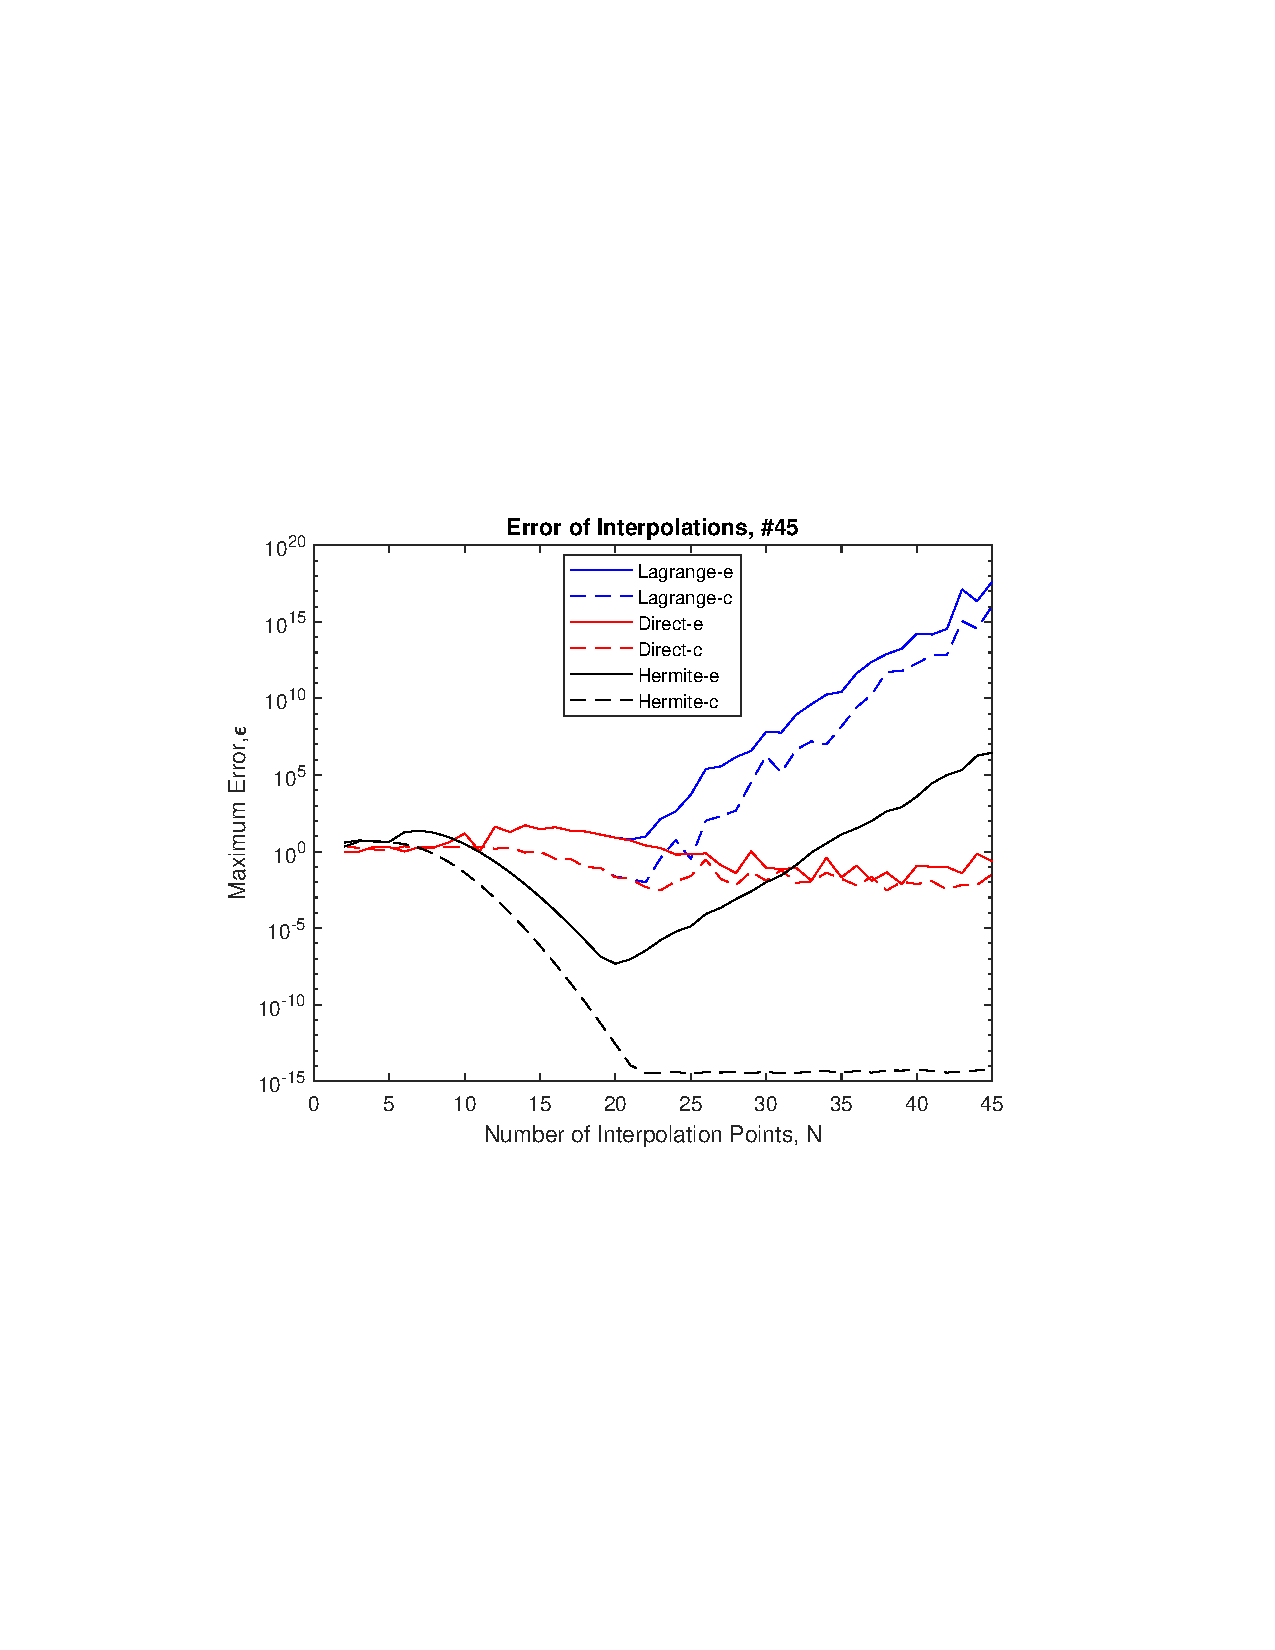
\includegraphics[width=9cm]{maxError2_45}%
\vspace{-110pt} % I can control the vertical spacing this way.
\caption{Maximum error of $Sin(5x)$.}
\vspace{-80pt} % I can control the vertical spacing this way.
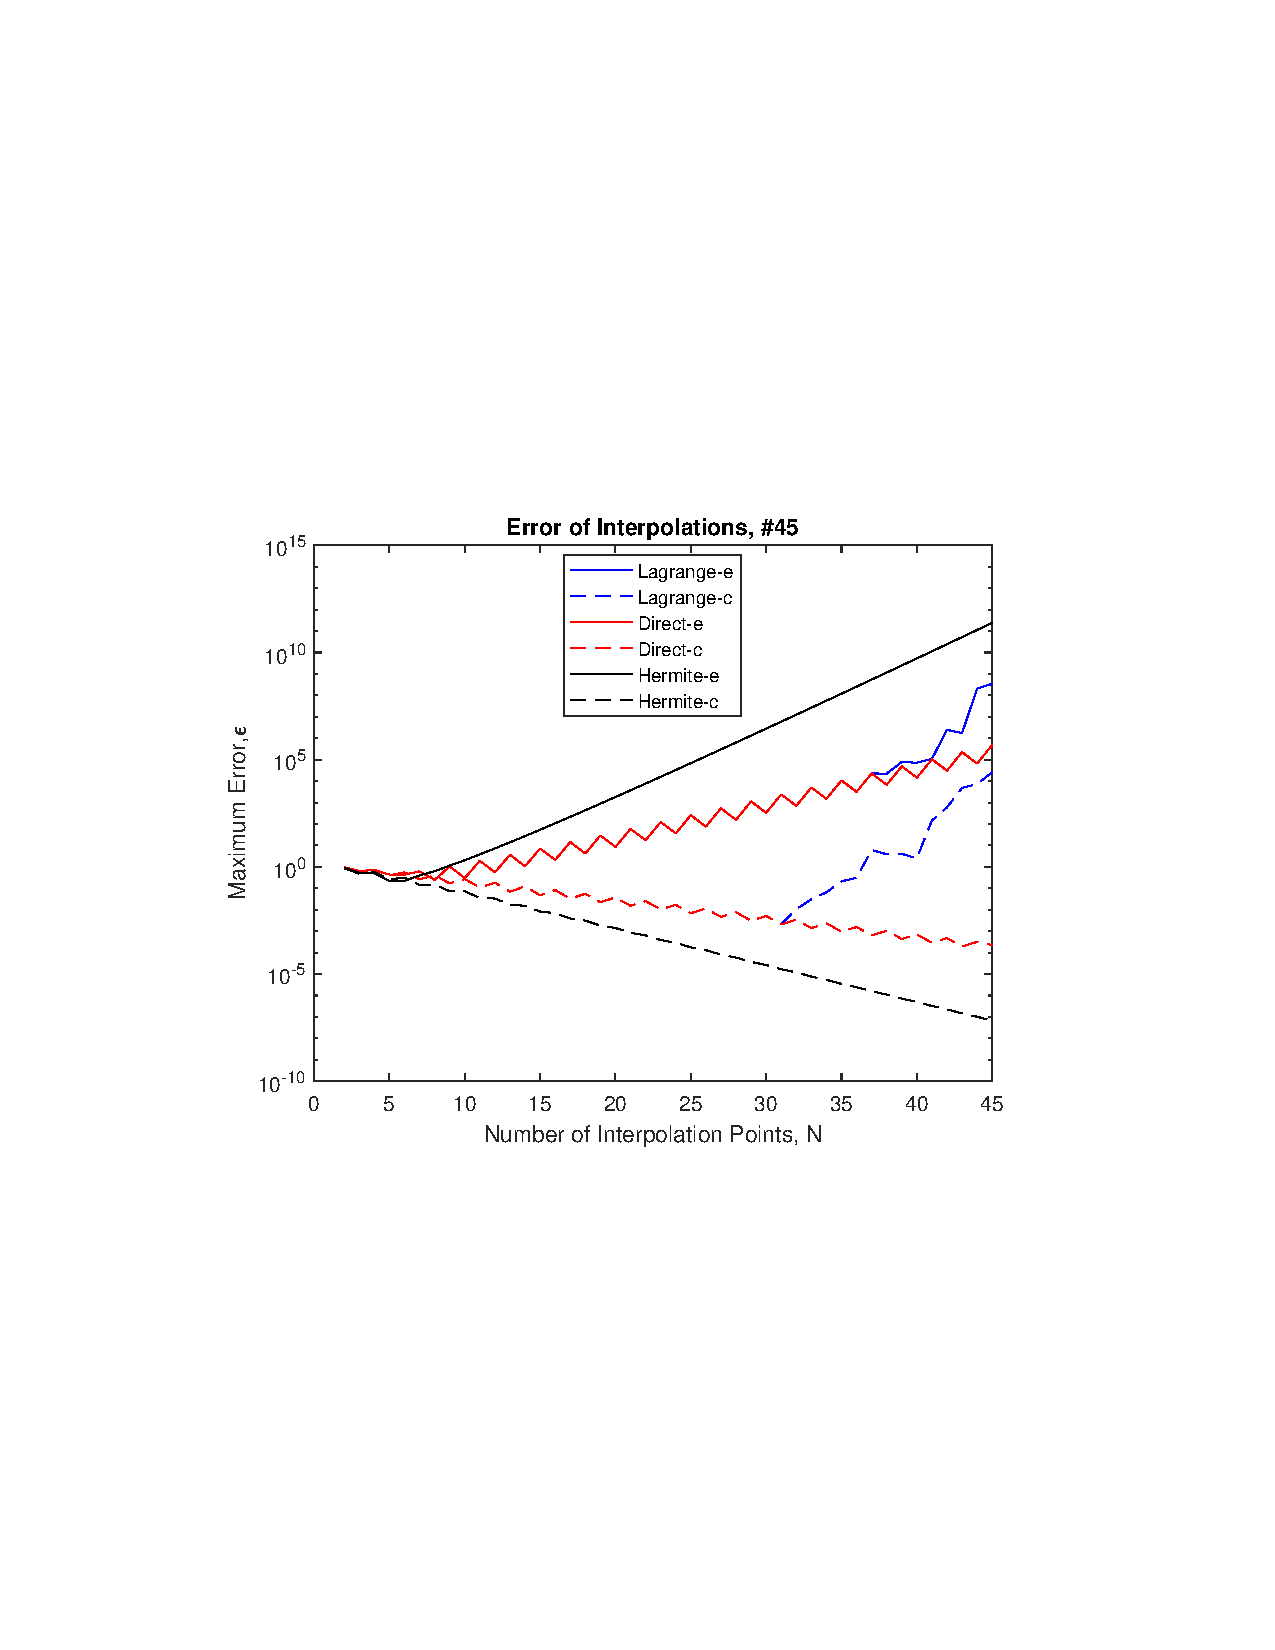
\includegraphics[width=9cm]{maxError3_45}%
\vspace{-110pt} % I can control the vertical spacing this way.
\caption{Maximum error of $\dfrac{1}{1+x^2}$.}
\end{figure}

\clearpage
\newpage
% Time
\subsection{CPU Time}

\begin{figure}[h]
\centering

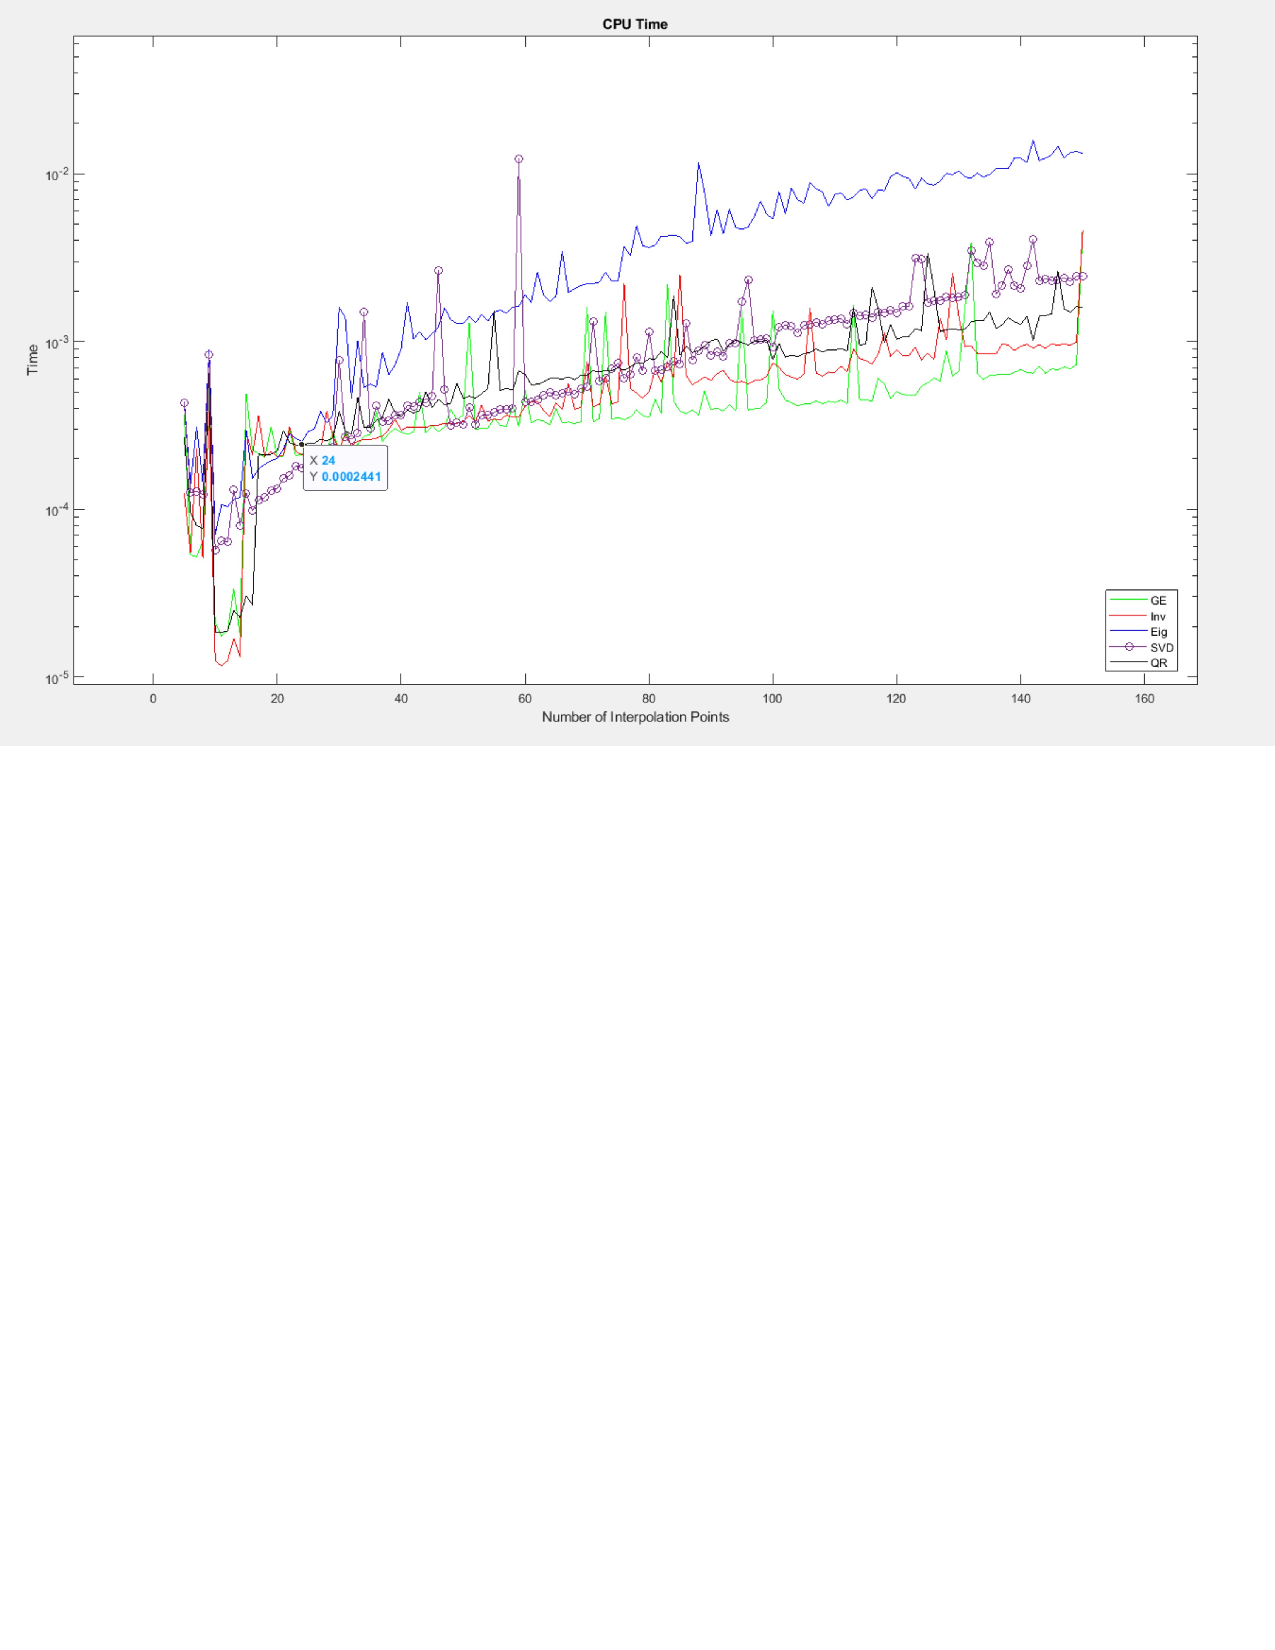
\includegraphics[width=11cm]{cpuTimes}%
\vspace{-200pt} % I can control the vertical spacing this way.
\caption{Timing various methods of solving equation \eqref{DirectEq} for the Direct method.}
\end{figure}


\clearpage
\newpage
%
\section*{Discussion}
% Paragraph 1
The error in the approximations of $Sin(x)$ for $n = 5$ can be visually seen, the curves deviate from each other by at most $10^{-1}$. The Hermite polynomials produce the lowest error with a max absolute error of approximately $10^{-4}$. The transition from $n = 10$ to $n = 15$ indicates a dramatic decrease in absolute error. The Lagrange interpolating polynomials show the highest error at this point, followed by the direct method interpolating polynomials, and finally the Hermite polynomials maintain the lowest error. Interestingly the Hermite polynomials appear to have reached the limit in error reduction, $10^{-16}$. This phenomena is due to the 16 place decimal precision of floating point numbers in MATLAB. Another interesting phenomena that can be observed is that the error curves generated by the $n$ equally spaced points begin forming a "U" shape, that is, the absolute error is much higher on the end points relative to the center of the curve. The curves generated by the Chebyshev nodes appear to be immune to this phenomenon. From $n = 25$ to $n = 35$ the error behavior for various interpolation methods is quite different. The Lagrange error (for both the Chebyshev nodes and $n$ equally spaced points) blows up and our sinusoidal wave is no longer visually perceptible in the interpolation graphs. The error of the direct method interpolating polynomials reaches an all time low at $n = 25$. At $n = 35$, the error toward the right end point, $2\pi$, starts to creep back up. By extrapolation, for progressively larger $n$ values I predict that this error will continue to get higher. The parabolic "U shape" becomes incredibly prominent for the Hermite polynomial constructed from $n$ equally spaced points. For the Hermite polynomial constructed from Chebyshev nodes the error appears to have remained constant at the lowest value from $n=15$ to $n = 35$.

% Paragraph 2
$Sin(5x)$ represents a sinusoidal wave with a higher frequency and shorter period relative to $Sin(x)$. At $n = 5$ the approximations are notably worse. Interestingly, the Lagrange polynomial from $n$ equally spaced points depicts the same approximation as it did for $Sin(x)$. This implies that we need more data points or a better heuristic for choosing data points. The Hermite polynomials also depict a lot of error. For the Hermite polynomial from $n$ equally spaced points the curve looks like a sine wave where each of the subsequent peak/ trough pairs is lowered by some linearly decreasing offset. For $n = 5$, none of the approximations are without a substantial amount of visual error and thus it is clear that more data points are needed. From $n= 10$ to $n = 15$ the Lagrange polynomials and direct method polynomials share nearly the same amount of error. This error is still suboptimal, especially at the endpoints, which depict 2 large peaks for the polynomials created from $n$ equally spaced points. The higher degree of the polynomial appears to be amplifying the end point error. The polynomials created from the Chebyshev nodes enjoy a much lower absolute error near the endpoints; however, they express a very small increase in error relative to the polynomials created from $n$ equally spaced points toward the center of the curves. From $n = 25$ to $n = 35$ a lot of interesting stuff happens. The Lagrange Chebyshev error reaches an all time low at $n = 25$, then it blows up out of control at $n = 35$. The error for the Lagrange interpolating polynomial from $n$ equally spaced points is so large at the endpoints that the peak at the endpoints becomes the only discernible feature on the interpolating polynomial graphs. The direct method polynomial error gets substantially lower and reaches an all time low at $n=35$. The Direct Chebyshev error looks better (lower) at the left end point; however, toward the center of the graph the Direct method polynomial from $n$ equally spaced points produces a lower error. The Hermite polynomial from $n$ equally spaced points expresses an all time minimum error toward the center of the curve; however, the end point error is starting to get very prominent. The Hermite from Chebyshev nodes continues to be the best approximation with the lowest overall error.

% Paragraph 3
$\dfrac{1}{1 + x^2}$ represents the first non sine function; although, visually it does look similar to $Sin(5x)$ on the interval $[1, 2.15]$. The most striking feature from these curves is how the Hermite polynomials constructed from $n$ equally spaced points absolute error at the end points blows up out of control. By $n = 35$ the error at the endpoints is $10^{7}$ and the spikes at the end points are the only discernible features on the interpolating polynomials graph. The Lagrange and Direct absolute error for $n$ equally spaced points are also bad, and actually worse than the Hermite polynomial towards the center of the curves; however, the error is nowhere near as bad at the end points. The Hermite Chebyshev polynomial produces the lowest overall absolute error again; however, it only reaches about $10^{-10}$ this time. The absolute error for the Direct Chebyshev and Lagrange Chebyshev polynomials appears to be getting incrementally better and reaches an all time low at $n = 35$ of about $10^{-5}$.

% Conclusion
\section*{Conclusion}
The clear winner in terms of minimization of the absolute error was the Hermite polynomial constructed from the Chebyshev nodes. The only cases where the absolute error was not significantly lower than the other interpolating polynomials was for small values of $n$. Another interesting observation that can be made from this experiment is that although the Chebyshev node polynomials enjoy significantly less end point error, the $n$ equally spaced points polynomials express slightly lower error towards the center of the curves. This begs the question of whether some piecewise combination of the 2 functions should be used in order to enjoy the absolute lowest overall error. In other words if you are near the end points, use the Chebyshev nodes; otherwise, use the $n$ equally spaced point polynomial. The spikes in end point error and the parabolic "U" shape observed in the error graphs is known as Runge's phenomenon, which was discussed in the background section.  Runge's phenomenon shows that higher degree polynomials do not always improve the overall accuracy of polynomial interpolation.  The difference in the error plots for $n = 5$, $Sin(x)$ and $Sin(5x)$ was interesting.  With 5 nodes, no interpolation succeeded in reducing visually perceptible error for Sin(5x); whereas, the Sin(x) interpolation yielded significantly less error.  This shows that the interpolation accuracy may be sensitive to small changes to the function being approximated.  The plot of the cpu times of the algorithms used to solve the linear system for the Direct method indicates that Eigenvalue Decomposition is approximately 1 - 2 orders of magnitude slower than the the fastest method, Guassian Elimination.  The maximum error plots show that for the $Sin(x)$ and $Sin(5x)$ the lagrange polynomials produce the most error.  For $\dfrac{1}{1+x^2}$, the Hermite polynomial constructed from $n$ equally spaced points generates tremendous error and even does worse than the Lagrange polynomials.  The Hermite-Chebyshev polynomial consistetly produces the lowest maximum error.   Further experimentation could be done with a numeric data type with more precision than MATLAB's $double$ data type. Furthermore, I could try different $n$ values, functions to approximate, methods of polynomial interpolation, and building the piecewise polynomials I described above.

% Bibliography
\begin{thebibliography}{9}

\bibitem{LHK3} Dr. Lei Hsin Kuo , ``Lecture 3 - Interpolation \& Polynomial Approximation," \emph{The University of West Florida Department of Mathematics and Statistics}, pp. 10-25, June 2021.

\bibitem{LHK4} Dr. Lei Hsin Kuo , ``Lecture 4 - Least Square Approximation \& Hermite Interpolation," \emph{The University of West Florida Department of Mathematics and Statistics}, pp. 01-25, July 2021.

\bibitem{LHK5} Dr. Lei Hsin Kuo , ``Lecture 5 - Best Approximation in Infinity Norm \& Chebyshev Polynomials," \emph{The University of West Florida Department of Mathematics and Statistics}, pp. 24-39, June 2021.

\bibitem{BJTL} Berrut, J. and Trefethen, L., 2004. Barycentric Lagrange Interpolation. SIAM Review, 46(3), pp.501-517.

\bibitem{SGW} Stewart, Gilbert W. (1996), Afternotes on Numerical Analysis, SIAM, ISBN 978-0-89871-362-6

\end{thebibliography}


\end{document}

